%% Generated by Sphinx.
\def\sphinxdocclass{report}
\documentclass[letterpaper,10pt,english]{sphinxmanual}
\ifdefined\pdfpxdimen
   \let\sphinxpxdimen\pdfpxdimen\else\newdimen\sphinxpxdimen
\fi \sphinxpxdimen=.75bp\relax

\usepackage[utf8]{inputenc}
\ifdefined\DeclareUnicodeCharacter
 \ifdefined\DeclareUnicodeCharacterAsOptional
  \DeclareUnicodeCharacter{"00A0}{\nobreakspace}
  \DeclareUnicodeCharacter{"2500}{\sphinxunichar{2500}}
  \DeclareUnicodeCharacter{"2502}{\sphinxunichar{2502}}
  \DeclareUnicodeCharacter{"2514}{\sphinxunichar{2514}}
  \DeclareUnicodeCharacter{"251C}{\sphinxunichar{251C}}
  \DeclareUnicodeCharacter{"2572}{\textbackslash}
 \else
  \DeclareUnicodeCharacter{00A0}{\nobreakspace}
  \DeclareUnicodeCharacter{2500}{\sphinxunichar{2500}}
  \DeclareUnicodeCharacter{2502}{\sphinxunichar{2502}}
  \DeclareUnicodeCharacter{2514}{\sphinxunichar{2514}}
  \DeclareUnicodeCharacter{251C}{\sphinxunichar{251C}}
  \DeclareUnicodeCharacter{2572}{\textbackslash}
 \fi
\fi
\usepackage{cmap}
\usepackage[T1]{fontenc}
\usepackage{amsmath,amssymb,amstext}
\usepackage{babel}
\usepackage{times}
\usepackage[Bjarne]{fncychap}
\usepackage[dontkeepoldnames]{sphinx}

\usepackage{geometry}

% Include hyperref last.
\usepackage{hyperref}
% Fix anchor placement for figures with captions.
\usepackage{hypcap}% it must be loaded after hyperref.
% Set up styles of URL: it should be placed after hyperref.
\urlstyle{same}
\addto\captionsenglish{\renewcommand{\contentsname}{Table of Contents}}

\addto\captionsenglish{\renewcommand{\figurename}{Fig.}}
\addto\captionsenglish{\renewcommand{\tablename}{Table}}
\addto\captionsenglish{\renewcommand{\literalblockname}{Listing}}

\addto\captionsenglish{\renewcommand{\literalblockcontinuedname}{continued from previous page}}
\addto\captionsenglish{\renewcommand{\literalblockcontinuesname}{continues on next page}}

\addto\extrasenglish{\def\pageautorefname{page}}





\title{DYCI2 library documentation}
\date{Oct 17, 2017}
\release{0.1}
\author{Jérôme Nika, IRCAM STMS LAB}
\newcommand{\sphinxlogo}{\vbox{}}
\renewcommand{\releasename}{Release}
\makeindex

\begin{document}

\maketitle
\sphinxtableofcontents
\phantomsection\label{\detokenize{index::doc}}



\chapter{\sphinxstylestrong{Introduction}}
\label{\detokenize{index:introduction}}\label{\detokenize{index:dyci2-s-documentation}}
This version of the \sphinxstyleemphasis{DYCI2 library} is the first release of a work in progress: a set of models and tools for creative generation of sequences (and in particular musical sequences) from models of sequences. It implements several models, generative heuristics, time management strategies, and architectures of interactive agents.

DYCI2 (“Creative Dynamics of Improvised Interaction”) is a collaborative research and development project funded by the French National Research Agency (ANR). It explores the creative dynamics of improvised interactions between human and artificial agents, featuring an informed artificial listening scheme, a musical structure discovery and learning scheme, and a generalized interaction / knowledge / decision dynamics scheme (see \sphinxurl{http://repmus.ircam.fr/dyci2/home}). The \sphinxstyleemphasis{DYCI2 library} is part of the DYCI2 project, it is conceived as an autonomous and easily extensible Python library, and can also be used in association with audio or midi listeners and renderers to form \sphinxstyleemphasis{DYCI2 agents} (see directory \sphinxstyleemphasis{“MaxPatches”}).

More information on the project: refer to \sphinxstylestrong{Nika, Déguernel, Chemla\textendash{}Romeu-Santos, Vincent, Assayag, “DYCI2 agents: merging the “free”, “reactive”, and “scenario-based” music generation paradigms”, in Proceedings of International Computer Music Conference 2017} (\sphinxurl{https://hal.archives-ouvertes.fr/hal-01583089/document}) (please mention this paper to mention the library).

To use the library: see the tuturials in the root directory.
\begin{description}
\item[{In this version:}] \leavevmode\begin{itemize}
\item {} 
Definitive architecture of the library: classes Model, Navigator, MetaModelNavigator, Query, Generator, GenerationHandler, and OSCAgent.

\item {} 
\sphinxstyleemphasis{Models}: Naive sequence navigation, Factor Oracle automaton.

\item {} 
\sphinxstyleemphasis{Associated navigation strategies}: free generation (“Omax-like”), single target generation, scenario-based generation (“ImproteK-like”).

\item {} 
\sphinxstyleemphasis{Architectures of generative agent}: Generator and GenerationHandler (see doc), demand-driven generative agents processing queries expressed in “events”. The (short-term and long-term) queries communicate through a shared execution trace to maintain consistency of the generated sequence when rewriting previously generated anticipations.

\item {} 
\sphinxstyleemphasis{Communication}: OSC agents embedding the generative agents.

\item {} 
\sphinxstyleemphasis{Alphabets}: Generic list labels, Chord Labels.

\item {} 
\sphinxstyleemphasis{Documentation}: modules Model, Navigator, PrefixIndexing, MetaModelNavigator, Generator, GeneratorBuilder.

\item {} 
\sphinxstyleemphasis{Tutorials}: FactorOracle, PrefixIndexing, Intervals, MetaModelNavigator, FactorOracleNavigator, Generator, GenerationHandler, OSCAgent\_Tutorial\_1 (text).

\end{itemize}

\item[{Next steps:}] \leavevmode\begin{itemize}
\item {} 
\sphinxstyleemphasis{Models}: N-gram.

\item {} 
\sphinxstyleemphasis{Associated navigation strategies}: Navigator including a notion of “activity profile”, free generation and single target generation using this navigator  (“Somax-like”).

\item {} 
\sphinxstyleemphasis{Architectures of generative agent}: “Algebra” of queries, queries expressed in “ms”. output of the queries not directly outputted but redirected to a choice method that will be in charge of outputting the result \textendash{}\textgreater{} new playing modes “hard hybrid guidance” (long-term queries \textgreater{} short-term queries) and “soft hybrid guidance” (short-term queries \textgreater{} long-term queries).

\item {} 
\sphinxstyleemphasis{Alphabets}: Class “contents”.

\item {} 
\sphinxstyleemphasis{Documentation}: modules Label, Transforms, Intervals, ParseAnnotationFiles, CorpusBuilder, OSCAgent.

\item {} 
\sphinxstyleemphasis{Tutorials}: GeneratorBuilder, OSCAgent\_Tutorial\_2 (audio), OSCAgent\_Tutorial\_3 (midi).

\end{itemize}

\end{description}


\chapter{\sphinxstylestrong{Overview}}
\label{\detokenize{index:overview}}
\begin{figure}[htbp]
\centering
\capstart

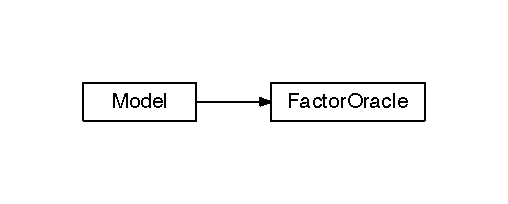
\includegraphics{inheritance-425337933f1f8a96ede832a451dc0704d5ae3c99.pdf}
\caption{{\hyperref[\detokenize{index:Model.Model}]{\sphinxcrossref{\sphinxcode{Model}}}} is an abstract class. Any new model of sequence must inherit from this class. The classes inheriting from this class are minimal and only implement the construction algorithms and basic methods. Navigation and creative aspects are handled by the classes introduced below. Models of sequence implemented so far: Factor Oracle Automaton ({\hyperref[\detokenize{index:Model.FactorOracle}]{\sphinxcrossref{\sphinxcode{FactorOracle}}}}).}\label{\detokenize{index:id1}}\end{figure}

\begin{figure}[htbp]
\centering
\capstart

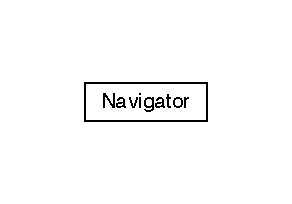
\includegraphics{inheritance-111a3bc16fdc4ecb7d225978d938cca5aadd22cc.pdf}
\caption{The class {\hyperref[\detokenize{index:Navigator.Navigator}]{\sphinxcrossref{\sphinxcode{Navigator}}}} implements parameters and methods that are used to navigate through a model of sequence. These parameters and methods are \sphinxstylestrong{model-independent}. This class defines in particular the naive versions of the methods {\hyperref[\detokenize{index:Navigator.Navigator.simply_guided_generation}]{\sphinxcrossref{\sphinxcode{simply\_guided\_generation()}}}} and {\hyperref[\detokenize{index:Navigator.Navigator.free_generation}]{\sphinxcrossref{\sphinxcode{free\_generation()}}}} handling the navigation through a sequence when it is respectively guided by target labels and free. These methods are overloaded by model-dependant versions (and other model-dependent parameters or methods can be added) when creating a \sphinxstylestrong{model navigator} class (cf. below).}\label{\detokenize{index:id2}}\end{figure}

\begin{figure}[htbp]
\centering
\capstart

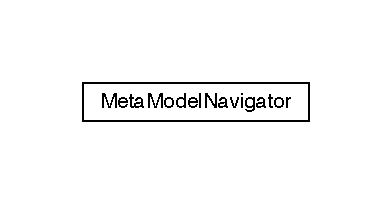
\includegraphics{inheritance-14f94ff1ec9591fb712946f283f0fea99a890a19.pdf}
\caption{{\hyperref[\detokenize{index:MetaModelNavigator.MetaModelNavigator}]{\sphinxcrossref{\sphinxcode{MetaModelNavigator}}}} is a \sphinxstylestrong{metaclass}. A new class created using this metaclass is a \sphinxstylestrong{model navigator} and inherits from: \sphinxstylestrong{1)} a class inheriting from {\hyperref[\detokenize{index:Model.Model}]{\sphinxcrossref{\sphinxcode{Model}}}}, \sphinxstylestrong{2)} a class inheriting from {\hyperref[\detokenize{index:Navigator.Navigator}]{\sphinxcrossref{\sphinxcode{Navigator}}}}. A \sphinxstylestrong{model navigator} implements the different algorithms, strategies, and heuristics to navigate through a given model of sequence for analysis or creative applications, for example \sphinxstylestrong{generating new sequences using concatenative synthesis of events learned in the model}. The class {\hyperref[\detokenize{index:ModelNavigator.FactorOracleNavigator}]{\sphinxcrossref{\sphinxcode{FactorOracleNavigator}}}} introduced below is an example of model navigator created using this metaclass.}\label{\detokenize{index:id3}}\end{figure}

\begin{figure}[htbp]
\centering
\capstart

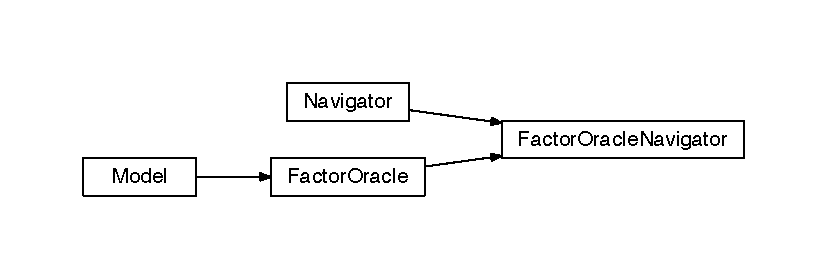
\includegraphics{inheritance-8880bdc449e3d4349093afc4177dfb2922cdb418.pdf}
\caption{The class {\hyperref[\detokenize{index:ModelNavigator.FactorOracleNavigator}]{\sphinxcrossref{\sphinxcode{FactorOracleNavigator}}}} implements different algorithms, strategies, and heuristics to navigate through a Factor Oracle Automaton for creative applications. The creation of the class {\hyperref[\detokenize{index:ModelNavigator.FactorOracleNavigator}]{\sphinxcrossref{\sphinxcode{FactorOracleNavigator}}}} in the file \sphinxcode{ModelNavigator.py} gives an example of easy definition of a new class of model navigator using the metaclass {\hyperref[\detokenize{index:MetaModelNavigator.MetaModelNavigator}]{\sphinxcrossref{\sphinxcode{MetaModelNavigator}}}}: 1) chose two bases (here, model = {\hyperref[\detokenize{index:Model.FactorOracle}]{\sphinxcrossref{\sphinxcode{FactorOracle}}}}, navigator = {\hyperref[\detokenize{index:Navigator.Navigator}]{\sphinxcrossref{\sphinxcode{Navigator}}}}), 2) define the methods to overload {\hyperref[\detokenize{index:Navigator.Navigator.simply_guided_generation}]{\sphinxcrossref{\sphinxcode{simply\_guided\_generation()}}}} and {\hyperref[\detokenize{index:Navigator.Navigator.free_generation}]{\sphinxcrossref{\sphinxcode{free\_generation()}}}} (here {\hyperref[\detokenize{index:ModelNavigator.FactorOracleNavigator.simply_guided_navigation}]{\sphinxcrossref{\sphinxcode{ModelNavigator.FactorOracleNavigator.simply\_guided\_navigation()}}}} and {\hyperref[\detokenize{index:ModelNavigator.FactorOracleNavigator.free_navigation}]{\sphinxcrossref{\sphinxcode{ModelNavigator.FactorOracleNavigator.free\_navigation()}}}})}\label{\detokenize{index:id4}}\end{figure}

\begin{figure}[htbp]
\centering
\capstart

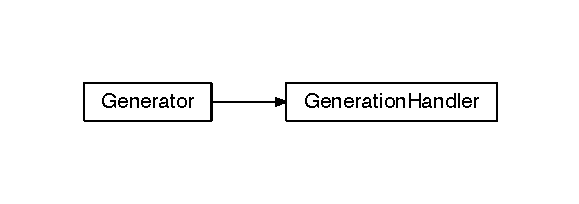
\includegraphics{inheritance-45389eff6d71c56e9ebdb1c18f0709c68c075428.pdf}
\caption{The class {\hyperref[\detokenize{index:Generator.Generator}]{\sphinxcrossref{\sphinxcode{Generator}}}} embeds a \sphinxstylestrong{model navigator} (cf. metaclass {\hyperref[\detokenize{index:MetaModelNavigator.MetaModelNavigator}]{\sphinxcrossref{\sphinxcode{MetaModelNavigator}}}}) as “memory” and processes \sphinxstylestrong{queries} (class {\hyperref[\detokenize{index:Query.Query}]{\sphinxcrossref{\sphinxcode{Query}}}}) to generate new sequences. This class uses pattern matching techniques (cf. {\hyperref[\detokenize{index:module-PrefixIndexing}]{\sphinxcrossref{\sphinxcode{PrefixIndexing}}}}) to enrich the navigation and generation methods offered by the chosen model. The class {\hyperref[\detokenize{index:Generator.GenerationHandler}]{\sphinxcrossref{\sphinxcode{GenerationHandler}}}} introduces time management and planning for interactive applications and adds a pool of query, concurrency (e.g. processing of concurrent queries), etc. to the class {\hyperref[\detokenize{index:Generator.Generator}]{\sphinxcrossref{\sphinxcode{Generator}}}}.}\label{\detokenize{index:id5}}\end{figure}

\begin{figure}[htbp]
\centering
\capstart

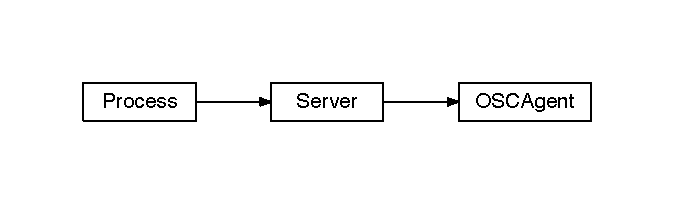
\includegraphics{inheritance-def9fd93a357ceca4452c5c313a453f38e18390c.pdf}
\caption{The class \sphinxcode{Server} defines an OSC (\sphinxurl{http://opensoundcontrol.org}) server to communicate with external applications. The class \sphinxcode{OSCAgent} defines a process embedding an instance of {\hyperref[\detokenize{index:Generator.GenerationHandler}]{\sphinxcrossref{\sphinxcode{GenerationHandler}}}} and its own OSC sender, receiver, settings, etc. to receive queries and control parameters and send generation outputs. Both classes can be used in particular in association with a Max interface handling audio or midi rendering.}\label{\detokenize{index:id6}}\end{figure}


\chapter{\sphinxstylestrong{Models and navigation}}
\label{\detokenize{index:module-Model}}\label{\detokenize{index:models-and-navigation}}\index{Model (module)}

\section{Model}
\label{\detokenize{index:model}}
This module defines different models of symbolic sequences.
The classes defined in this module are minimal and only implement the construction algorithms and basic methods. Navigation and creative aspects are handled by other classes in the library (cf. {\hyperref[\detokenize{index:module-Navigator}]{\sphinxcrossref{\sphinxcode{Navigator}}}} and \sphinxcode{ModelNavigator}).
Main classes: {\hyperref[\detokenize{index:Model.Model}]{\sphinxcrossref{\sphinxcode{Model}}}}, {\hyperref[\detokenize{index:Model.FactorOracle}]{\sphinxcrossref{\sphinxcode{FactorOracle}}}}. 
Tutorial for the class {\hyperref[\detokenize{index:Model.FactorOracle}]{\sphinxcrossref{\sphinxcode{FactorOracle}}}} in \sphinxcode{\_Tutorials\_/FactorOracleAutomaton\_tutorial.py}.
\index{FactorOracle (class in Model)}

\begin{fulllineitems}
\phantomsection\label{\detokenize{index:Model.FactorOracle}}\pysiglinewithargsret{\sphinxbfcode{class }\sphinxcode{Model.}\sphinxbfcode{FactorOracle}}{\emph{sequence={[}{]}}, \emph{labels={[}{]}}, \emph{equiv=\textless{}function \textless{}lambda\textgreater{}\textgreater{}}}{}
Bases: {\hyperref[\detokenize{index:Model.Model}]{\sphinxcrossref{\sphinxcode{Model.Model}}}}

\sphinxstylestrong{Factor Oracle automaton class.}
Implementation of the Factor Oracle Automaton (Allauzen, Crochemore, Raffinot, 1999).
Convention: since the all the transitions arriving in a same state have the same label, 
the labels are not carried by the transitions but by the states.
\begin{quote}\begin{description}
\item[{Parameters}] \leavevmode\begin{itemize}
\item {} 
\sphinxstyleliteralstrong{sequence} (\sphinxstyleliteralemphasis{list}\sphinxstyleliteralemphasis{ or }\sphinxhref{https://docs.python.org/2/library/functions.html\#str}{\sphinxstyleliteralemphasis{str}}) \textendash{} sequence learnt in the Factor Oracle automaton

\item {} 
\sphinxstyleliteralstrong{labels} (\sphinxstyleliteralemphasis{list}\sphinxstyleliteralemphasis{ or }\sphinxhref{https://docs.python.org/2/library/functions.html\#str}{\sphinxstyleliteralemphasis{str}}) \textendash{} sequence of labels chosen to describe the sequence

\item {} 
\sphinxstyleliteralstrong{direct\_transitions} (\sphinxhref{https://docs.python.org/2/library/stdtypes.html\#dict}{\sphinxstyleliteralemphasis{dict}}) \textendash{} direct transitions in the automaton (key = index state 1, value = tuple: label, index state 2)

\item {} 
\sphinxstyleliteralstrong{factor\_links} (\sphinxhref{https://docs.python.org/2/library/stdtypes.html\#dict}{\sphinxstyleliteralemphasis{dict}}) \textendash{} factor links in the automaton (key = index state 1, value = list of tuples: (label, index state 2)

\item {} 
\sphinxstyleliteralstrong{suffix\_links} (\sphinxhref{https://docs.python.org/2/library/stdtypes.html\#dict}{\sphinxstyleliteralemphasis{dict}}) \textendash{} suffix links in the automaton (key = index state 1, value = index state 2)

\item {} 
\sphinxstyleliteralstrong{reverse\_suffix\_links} (\sphinxhref{https://docs.python.org/2/library/stdtypes.html\#dict}{\sphinxstyleliteralemphasis{dict}}) \textendash{} reverse suffix links in the automaton (key = index state 1, value = list of index state 2)

\item {} 
\sphinxstyleliteralstrong{equiv} (\sphinxstyleliteralemphasis{function}) \textendash{} compararison function given as a lambda function, default: (lambda x,y : x == y).

\end{itemize}

\item[{!}] \leavevmode
\sphinxstylestrong{equiv} has to be consistent with the type of the elements in labels.

\item[{See also}] \leavevmode
\sphinxstylestrong{Tutorial in} \sphinxcode{\_Tutorials\_/FactorOracleAutomaton\_tutorial.py}.

\end{description}\end{quote}

(When there is no need to distinguish the sequence and its labels : FactorOracle(sequence,sequence).)
\begin{quote}\begin{description}
\item[{Example}] \leavevmode
\end{description}\end{quote}

\begin{sphinxVerbatim}[commandchars=\\\{\}]
\PYG{g+gp}{\PYGZgt{}\PYGZgt{}\PYGZgt{} }\PYG{n}{sequence} \PYG{o}{=} \PYG{p}{[}\PYG{l+s+s1}{\PYGZsq{}}\PYG{l+s+s1}{A}\PYG{l+s+s1}{\PYGZsq{}}\PYG{p}{,}\PYG{l+s+s1}{\PYGZsq{}}\PYG{l+s+s1}{B}\PYG{l+s+s1}{\PYGZsq{}}\PYG{p}{,}\PYG{l+s+s1}{\PYGZsq{}}\PYG{l+s+s1}{B}\PYG{l+s+s1}{\PYGZsq{}}\PYG{p}{,}\PYG{l+s+s1}{\PYGZsq{}}\PYG{l+s+s1}{C}\PYG{l+s+s1}{\PYGZsq{}}\PYG{p}{,}\PYG{l+s+s1}{\PYGZsq{}}\PYG{l+s+s1}{A}\PYG{l+s+s1}{\PYGZsq{}}\PYG{p}{,}\PYG{l+s+s1}{\PYGZsq{}}\PYG{l+s+s1}{B}\PYG{l+s+s1}{\PYGZsq{}}\PYG{p}{,}\PYG{l+s+s1}{\PYGZsq{}}\PYG{l+s+s1}{C}\PYG{l+s+s1}{\PYGZsq{}}\PYG{p}{,}\PYG{l+s+s1}{\PYGZsq{}}\PYG{l+s+s1}{D}\PYG{l+s+s1}{\PYGZsq{}}\PYG{p}{,}\PYG{l+s+s1}{\PYGZsq{}}\PYG{l+s+s1}{A}\PYG{l+s+s1}{\PYGZsq{}}\PYG{p}{,}\PYG{l+s+s1}{\PYGZsq{}}\PYG{l+s+s1}{B}\PYG{l+s+s1}{\PYGZsq{}}\PYG{p}{,}\PYG{l+s+s1}{\PYGZsq{}}\PYG{l+s+s1}{C}\PYG{l+s+s1}{\PYGZsq{}}\PYG{p}{]}
\PYG{g+gp}{\PYGZgt{}\PYGZgt{}\PYGZgt{} }\PYG{n}{FO} \PYG{o}{=} \PYG{n}{FactorOracle}\PYG{p}{(}\PYG{n}{sequence}\PYG{p}{,} \PYG{n}{sequence}\PYG{p}{)}
\PYG{g+gp}{\PYGZgt{}\PYGZgt{}\PYGZgt{} }
\PYG{g+gp}{\PYGZgt{}\PYGZgt{}\PYGZgt{} }\PYG{n}{sequence} \PYG{o}{=} \PYG{p}{[}\PYG{l+s+s1}{\PYGZsq{}}\PYG{l+s+s1}{A1}\PYG{l+s+s1}{\PYGZsq{}}\PYG{p}{,}\PYG{l+s+s1}{\PYGZsq{}}\PYG{l+s+s1}{B1}\PYG{l+s+s1}{\PYGZsq{}}\PYG{p}{,}\PYG{l+s+s1}{\PYGZsq{}}\PYG{l+s+s1}{B2}\PYG{l+s+s1}{\PYGZsq{}}\PYG{p}{,}\PYG{l+s+s1}{\PYGZsq{}}\PYG{l+s+s1}{C1}\PYG{l+s+s1}{\PYGZsq{}}\PYG{p}{,}\PYG{l+s+s1}{\PYGZsq{}}\PYG{l+s+s1}{A2}\PYG{l+s+s1}{\PYGZsq{}}\PYG{p}{,}\PYG{l+s+s1}{\PYGZsq{}}\PYG{l+s+s1}{B3}\PYG{l+s+s1}{\PYGZsq{}}\PYG{p}{,}\PYG{l+s+s1}{\PYGZsq{}}\PYG{l+s+s1}{C2}\PYG{l+s+s1}{\PYGZsq{}}\PYG{p}{,}\PYG{l+s+s1}{\PYGZsq{}}\PYG{l+s+s1}{D1}\PYG{l+s+s1}{\PYGZsq{}}\PYG{p}{,}\PYG{l+s+s1}{\PYGZsq{}}\PYG{l+s+s1}{A3}\PYG{l+s+s1}{\PYGZsq{}}\PYG{p}{,}\PYG{l+s+s1}{\PYGZsq{}}\PYG{l+s+s1}{B4}\PYG{l+s+s1}{\PYGZsq{}}\PYG{p}{,}\PYG{l+s+s1}{\PYGZsq{}}\PYG{l+s+s1}{C3}\PYG{l+s+s1}{\PYGZsq{}}\PYG{p}{]}
\PYG{g+gp}{\PYGZgt{}\PYGZgt{}\PYGZgt{} }\PYG{n}{labels} \PYG{o}{=} \PYG{p}{[}\PYG{n}{s}\PYG{p}{[}\PYG{l+m+mi}{0}\PYG{p}{]} \PYG{k}{for} \PYG{n}{s} \PYG{o+ow}{in} \PYG{n}{sequence}\PYG{p}{]}
\PYG{g+gp}{\PYGZgt{}\PYGZgt{}\PYGZgt{} }\PYG{n}{FO\PYGZus{}2} \PYG{o}{=} \PYG{n}{FactorOracle}\PYG{p}{(}\PYG{n}{sequence}\PYG{p}{,} \PYG{n}{labels}\PYG{p}{)}
\PYG{g+gp}{\PYGZgt{}\PYGZgt{}\PYGZgt{} }
\PYG{g+gp}{\PYGZgt{}\PYGZgt{}\PYGZgt{} }\PYG{n}{equiv\PYGZus{}AC\PYGZus{}BD} \PYG{o}{=} \PYG{p}{(}\PYG{k}{lambda} \PYG{n}{x}\PYG{p}{,}\PYG{n}{y}\PYG{p}{:} \PYG{n+nb}{set}\PYG{p}{(}\PYG{p}{[}\PYG{n}{x}\PYG{p}{,}\PYG{n}{y}\PYG{p}{]}\PYG{p}{)}\PYG{o}{.}\PYG{n}{issubset}\PYG{p}{(}\PYG{n+nb}{set}\PYG{p}{(}\PYG{p}{[}\PYG{l+s+s1}{\PYGZsq{}}\PYG{l+s+s1}{A}\PYG{l+s+s1}{\PYGZsq{}}\PYG{p}{,}\PYG{l+s+s1}{\PYGZsq{}}\PYG{l+s+s1}{C}\PYG{l+s+s1}{\PYGZsq{}}\PYG{p}{]}\PYG{p}{)}\PYG{p}{)} \PYG{o+ow}{or} \PYG{n+nb}{set}\PYG{p}{(}\PYG{p}{[}\PYG{n}{x}\PYG{p}{,}\PYG{n}{y}\PYG{p}{]}\PYG{p}{)}\PYG{o}{.}\PYG{n}{issubset}\PYG{p}{(}\PYG{n+nb}{set}\PYG{p}{(}\PYG{p}{[}\PYG{l+s+s1}{\PYGZsq{}}\PYG{l+s+s1}{B}\PYG{l+s+s1}{\PYGZsq{}}\PYG{p}{,}\PYG{l+s+s1}{\PYGZsq{}}\PYG{l+s+s1}{D}\PYG{l+s+s1}{\PYGZsq{}}\PYG{p}{]}\PYG{p}{)}\PYG{p}{)}\PYG{p}{)}
\PYG{g+gp}{\PYGZgt{}\PYGZgt{}\PYGZgt{} }\PYG{n}{FO\PYGZus{}3} \PYG{o}{=} \PYG{n}{FactorOracle}\PYG{p}{(}\PYG{n}{sequence}\PYG{p}{,} \PYG{n}{labels}\PYG{p}{,} \PYG{n}{equiv\PYGZus{}AC\PYGZus{}BD}\PYG{p}{)}
\end{sphinxVerbatim}
\index{add\_direct\_transition() (Model.FactorOracle method)}

\begin{fulllineitems}
\phantomsection\label{\detokenize{index:Model.FactorOracle.add_direct_transition}}\pysiglinewithargsret{\sphinxbfcode{add\_direct\_transition}}{\emph{index\_state1}, \emph{label}, \emph{index\_state2}}{}
Adds a transition labelled by ‘label’ from the state at index ‘index\_state1’ to the state at index ‘index\_state2’ in the Factor Oracle automaton.

\end{fulllineitems}

\index{add\_factor\_link() (Model.FactorOracle method)}

\begin{fulllineitems}
\phantomsection\label{\detokenize{index:Model.FactorOracle.add_factor_link}}\pysiglinewithargsret{\sphinxbfcode{add\_factor\_link}}{\emph{index\_state1}, \emph{label}, \emph{index\_state2}}{}
Adds a factor link labelled by ‘label’ from the state at index ‘index\_state1’ to the state at index ‘index\_state2’ in the Factor Oracle automaton.

\end{fulllineitems}

\index{add\_suffix\_link() (Model.FactorOracle method)}

\begin{fulllineitems}
\phantomsection\label{\detokenize{index:Model.FactorOracle.add_suffix_link}}\pysiglinewithargsret{\sphinxbfcode{add\_suffix\_link}}{\emph{index\_state1}, \emph{index\_state2}}{}
Adds a suffix link (and the associated reverse suffix link) from the state at index ‘index\_state1’ to the state at index ‘index\_state2’ in the Factor Oracle automaton.

\end{fulllineitems}

\index{continuations() (Model.FactorOracle method)}

\begin{fulllineitems}
\phantomsection\label{\detokenize{index:Model.FactorOracle.continuations}}\pysiglinewithargsret{\sphinxbfcode{continuations}}{\emph{index\_state}, \emph{forward\_context\_length\_min=1}, \emph{equiv=None}, \emph{authorize\_direct\_transition=True}}{}
Possible continuations from the state at index index\_state in the automaton, i.e. direct transition and states reached using suffix links and reverse suffix links.
These states follow states sharing a common backward context and a common forward context with the state at index index\_state in the automaton. 
The lengths of the common backward contexts are given by the Factor Oracle automaton, the forward context is imposed by a parameter.
\begin{quote}\begin{description}
\item[{Parameters}] \leavevmode\begin{itemize}
\item {} 
\sphinxstyleliteralstrong{index\_state} (\sphinxhref{https://docs.python.org/2/library/functions.html\#int}{\sphinxstyleliteralemphasis{int}}) \textendash{} start index

\item {} 
\sphinxstyleliteralstrong{forward\_context\_length\_min} (\sphinxhref{https://docs.python.org/2/library/functions.html\#int}{\sphinxstyleliteralemphasis{int}}) \textendash{} minimum length of the forward common context

\item {} 
\sphinxstyleliteralstrong{equiv} (\sphinxstyleliteralemphasis{function}) \textendash{} Compararison function given as a lambda function, default: self.equiv.

\item {} 
\sphinxstyleliteralstrong{authorize\_direct\_transition} (\sphinxhref{https://docs.python.org/2/library/functions.html\#bool}{\sphinxstyleliteralemphasis{bool}}) \textendash{} include direct transitions ?

\end{itemize}

\item[{Returns}] \leavevmode
Indexes in the automaton of the possible continuations from the state at index index\_state in the automaton.

\item[{Return type}] \leavevmode
list (\sphinxhref{https://docs.python.org/2/library/functions.html\#int}{int})

\item[{See also}] \leavevmode
\sphinxstylestrong{Tutorial in} \sphinxcode{\_Tutorials\_/FactorOracleAutomaton\_tutorial.py}.

\item[{!}] \leavevmode
\sphinxstylestrong{equiv} has to be consistent with the type of the elements in labels.

\item[{Example}] \leavevmode
\end{description}\end{quote}

\begin{sphinxVerbatim}[commandchars=\\\{\}]
\PYG{g+gp}{\PYGZgt{}\PYGZgt{}\PYGZgt{} }\PYG{n}{sequence} \PYG{o}{=} \PYG{p}{[}\PYG{l+s+s1}{\PYGZsq{}}\PYG{l+s+s1}{A1}\PYG{l+s+s1}{\PYGZsq{}}\PYG{p}{,}\PYG{l+s+s1}{\PYGZsq{}}\PYG{l+s+s1}{B1}\PYG{l+s+s1}{\PYGZsq{}}\PYG{p}{,}\PYG{l+s+s1}{\PYGZsq{}}\PYG{l+s+s1}{B2}\PYG{l+s+s1}{\PYGZsq{}}\PYG{p}{,}\PYG{l+s+s1}{\PYGZsq{}}\PYG{l+s+s1}{C1}\PYG{l+s+s1}{\PYGZsq{}}\PYG{p}{,}\PYG{l+s+s1}{\PYGZsq{}}\PYG{l+s+s1}{A2}\PYG{l+s+s1}{\PYGZsq{}}\PYG{p}{,}\PYG{l+s+s1}{\PYGZsq{}}\PYG{l+s+s1}{B3}\PYG{l+s+s1}{\PYGZsq{}}\PYG{p}{,}\PYG{l+s+s1}{\PYGZsq{}}\PYG{l+s+s1}{C2}\PYG{l+s+s1}{\PYGZsq{}}\PYG{p}{,}\PYG{l+s+s1}{\PYGZsq{}}\PYG{l+s+s1}{D1}\PYG{l+s+s1}{\PYGZsq{}}\PYG{p}{,}\PYG{l+s+s1}{\PYGZsq{}}\PYG{l+s+s1}{A3}\PYG{l+s+s1}{\PYGZsq{}}\PYG{p}{,}\PYG{l+s+s1}{\PYGZsq{}}\PYG{l+s+s1}{B4}\PYG{l+s+s1}{\PYGZsq{}}\PYG{p}{,}\PYG{l+s+s1}{\PYGZsq{}}\PYG{l+s+s1}{C3}\PYG{l+s+s1}{\PYGZsq{}}\PYG{p}{]}
\PYG{g+gp}{\PYGZgt{}\PYGZgt{}\PYGZgt{} }\PYG{n}{labels} \PYG{o}{=} \PYG{p}{[}\PYG{n}{s}\PYG{p}{[}\PYG{l+m+mi}{0}\PYG{p}{]} \PYG{k}{for} \PYG{n}{s} \PYG{o+ow}{in} \PYG{n}{sequence}\PYG{p}{]}
\PYG{g+gp}{\PYGZgt{}\PYGZgt{}\PYGZgt{} }\PYG{n}{FON} \PYG{o}{=} \PYG{n}{FactorOracleNavigator}\PYG{p}{(}\PYG{n}{sequence}\PYG{p}{,} \PYG{n}{labels}\PYG{p}{)}
\PYG{g+gp}{\PYGZgt{}\PYGZgt{}\PYGZgt{} }
\PYG{g+gp}{\PYGZgt{}\PYGZgt{}\PYGZgt{} }\PYG{n}{index} \PYG{o}{=} \PYG{l+m+mi}{6}
\PYG{g+gp}{\PYGZgt{}\PYGZgt{}\PYGZgt{} }\PYG{n}{forward\PYGZus{}context\PYGZus{}length\PYGZus{}min} \PYG{o}{=} \PYG{l+m+mi}{1}
\PYG{g+gp}{\PYGZgt{}\PYGZgt{}\PYGZgt{} }\PYG{n}{continuations} \PYG{o}{=} \PYG{n}{FON}\PYG{o}{.}\PYG{n}{continuations}\PYG{p}{(}\PYG{n}{index}\PYG{p}{,} \PYG{n}{forward\PYGZus{}context\PYGZus{}length\PYGZus{}min}\PYG{p}{)}
\PYG{g+gp}{\PYGZgt{}\PYGZgt{}\PYGZgt{} }\PYG{n+nb}{print}\PYG{p}{(}\PYG{l+s+s2}{\PYGZdq{}}\PYG{l+s+s2}{Possible continuations from state at index }\PYG{l+s+si}{\PYGZob{}\PYGZcb{}}\PYG{l+s+s2}{ (with minimum forward context length = }\PYG{l+s+si}{\PYGZob{}\PYGZcb{}}\PYG{l+s+s2}{): }\PYG{l+s+si}{\PYGZob{}\PYGZcb{}}\PYG{l+s+s2}{\PYGZdq{}}\PYG{o}{.}\PYG{n}{format}\PYG{p}{(}\PYG{n}{index}\PYG{p}{,} \PYG{n}{forward\PYGZus{}context\PYGZus{}length\PYGZus{}min}\PYG{p}{,} \PYG{n}{continuations}\PYG{p}{)}\PYG{p}{)}
\end{sphinxVerbatim}

\end{fulllineitems}

\index{continuations\_with\_jump() (Model.FactorOracle method)}

\begin{fulllineitems}
\phantomsection\label{\detokenize{index:Model.FactorOracle.continuations_with_jump}}\pysiglinewithargsret{\sphinxbfcode{continuations\_with\_jump}}{\emph{authorized\_indexes}}{}
List of continuations with jumps to indexes with similar contexts direct transition from self.current\_navigation\_index.

In the method free\_generation, this method is called with authorized\_indexes = possible continuations filtered to satisfy the constraints of taboos and repetitions.
In the method simply\_guided\_generation, this method is called with authorized\_indexes = possible continuations \sphinxstylestrong{matching the required label} filtered to satisfy the constraints of taboos and repetitions.
\begin{quote}\begin{description}
\item[{Parameters}] \leavevmode
\sphinxstyleliteralstrong{authorized\_indexes} (\sphinxstyleliteralemphasis{list}\sphinxstyleliteralemphasis{(}\sphinxhref{https://docs.python.org/2/library/functions.html\#int}{\sphinxstyleliteralemphasis{int}}\sphinxstyleliteralemphasis{)}) \textendash{} list of authorized indexes to filter taboos, repetitions, and label when needed.

\item[{Returns}] \leavevmode
indexes of the states

\item[{Return type}] \leavevmode
list(\sphinxhref{https://docs.python.org/2/library/functions.html\#int}{int})

\end{description}\end{quote}

\end{fulllineitems}

\index{continuations\_with\_label() (Model.FactorOracle method)}

\begin{fulllineitems}
\phantomsection\label{\detokenize{index:Model.FactorOracle.continuations_with_label}}\pysiglinewithargsret{\sphinxbfcode{continuations\_with\_label}}{\emph{index\_state}, \emph{required\_label}, \emph{forward\_context\_length\_min=1}, \emph{equiv=None}, \emph{authorize\_direct\_transition=True}}{}
Possible continuations labeled by required\_label from the state at index index\_state in the automaton.
\begin{quote}\begin{description}
\item[{Parameters}] \leavevmode\begin{itemize}
\item {} 
\sphinxstyleliteralstrong{index\_state} (\sphinxhref{https://docs.python.org/2/library/functions.html\#int}{\sphinxstyleliteralemphasis{int}}) \textendash{} start index

\item {} 
\sphinxstyleliteralstrong{required\_label} \textendash{} label to read

\item {} 
\sphinxstyleliteralstrong{forward\_context\_length\_min} (\sphinxhref{https://docs.python.org/2/library/functions.html\#int}{\sphinxstyleliteralemphasis{int}}) \textendash{} minimum length of the forward common context

\item {} 
\sphinxstyleliteralstrong{equiv} (\sphinxstyleliteralemphasis{function}) \textendash{} Compararison function given as a lambda function, default: self.equiv.

\item {} 
\sphinxstyleliteralstrong{authorize\_direct\_transition} (\sphinxhref{https://docs.python.org/2/library/functions.html\#bool}{\sphinxstyleliteralemphasis{bool}}) \textendash{} include direct transitions?

\end{itemize}

\item[{Returns}] \leavevmode
Indexes in the automaton of the possible continuations labeled by required\_label from the state at index index\_state in the automaton.

\item[{Return type}] \leavevmode
list (\sphinxhref{https://docs.python.org/2/library/functions.html\#int}{int})

\item[{See also}] \leavevmode
method from\_state\_read\_label (class FactorOracle) used in the construction algorithm. Difference : only uses the direct transition and the suffix link leaving the state.

\item[{!}] \leavevmode
\sphinxstylestrong{equiv} has to be consistent with the type of the elements in labels.

\end{description}\end{quote}

\end{fulllineitems}

\index{follow\_continuation\_using\_transition() (Model.FactorOracle method)}

\begin{fulllineitems}
\phantomsection\label{\detokenize{index:Model.FactorOracle.follow_continuation_using_transition}}\pysiglinewithargsret{\sphinxbfcode{follow\_continuation\_using\_transition}}{\emph{authorized\_indexes}}{}
Continuation using direct transition from self.current\_navigation\_index.

In the method free\_generation, this method is called with authorized\_indexes = possible continuations filtered to satisfy the constraints of taboos and repetitions.
In the method simply\_guided\_generation, this method is called with authorized\_indexes = possible continuations \sphinxstylestrong{matching the required label} filtered to satisfy the constraints of taboos and repetitions.
\begin{quote}\begin{description}
\item[{Parameters}] \leavevmode
\sphinxstyleliteralstrong{authorized\_indexes} (\sphinxstyleliteralemphasis{list}\sphinxstyleliteralemphasis{(}\sphinxhref{https://docs.python.org/2/library/functions.html\#int}{\sphinxstyleliteralemphasis{int}}\sphinxstyleliteralemphasis{)}) \textendash{} list of authorized indexes to filter taboos, repetitions, and label when needed.

\item[{Returns}] \leavevmode
index of the state

\item[{Return type}] \leavevmode
\sphinxhref{https://docs.python.org/2/library/functions.html\#int}{int}

\end{description}\end{quote}

\end{fulllineitems}

\index{follow\_continuation\_with\_jump() (Model.FactorOracle method)}

\begin{fulllineitems}
\phantomsection\label{\detokenize{index:Model.FactorOracle.follow_continuation_with_jump}}\pysiglinewithargsret{\sphinxbfcode{follow\_continuation\_with\_jump}}{\emph{authorized\_indexes}}{}
Random selection of a continuation with jump to indexes with similar contexts direct transition from self.current\_navigation\_index.

In the method free\_generation, this method is called with authorized\_indexes = possible continuations filtered to satisfy the constraints of taboos and repetitions.
In the method simply\_guided\_generation, this method is called with authorized\_indexes = possible continuations \sphinxstylestrong{matching the required label} filtered to satisfy the constraints of taboos and repetitions.
\begin{quote}\begin{description}
\item[{Parameters}] \leavevmode
\sphinxstyleliteralstrong{authorized\_indexes} (\sphinxstyleliteralemphasis{list}\sphinxstyleliteralemphasis{(}\sphinxhref{https://docs.python.org/2/library/functions.html\#int}{\sphinxstyleliteralemphasis{int}}\sphinxstyleliteralemphasis{)}) \textendash{} list of authorized indexes to filter taboos, repetitions, and label when needed.

\item[{Returns}] \leavevmode
index of the state

\item[{Return type}] \leavevmode
\sphinxhref{https://docs.python.org/2/library/functions.html\#int}{int}

\end{description}\end{quote}

\end{fulllineitems}

\index{follow\_reverse\_suffix\_links\_from() (Model.FactorOracle method)}

\begin{fulllineitems}
\phantomsection\label{\detokenize{index:Model.FactorOracle.follow_reverse_suffix_links_from}}\pysiglinewithargsret{\sphinxbfcode{follow\_reverse\_suffix\_links\_from}}{\emph{index\_state}}{}
Reverse suffix paths from a given index.
\begin{quote}\begin{description}
\item[{Parameters}] \leavevmode
\sphinxstyleliteralstrong{index\_state} (\sphinxhref{https://docs.python.org/2/library/functions.html\#int}{\sphinxstyleliteralemphasis{int}}) \textendash{} start index

\item[{Returns}] \leavevmode
Indexes in the automaton of the states that can be reached from the state at index index\_state following reverse suffix links.

\item[{Return type}] \leavevmode
list (\sphinxhref{https://docs.python.org/2/library/functions.html\#int}{int})

\end{description}\end{quote}

\end{fulllineitems}

\index{follow\_suffix\_links\_from() (Model.FactorOracle method)}

\begin{fulllineitems}
\phantomsection\label{\detokenize{index:Model.FactorOracle.follow_suffix_links_from}}\pysiglinewithargsret{\sphinxbfcode{follow\_suffix\_links\_from}}{\emph{index\_state}, \emph{include\_init\_state=True}}{}
Suffix path from a given index.
\begin{quote}\begin{description}
\item[{Parameters}] \leavevmode
\sphinxstyleliteralstrong{index\_state} (\sphinxhref{https://docs.python.org/2/library/functions.html\#int}{\sphinxstyleliteralemphasis{int}}) \textendash{} start index

\item[{Returns}] \leavevmode
Indexes in the automaton of the states that can be reached from the state at index index\_state following suffix links.

\item[{Return type}] \leavevmode
list (\sphinxhref{https://docs.python.org/2/library/functions.html\#int}{int})

\end{description}\end{quote}

\end{fulllineitems}

\index{follow\_suffix\_links\_then\_reverse\_from() (Model.FactorOracle method)}

\begin{fulllineitems}
\phantomsection\label{\detokenize{index:Model.FactorOracle.follow_suffix_links_then_reverse_from}}\pysiglinewithargsret{\sphinxbfcode{follow\_suffix\_links\_then\_reverse\_from}}{\emph{index\_state}}{}
States that can be reached using suffix links from the state at index index\_state, and then the reverse suffix links leaving these states.
\begin{quote}\begin{description}
\item[{Parameters}] \leavevmode
\sphinxstyleliteralstrong{index\_state} (\sphinxhref{https://docs.python.org/2/library/functions.html\#int}{\sphinxstyleliteralemphasis{int}}) \textendash{} start index

\item[{Returns}] \leavevmode
Indexes in the automaton of the states that can be reached using suffix links from the state at index index\_state, and then the reverse suffix links leaving these states.

\item[{Return type}] \leavevmode
list (\sphinxhref{https://docs.python.org/2/library/functions.html\#int}{int})

\end{description}\end{quote}

\end{fulllineitems}

\index{from\_state\_read\_label() (Model.FactorOracle method)}

\begin{fulllineitems}
\phantomsection\label{\detokenize{index:Model.FactorOracle.from_state_read_label}}\pysiglinewithargsret{\sphinxbfcode{from\_state\_read\_label}}{\emph{index\_state}, \emph{label}, \emph{equiv=None}, \emph{authorize\_factor\_links=True}}{}
Reads label ‘label’ from state at index ‘index\_state’.
First looks for a direct transition, then for a factor link (if authorized).
\begin{quote}\begin{description}
\item[{Parameters}] \leavevmode\begin{itemize}
\item {} 
\sphinxstyleliteralstrong{index\_state} (\sphinxhref{https://docs.python.org/2/library/functions.html\#int}{\sphinxstyleliteralemphasis{int}}) \textendash{} Initial state in the Factor Oracle automaton.

\item {} 
\sphinxstyleliteralstrong{label} \textendash{} Label to read.

\item {} 
\sphinxstyleliteralstrong{equiv} (\sphinxstyleliteralemphasis{function}) \textendash{} Compararison function given as a lambda function, default if no parameter is given: self.equiv.

\item {} 
\sphinxstyleliteralstrong{authorize\_factor\_links} (\sphinxhref{https://docs.python.org/2/library/functions.html\#bool}{\sphinxstyleliteralemphasis{bool}}) \textendash{} Only look for a direct transition (False) or also for a factor link (True).

\end{itemize}

\item[{Returns}] \leavevmode
Index where the transition leads (when it exists).

\item[{Return type}] \leavevmode
\sphinxhref{https://docs.python.org/2/library/functions.html\#int}{int}

\end{description}\end{quote}

\end{fulllineitems}

\index{init\_model() (Model.FactorOracle method)}

\begin{fulllineitems}
\phantomsection\label{\detokenize{index:Model.FactorOracle.init_model}}\pysiglinewithargsret{\sphinxbfcode{init\_model}}{}{}
Creation of the initial state of the Factor Oracle automaton. (“Empty”, no label, suffix links going “nowhere”)

\end{fulllineitems}

\index{is\_recognized() (Model.FactorOracle method)}

\begin{fulllineitems}
\phantomsection\label{\detokenize{index:Model.FactorOracle.is_recognized}}\pysiglinewithargsret{\sphinxbfcode{is\_recognized}}{\emph{word}, \emph{equiv=None}}{}
Tests if a word is recognized by the Factor Oracle automaton.
\begin{quote}\begin{description}
\item[{Parameters}] \leavevmode\begin{itemize}
\item {} 
\sphinxstyleliteralstrong{word} (\sphinxstyleliteralemphasis{list}\sphinxstyleliteralemphasis{ or }\sphinxhref{https://docs.python.org/2/library/functions.html\#str}{\sphinxstyleliteralemphasis{str}}) \textendash{} Input sequence

\item {} 
\sphinxstyleliteralstrong{equiv} (\sphinxstyleliteralemphasis{function}) \textendash{} Compararison function given as a lambda function, default if no parameter is given: self.equiv.

\end{itemize}

\item[{!}] \leavevmode
\sphinxstylestrong{equiv} has to be consistent with the type of label.

\item[{See also}] \leavevmode
\sphinxstylestrong{Tutorial in} \sphinxcode{\_Tutorials\_/FactorOracleAutomaton\_tutorial.py}.

\item[{Example}] \leavevmode
\end{description}\end{quote}

\begin{sphinxVerbatim}[commandchars=\\\{\}]
\PYG{g+gp}{\PYGZgt{}\PYGZgt{}\PYGZgt{} }\PYG{n}{sequence\PYGZus{}FO} \PYG{o}{=} \PYG{l+s+s2}{\PYGZdq{}}\PYG{l+s+s2}{AABBABCBBABAAB}\PYG{l+s+s2}{\PYGZdq{}}
\PYG{g+gp}{\PYGZgt{}\PYGZgt{}\PYGZgt{} }\PYG{n}{FO} \PYG{o}{=} \PYG{n}{FactorOracle}\PYG{p}{(}\PYG{n}{sequence\PYGZus{}FO}\PYG{p}{,} \PYG{n}{sequence\PYGZus{}FO}\PYG{p}{)}
\PYG{g+gp}{\PYGZgt{}\PYGZgt{}\PYGZgt{} }\PYG{n}{sequence\PYGZus{}input\PYGZus{}1} \PYG{o}{=} \PYG{l+s+s2}{\PYGZdq{}}\PYG{l+s+s2}{ABCB}\PYG{l+s+s2}{\PYGZdq{}}
\PYG{g+gp}{\PYGZgt{}\PYGZgt{}\PYGZgt{} }\PYG{n}{sequence\PYGZus{}input\PYGZus{}2} \PYG{o}{=} \PYG{l+s+s2}{\PYGZdq{}}\PYG{l+s+s2}{BBBBBB}\PYG{l+s+s2}{\PYGZdq{}}
\PYG{g+gp}{\PYGZgt{}\PYGZgt{}\PYGZgt{} }\PYG{n+nb}{print}\PYG{p}{(}\PYG{l+s+s2}{\PYGZdq{}}\PYG{l+s+si}{\PYGZob{}\PYGZcb{}}\PYG{l+s+s2}{ recognized by the Factor Oracle built on }\PYG{l+s+si}{\PYGZob{}\PYGZcb{}}\PYG{l+s+s2}{?}\PYG{l+s+se}{\PYGZbs{}n}\PYG{l+s+si}{\PYGZob{}\PYGZcb{}}\PYG{l+s+s2}{\PYGZdq{}}\PYG{o}{.}\PYG{n}{format}\PYG{p}{(}\PYG{n}{sequence\PYGZus{}input\PYGZus{}1}\PYG{p}{,}\PYG{n}{sequence\PYGZus{}FO}\PYG{p}{,}\PYG{n}{FO}\PYG{o}{.}\PYG{n}{is\PYGZus{}recognized}\PYG{p}{(}\PYG{n}{sequence\PYGZus{}input\PYGZus{}1}\PYG{p}{)}\PYG{p}{)}\PYG{p}{)}
\PYG{g+gp}{\PYGZgt{}\PYGZgt{}\PYGZgt{} }\PYG{n+nb}{print}\PYG{p}{(}\PYG{l+s+s2}{\PYGZdq{}}\PYG{l+s+si}{\PYGZob{}\PYGZcb{}}\PYG{l+s+s2}{ recognized by the Factor Oracle built on }\PYG{l+s+si}{\PYGZob{}\PYGZcb{}}\PYG{l+s+s2}{?}\PYG{l+s+se}{\PYGZbs{}n}\PYG{l+s+si}{\PYGZob{}\PYGZcb{}}\PYG{l+s+s2}{\PYGZdq{}}\PYG{o}{.}\PYG{n}{format}\PYG{p}{(}\PYG{n}{sequence\PYGZus{}input\PYGZus{}2}\PYG{p}{,}\PYG{n}{sequence\PYGZus{}FO}\PYG{p}{,}\PYG{n}{FO}\PYG{o}{.}\PYG{n}{is\PYGZus{}recognized}\PYG{p}{(}\PYG{n}{sequence\PYGZus{}input\PYGZus{}2}\PYG{p}{)}\PYG{p}{)}\PYG{p}{)}
\end{sphinxVerbatim}

\end{fulllineitems}

\index{learn\_event() (Model.FactorOracle method)}

\begin{fulllineitems}
\phantomsection\label{\detokenize{index:Model.FactorOracle.learn_event}}\pysiglinewithargsret{\sphinxbfcode{learn\_event}}{\emph{state}, \emph{label}, \emph{equiv=None}}{}
Learns (appends) a new state in the Factor Oracle automaton.
\begin{quote}\begin{description}
\item[{Parameters}] \leavevmode\begin{itemize}
\item {} 
\sphinxstyleliteralstrong{state} \textendash{} 

\item {} 
\sphinxstyleliteralstrong{label} \textendash{} 

\item {} 
\sphinxstyleliteralstrong{equiv} (\sphinxstyleliteralemphasis{function}) \textendash{} Compararison function given as a lambda function, default if no parameter is given: self.equiv.

\end{itemize}

\item[{!}] \leavevmode
\sphinxstylestrong{equiv} has to be consistent with the type of label.

\end{description}\end{quote}

\end{fulllineitems}

\index{print\_model() (Model.FactorOracle method)}

\begin{fulllineitems}
\phantomsection\label{\detokenize{index:Model.FactorOracle.print_model}}\pysiglinewithargsret{\sphinxbfcode{print\_model}}{}{}
Basic representation of a Factor Oracle automaton.

\end{fulllineitems}

\index{similar\_backward\_context() (Model.FactorOracle method)}

\begin{fulllineitems}
\phantomsection\label{\detokenize{index:Model.FactorOracle.similar_backward_context}}\pysiglinewithargsret{\sphinxbfcode{similar\_backward\_context}}{\emph{index\_state}}{}
Some states sharing a common (backward) context with the state at index index\_state in the automaton.
\begin{quote}\begin{description}
\item[{Parameters}] \leavevmode
\sphinxstyleliteralstrong{index\_state} (\sphinxhref{https://docs.python.org/2/library/functions.html\#int}{\sphinxstyleliteralemphasis{int}}) \textendash{} start index

\item[{Returns}] \leavevmode
Indexes in the automaton of the states sharing a common (backward) context with the state at index index\_state in the automaton.

\item[{Return type}] \leavevmode
list (\sphinxhref{https://docs.python.org/2/library/functions.html\#int}{int})

\item[{See also}] \leavevmode
\sphinxurl{https://hal.archives-ouvertes.fr/hal-01161388}

\item[{See also}] \leavevmode
\sphinxstylestrong{Tutorial in} \sphinxcode{\_Tutorials\_/FactorOracleAutomaton\_tutorial.py}.

\item[{Example}] \leavevmode
\end{description}\end{quote}

\begin{sphinxVerbatim}[commandchars=\\\{\}]
\PYG{g+gp}{\PYGZgt{}\PYGZgt{}\PYGZgt{} }\PYG{n}{sequence} \PYG{o}{=} \PYG{p}{[}\PYG{l+s+s1}{\PYGZsq{}}\PYG{l+s+s1}{A1}\PYG{l+s+s1}{\PYGZsq{}}\PYG{p}{,}\PYG{l+s+s1}{\PYGZsq{}}\PYG{l+s+s1}{B1}\PYG{l+s+s1}{\PYGZsq{}}\PYG{p}{,}\PYG{l+s+s1}{\PYGZsq{}}\PYG{l+s+s1}{B2}\PYG{l+s+s1}{\PYGZsq{}}\PYG{p}{,}\PYG{l+s+s1}{\PYGZsq{}}\PYG{l+s+s1}{C1}\PYG{l+s+s1}{\PYGZsq{}}\PYG{p}{,}\PYG{l+s+s1}{\PYGZsq{}}\PYG{l+s+s1}{A2}\PYG{l+s+s1}{\PYGZsq{}}\PYG{p}{,}\PYG{l+s+s1}{\PYGZsq{}}\PYG{l+s+s1}{B3}\PYG{l+s+s1}{\PYGZsq{}}\PYG{p}{,}\PYG{l+s+s1}{\PYGZsq{}}\PYG{l+s+s1}{C2}\PYG{l+s+s1}{\PYGZsq{}}\PYG{p}{,}\PYG{l+s+s1}{\PYGZsq{}}\PYG{l+s+s1}{D1}\PYG{l+s+s1}{\PYGZsq{}}\PYG{p}{,}\PYG{l+s+s1}{\PYGZsq{}}\PYG{l+s+s1}{A3}\PYG{l+s+s1}{\PYGZsq{}}\PYG{p}{,}\PYG{l+s+s1}{\PYGZsq{}}\PYG{l+s+s1}{B4}\PYG{l+s+s1}{\PYGZsq{}}\PYG{p}{,}\PYG{l+s+s1}{\PYGZsq{}}\PYG{l+s+s1}{C3}\PYG{l+s+s1}{\PYGZsq{}}\PYG{p}{]}
\PYG{g+gp}{\PYGZgt{}\PYGZgt{}\PYGZgt{} }\PYG{n}{labels} \PYG{o}{=} \PYG{p}{[}\PYG{n}{s}\PYG{p}{[}\PYG{l+m+mi}{0}\PYG{p}{]} \PYG{k}{for} \PYG{n}{s} \PYG{o+ow}{in} \PYG{n}{sequence}\PYG{p}{]}
\PYG{g+gp}{\PYGZgt{}\PYGZgt{}\PYGZgt{} }\PYG{n}{FON} \PYG{o}{=} \PYG{n}{FactorOracleNavigator}\PYG{p}{(}\PYG{n}{sequence}\PYG{p}{,} \PYG{n}{labels}\PYG{p}{)}
\PYG{g+gp}{\PYGZgt{}\PYGZgt{}\PYGZgt{} }
\PYG{g+gp}{\PYGZgt{}\PYGZgt{}\PYGZgt{} }\PYG{n}{index} \PYG{o}{=} \PYG{l+m+mi}{6}
\PYG{g+gp}{\PYGZgt{}\PYGZgt{}\PYGZgt{} }\PYG{n}{similar\PYGZus{}backward\PYGZus{}context} \PYG{o}{=} \PYG{n}{FON}\PYG{o}{.}\PYG{n}{similar\PYGZus{}backward\PYGZus{}context}\PYG{p}{(}\PYG{n}{index}\PYG{p}{)}
\PYG{g+gp}{\PYGZgt{}\PYGZgt{}\PYGZgt{} }\PYG{n+nb}{print}\PYG{p}{(}\PYG{l+s+s2}{\PYGZdq{}}\PYG{l+s+s2}{Some states with backward context similar to that of state at index }\PYG{l+s+si}{\PYGZob{}\PYGZcb{}}\PYG{l+s+s2}{: }\PYG{l+s+si}{\PYGZob{}\PYGZcb{}}\PYG{l+s+s2}{\PYGZdq{}}\PYG{o}{.}\PYG{n}{format}\PYG{p}{(}\PYG{n}{index}\PYG{p}{,} \PYG{n}{similar\PYGZus{}backward\PYGZus{}context}\PYG{p}{)}\PYG{p}{)}
\end{sphinxVerbatim}

\end{fulllineitems}

\index{similar\_contexts() (Model.FactorOracle method)}

\begin{fulllineitems}
\phantomsection\label{\detokenize{index:Model.FactorOracle.similar_contexts}}\pysiglinewithargsret{\sphinxbfcode{similar\_contexts}}{\emph{index\_state}, \emph{forward\_context\_length\_min=1}, \emph{equiv=None}}{}
Some states sharing a common backward context and a common forward context with the state at index index\_state in the automaton. 
The lengths of the common backward contexts are given by the Factor Oracle automaton, the forward context is imposed by a parameter.
\begin{quote}\begin{description}
\item[{Parameters}] \leavevmode\begin{itemize}
\item {} 
\sphinxstyleliteralstrong{index\_state} (\sphinxhref{https://docs.python.org/2/library/functions.html\#int}{\sphinxstyleliteralemphasis{int}}) \textendash{} start index

\item {} 
\sphinxstyleliteralstrong{forward\_context\_length\_min} (\sphinxhref{https://docs.python.org/2/library/functions.html\#int}{\sphinxstyleliteralemphasis{int}}) \textendash{} minimum length of the forward common context

\item {} 
\sphinxstyleliteralstrong{equiv} (\sphinxstyleliteralemphasis{function}) \textendash{} Compararison function given as a lambda function, default: self.equiv.

\end{itemize}

\item[{Returns}] \leavevmode
Indexes of the states in the automaton sharing a common backward context and a common forward context with the state at index index\_state in the automaton.

\item[{Return type}] \leavevmode
list (\sphinxhref{https://docs.python.org/2/library/functions.html\#int}{int})

\item[{See also}] \leavevmode
\sphinxstylestrong{Tutorial in} \sphinxcode{\_Tutorials\_/FactorOracleAutomaton\_tutorial.py}.

\item[{!}] \leavevmode
\sphinxstylestrong{equiv} has to be consistent with the type of the elements in labels.

\item[{Example}] \leavevmode
\end{description}\end{quote}

\begin{sphinxVerbatim}[commandchars=\\\{\}]
\PYG{g+gp}{\PYGZgt{}\PYGZgt{}\PYGZgt{} }\PYG{n}{sequence} \PYG{o}{=} \PYG{p}{[}\PYG{l+s+s1}{\PYGZsq{}}\PYG{l+s+s1}{A1}\PYG{l+s+s1}{\PYGZsq{}}\PYG{p}{,}\PYG{l+s+s1}{\PYGZsq{}}\PYG{l+s+s1}{B1}\PYG{l+s+s1}{\PYGZsq{}}\PYG{p}{,}\PYG{l+s+s1}{\PYGZsq{}}\PYG{l+s+s1}{B2}\PYG{l+s+s1}{\PYGZsq{}}\PYG{p}{,}\PYG{l+s+s1}{\PYGZsq{}}\PYG{l+s+s1}{C1}\PYG{l+s+s1}{\PYGZsq{}}\PYG{p}{,}\PYG{l+s+s1}{\PYGZsq{}}\PYG{l+s+s1}{A2}\PYG{l+s+s1}{\PYGZsq{}}\PYG{p}{,}\PYG{l+s+s1}{\PYGZsq{}}\PYG{l+s+s1}{B3}\PYG{l+s+s1}{\PYGZsq{}}\PYG{p}{,}\PYG{l+s+s1}{\PYGZsq{}}\PYG{l+s+s1}{C2}\PYG{l+s+s1}{\PYGZsq{}}\PYG{p}{,}\PYG{l+s+s1}{\PYGZsq{}}\PYG{l+s+s1}{D1}\PYG{l+s+s1}{\PYGZsq{}}\PYG{p}{,}\PYG{l+s+s1}{\PYGZsq{}}\PYG{l+s+s1}{A3}\PYG{l+s+s1}{\PYGZsq{}}\PYG{p}{,}\PYG{l+s+s1}{\PYGZsq{}}\PYG{l+s+s1}{B4}\PYG{l+s+s1}{\PYGZsq{}}\PYG{p}{,}\PYG{l+s+s1}{\PYGZsq{}}\PYG{l+s+s1}{C3}\PYG{l+s+s1}{\PYGZsq{}}\PYG{p}{]}
\PYG{g+gp}{\PYGZgt{}\PYGZgt{}\PYGZgt{} }\PYG{n}{labels} \PYG{o}{=} \PYG{p}{[}\PYG{n}{s}\PYG{p}{[}\PYG{l+m+mi}{0}\PYG{p}{]} \PYG{k}{for} \PYG{n}{s} \PYG{o+ow}{in} \PYG{n}{sequence}\PYG{p}{]}
\PYG{g+gp}{\PYGZgt{}\PYGZgt{}\PYGZgt{} }\PYG{n}{FON} \PYG{o}{=} \PYG{n}{FactorOracleNavigator}\PYG{p}{(}\PYG{n}{sequence}\PYG{p}{,} \PYG{n}{labels}\PYG{p}{)}
\PYG{g+gp}{\PYGZgt{}\PYGZgt{}\PYGZgt{} }
\PYG{g+gp}{\PYGZgt{}\PYGZgt{}\PYGZgt{} }\PYG{n}{index} \PYG{o}{=} \PYG{l+m+mi}{6}
\PYG{g+gp}{\PYGZgt{}\PYGZgt{}\PYGZgt{} }\PYG{n}{forward\PYGZus{}context\PYGZus{}length\PYGZus{}min} \PYG{o}{=} \PYG{l+m+mi}{1}
\PYG{g+gp}{\PYGZgt{}\PYGZgt{}\PYGZgt{} }\PYG{n}{similar\PYGZus{}contexts} \PYG{o}{=} \PYG{n}{FON}\PYG{o}{.}\PYG{n}{similar\PYGZus{}contexts}\PYG{p}{(}\PYG{n}{index}\PYG{p}{,} \PYG{n}{forward\PYGZus{}context\PYGZus{}length\PYGZus{}min}\PYG{p}{)}
\PYG{g+gp}{\PYGZgt{}\PYGZgt{}\PYGZgt{} }\PYG{n+nb}{print}\PYG{p}{(}\PYG{l+s+s2}{\PYGZdq{}}\PYG{l+s+s2}{Some states with similar contexts (with minimum forward context length = }\PYG{l+s+si}{\PYGZob{}\PYGZcb{}}\PYG{l+s+s2}{) to that of state at index }\PYG{l+s+si}{\PYGZob{}\PYGZcb{}}\PYG{l+s+s2}{: }\PYG{l+s+si}{\PYGZob{}\PYGZcb{}}\PYG{l+s+s2}{\PYGZdq{}}\PYG{o}{.}\PYG{n}{format}\PYG{p}{(}\PYG{n}{forward\PYGZus{}context\PYGZus{}length\PYGZus{}min}\PYG{p}{,} \PYG{n}{index}\PYG{p}{,} \PYG{n}{similar\PYGZus{}contexts}\PYG{p}{)}\PYG{p}{)}
\end{sphinxVerbatim}

\end{fulllineitems}


\end{fulllineitems}

\index{Model (class in Model)}

\begin{fulllineitems}
\phantomsection\label{\detokenize{index:Model.Model}}\pysiglinewithargsret{\sphinxbfcode{class }\sphinxcode{Model.}\sphinxbfcode{Model}}{\emph{sequence={[}{]}}, \emph{labels={[}{]}}, \emph{equiv=\textless{}function \textless{}lambda\textgreater{}\textgreater{}}}{}
Bases: \sphinxhref{https://docs.python.org/2/library/functions.html\#object}{\sphinxcode{object}}

The class {\hyperref[\detokenize{index:Model.Model}]{\sphinxcrossref{\sphinxcode{Model}}}} is an \sphinxstylestrong{abstract class}. 
Any new model of sequence must inherit from this class.
\begin{quote}\begin{description}
\item[{Parameters}] \leavevmode\begin{itemize}
\item {} 
\sphinxstyleliteralstrong{sequence} (\sphinxstyleliteralemphasis{list}\sphinxstyleliteralemphasis{ or }\sphinxhref{https://docs.python.org/2/library/functions.html\#str}{\sphinxstyleliteralemphasis{str}}) \textendash{} sequence learnt in the model.

\item {} 
\sphinxstyleliteralstrong{labels} (\sphinxstyleliteralemphasis{list}\sphinxstyleliteralemphasis{ or }\sphinxhref{https://docs.python.org/2/library/functions.html\#str}{\sphinxstyleliteralemphasis{str}}) \textendash{} sequence of labels chosen to describe the sequence.

\item {} 
\sphinxstyleliteralstrong{equiv} (\sphinxstyleliteralemphasis{function}) \textendash{} compararison function given as a lambda function, default if no parameter is given: self.equiv.

\end{itemize}

\item[{!}] \leavevmode
\sphinxstylestrong{equiv} has to be consistent with the type of the elements in labels.

\end{description}\end{quote}
\index{build() (Model.Model method)}

\begin{fulllineitems}
\phantomsection\label{\detokenize{index:Model.Model.build}}\pysiglinewithargsret{\sphinxbfcode{build}}{\emph{sequence}, \emph{labels}, \emph{equiv=None}}{}
Builds the model.
\begin{quote}\begin{description}
\item[{Parameters}] \leavevmode\begin{itemize}
\item {} 
\sphinxstyleliteralstrong{sequence} (\sphinxstyleliteralemphasis{list}\sphinxstyleliteralemphasis{ or }\sphinxhref{https://docs.python.org/2/library/functions.html\#str}{\sphinxstyleliteralemphasis{str}}) \textendash{} sequence learnt in the model.

\item {} 
\sphinxstyleliteralstrong{labels} (\sphinxstyleliteralemphasis{list}\sphinxstyleliteralemphasis{ or }\sphinxhref{https://docs.python.org/2/library/functions.html\#str}{\sphinxstyleliteralemphasis{str}}) \textendash{} sequence of labels chosen to describe the sequence

\item {} 
\sphinxstyleliteralstrong{equiv} (\sphinxstyleliteralemphasis{function}) \textendash{} Compararison function given as a lambda function, default if no parameter is given: self.equiv.

\end{itemize}

\item[{!}] \leavevmode
\sphinxstylestrong{equiv} has to be consistent with the type of the elements in labels.

\end{description}\end{quote}

\end{fulllineitems}

\index{index\_last\_state() (Model.Model method)}

\begin{fulllineitems}
\phantomsection\label{\detokenize{index:Model.Model.index_last_state}}\pysiglinewithargsret{\sphinxbfcode{index\_last\_state}}{}{}
Index of the last state in the model.

\end{fulllineitems}

\index{init\_model() (Model.Model method)}

\begin{fulllineitems}
\phantomsection\label{\detokenize{index:Model.Model.init_model}}\pysiglinewithargsret{\sphinxbfcode{init\_model}}{}{}
Initialization method called before learning the sequence in the model.

\end{fulllineitems}

\index{learn\_event() (Model.Model method)}

\begin{fulllineitems}
\phantomsection\label{\detokenize{index:Model.Model.learn_event}}\pysiglinewithargsret{\sphinxbfcode{learn\_event}}{\emph{state}, \emph{label}, \emph{equiv}}{}
Learns (appends) a new state in the model.
\begin{quote}\begin{description}
\item[{Parameters}] \leavevmode\begin{itemize}
\item {} 
\sphinxstyleliteralstrong{state} \textendash{} 

\item {} 
\sphinxstyleliteralstrong{label} \textendash{} 

\item {} 
\sphinxstyleliteralstrong{equiv} (\sphinxstyleliteralemphasis{function}) \textendash{} Compararison function given as a lambda function, default if no parameter is given: self.equiv.

\end{itemize}

\item[{!}] \leavevmode
\sphinxstylestrong{equiv} has to be consistent with the type of label.

\end{description}\end{quote}

\end{fulllineitems}

\index{learn\_sequence() (Model.Model method)}

\begin{fulllineitems}
\phantomsection\label{\detokenize{index:Model.Model.learn_sequence}}\pysiglinewithargsret{\sphinxbfcode{learn\_sequence}}{\emph{sequence}, \emph{labels}, \emph{equiv=None}}{}
Learns (appends) a new sequence in the model.
\begin{quote}\begin{description}
\item[{Parameters}] \leavevmode\begin{itemize}
\item {} 
\sphinxstyleliteralstrong{sequence} (\sphinxstyleliteralemphasis{list}\sphinxstyleliteralemphasis{ or }\sphinxhref{https://docs.python.org/2/library/functions.html\#str}{\sphinxstyleliteralemphasis{str}}) \textendash{} sequence learnt in the Factor Oracle automaton

\item {} 
\sphinxstyleliteralstrong{labels} (\sphinxstyleliteralemphasis{list}\sphinxstyleliteralemphasis{ or }\sphinxhref{https://docs.python.org/2/library/functions.html\#str}{\sphinxstyleliteralemphasis{str}}) \textendash{} sequence of labels chosen to describe the sequence

\item {} 
\sphinxstyleliteralstrong{equiv} (\sphinxstyleliteralemphasis{function}) \textendash{} Compararison function given as a lambda function, default if no parameter is given: self.equiv.

\end{itemize}

\item[{!}] \leavevmode
\sphinxstylestrong{equiv} has to be consistent with the type of the elements in labels.

\end{description}\end{quote}

\end{fulllineitems}

\index{print\_model() (Model.Model method)}

\begin{fulllineitems}
\phantomsection\label{\detokenize{index:Model.Model.print_model}}\pysiglinewithargsret{\sphinxbfcode{print\_model}}{}{}
\end{fulllineitems}


\end{fulllineitems}

\phantomsection\label{\detokenize{index:module-Navigator}}\index{Navigator (module)}

\section{Navigator}
\label{\detokenize{index:navigator}}
This module defines parameters and methods to navigate through a symbolic sequence.
The classes defined in this module are used in association with models (cf. {\hyperref[\detokenize{index:module-Model}]{\sphinxcrossref{\sphinxcode{Model}}}}) when creating \sphinxstylestrong{model navigator} classes (cf. \sphinxcode{ModelNavigator}).
\index{Navigator (class in Navigator)}

\begin{fulllineitems}
\phantomsection\label{\detokenize{index:Navigator.Navigator}}\pysiglinewithargsret{\sphinxbfcode{class }\sphinxcode{Navigator.}\sphinxbfcode{Navigator}}{\emph{sequence={[}{]}}, \emph{labels={[}{]}}, \emph{max\_continuity=2}, \emph{control\_parameters={[}{]}}, \emph{execution\_trace\_parameters={[}{]}}, \emph{equiv=\textless{}function \textless{}lambda\textgreater{}\textgreater{}}}{}
Bases: \sphinxhref{https://docs.python.org/2/library/functions.html\#object}{\sphinxcode{object}}

The class {\hyperref[\detokenize{index:Navigator.Navigator}]{\sphinxcrossref{\sphinxcode{Navigator}}}} implements \sphinxstylestrong{parameters and methods that are used to navigate through a model of sequence}. 
These parameters and methods are \sphinxstylestrong{model-independent}. 
This class defines in particular the naive versions of the methods {\hyperref[\detokenize{index:Navigator.Navigator.simply_guided_navigation}]{\sphinxcrossref{\sphinxcode{Navigator.simply\_guided\_navigation()}}}} and {\hyperref[\detokenize{index:Navigator.Navigator.free_navigation}]{\sphinxcrossref{\sphinxcode{Navigator.free\_navigation()}}}} handling the navigation through a sequence when it is respectively guided by target labels and free.  
These methods are overloaded by model-dependant versions (and other model-dependent parameters or methods can be added) when creating a \sphinxstylestrong{model navigator} class (cf. \sphinxcode{ModelNavigator}). 
This class is not supposed to be used alone, only in association with a model within a model navigator. Therefore its attributes are only “flags” that can be used when defining a model navigator.
\begin{quote}\begin{description}
\item[{Parameters}] \leavevmode\begin{itemize}
\item {} 
\sphinxstyleliteralstrong{sequence} (\sphinxstyleliteralemphasis{list}\sphinxstyleliteralemphasis{ or }\sphinxhref{https://docs.python.org/2/library/functions.html\#str}{\sphinxstyleliteralemphasis{str}}) \textendash{} sequence learnt in the model.

\item {} 
\sphinxstyleliteralstrong{labels} (\sphinxstyleliteralemphasis{list}\sphinxstyleliteralemphasis{ or }\sphinxhref{https://docs.python.org/2/library/functions.html\#str}{\sphinxstyleliteralemphasis{str}}) \textendash{} sequence of labels chosen to describe the sequence.

\item {} 
\sphinxstyleliteralstrong{equiv} (\sphinxstyleliteralemphasis{function}) \textendash{} compararison function given as a lambda function, default if no parameter is given: self.equiv.

\item {} 
\sphinxstyleliteralstrong{current\_navigation\_index} (\sphinxhref{https://docs.python.org/2/library/functions.html\#int}{\sphinxstyleliteralemphasis{int}}) \textendash{} current length of the navigation

\item {} 
\sphinxstyleliteralstrong{current\_position\_in\_sequence} (\sphinxhref{https://docs.python.org/2/library/functions.html\#int}{\sphinxstyleliteralemphasis{int}}) \textendash{} current position of the readhead in the model. ** When this attribute receives a new value, {\hyperref[\detokenize{index:Navigator.Navigator.record_execution_trace}]{\sphinxcrossref{\sphinxcode{Navigator.record\_execution\_trace()}}}} is called to update \sphinxcode{self.execution\_trace}, and {\hyperref[\detokenize{index:Navigator.Navigator.update_history_and_taboos}]{\sphinxcrossref{\sphinxcode{Navigator.update\_history\_and\_taboos()}}}} is called to update \sphinxcode{self.history\_and\_taboos}.**

\item {} 
\sphinxstyleliteralstrong{current\_continuity} (\sphinxhref{https://docs.python.org/2/library/functions.html\#int}{\sphinxstyleliteralemphasis{int}}) \textendash{} current number of consecutive elements retrieved in the sequence at the current step of generation

\item {} 
\sphinxstyleliteralstrong{max\_continuity} (\sphinxhref{https://docs.python.org/2/library/functions.html\#int}{\sphinxstyleliteralemphasis{int}}) \textendash{} limitation of the length of the sub-sequences that can be retrieved from the sequence.

\item {} 
\sphinxstyleliteralstrong{no\_empty\_event} (\sphinxhref{https://docs.python.org/2/library/functions.html\#bool}{\sphinxstyleliteralemphasis{bool}}) \textendash{} authorize or not to output empty events.

\item {} 
\sphinxstyleliteralstrong{avoid\_repetitions\_mode} (\sphinxhref{https://docs.python.org/2/library/functions.html\#int}{\sphinxstyleliteralemphasis{int}}) \textendash{} 0: authorize repetitions; 1: favor less previously retrieved events; 2: forbid repetitions.

\item {} 
\sphinxstyleliteralstrong{control\_parameters} (\sphinxstyleliteralemphasis{list}\sphinxstyleliteralemphasis{(}\sphinxhref{https://docs.python.org/2/library/functions.html\#str}{\sphinxstyleliteralemphasis{str}}\sphinxstyleliteralemphasis{)}) \textendash{} list of the slots of the class that are considered as “control parameters” i.e. that can be used by a user to author / monitor the generation processes.

\item {} 
\sphinxstyleliteralstrong{execution\_trace\_parameters} \textendash{} list of the slots of the class that are stored in the execution trace used in \sphinxcode{Generator.go\_to\_anterior\_state\_using\_execution\_trace()}.

\item {} 
\sphinxstyleliteralstrong{execution\_trace} (\sphinxhref{https://docs.python.org/2/library/stdtypes.html\#dict}{\sphinxstyleliteralemphasis{dict}}) \textendash{} History of the previous runs of the generation model. The list of the parameters of the model whose values are stored in the execution trace is defined in \sphinxcode{self.execution\_trace\_parameters}.

\end{itemize}

\end{description}\end{quote}
\index{authorize\_indexes() (Navigator.Navigator method)}

\begin{fulllineitems}
\phantomsection\label{\detokenize{index:Navigator.Navigator.authorize_indexes}}\pysiglinewithargsret{\sphinxbfcode{authorize\_indexes}}{\emph{indexes}}{}
Delete the “taboos” (events that cannot be retrieved) in the navigation mechanisms for the states listed in the parameter indexes.
\begin{quote}\begin{description}
\item[{Parameters}] \leavevmode
\sphinxstyleliteralstrong{indexes} (\sphinxstyleliteralemphasis{list}\sphinxstyleliteralemphasis{(}\sphinxhref{https://docs.python.org/2/library/functions.html\#int}{\sphinxstyleliteralemphasis{int}}\sphinxstyleliteralemphasis{)}) \textendash{} indexes of authorized indexes (/!depending on the model the first event can be at index 0 or 1).

\end{description}\end{quote}

\end{fulllineitems}

\index{delete\_taboos() (Navigator.Navigator method)}

\begin{fulllineitems}
\phantomsection\label{\detokenize{index:Navigator.Navigator.delete_taboos}}\pysiglinewithargsret{\sphinxbfcode{delete\_taboos}}{}{}
Delete all the “taboos” (events that cannot be retrieved) in the navigation mechanisms.

\end{fulllineitems}

\index{filter\_using\_history\_and\_taboos() (Navigator.Navigator method)}

\begin{fulllineitems}
\phantomsection\label{\detokenize{index:Navigator.Navigator.filter_using_history_and_taboos}}\pysiglinewithargsret{\sphinxbfcode{filter\_using\_history\_and\_taboos}}{\emph{list\_of\_indexes}}{}
\end{fulllineitems}

\index{find\_matching\_label\_without\_continuation() (Navigator.Navigator method)}

\begin{fulllineitems}
\phantomsection\label{\detokenize{index:Navigator.Navigator.find_matching_label_without_continuation}}\pysiglinewithargsret{\sphinxbfcode{find\_matching\_label\_without\_continuation}}{\emph{required\_label}, \emph{authorized\_indexes}, \emph{equiv=None}}{}
Random state in the sequence matching required\_label if self.no\_empty\_event is True (else None).
\begin{quote}\begin{description}
\item[{Parameters}] \leavevmode\begin{itemize}
\item {} 
\sphinxstyleliteralstrong{required\_label} \textendash{} label to read

\item {} 
\sphinxstyleliteralstrong{authorized\_indexes} (\sphinxstyleliteralemphasis{list}\sphinxstyleliteralemphasis{(}\sphinxhref{https://docs.python.org/2/library/functions.html\#int}{\sphinxstyleliteralemphasis{int}}\sphinxstyleliteralemphasis{)}) \textendash{} list of authorized indexes to filter taboos, repetitions, and label when needed.

\item {} 
\sphinxstyleliteralstrong{equiv} (\sphinxstyleliteralemphasis{function}) \textendash{} Compararison function given as a lambda function, default: self.equiv.

\end{itemize}

\item[{Returns}] \leavevmode
index of the state

\item[{Return type}] \leavevmode
\sphinxhref{https://docs.python.org/2/library/functions.html\#int}{int}

\item[{!}] \leavevmode
\sphinxstylestrong{equiv} has to be consistent with the type of the elements in labels.

\end{description}\end{quote}

\end{fulllineitems}

\index{forbid\_indexes() (Navigator.Navigator method)}

\begin{fulllineitems}
\phantomsection\label{\detokenize{index:Navigator.Navigator.forbid_indexes}}\pysiglinewithargsret{\sphinxbfcode{forbid\_indexes}}{\emph{indexes}}{}
Introduces “taboos” (events that cannot be retrieved) in the navigation mechanisms.
\begin{quote}\begin{description}
\item[{Parameters}] \leavevmode
\sphinxstyleliteralstrong{indexes} (\sphinxstyleliteralemphasis{list}\sphinxstyleliteralemphasis{(}\sphinxhref{https://docs.python.org/2/library/functions.html\#int}{\sphinxstyleliteralemphasis{int}}\sphinxstyleliteralemphasis{)}) \textendash{} indexes of forbidden indexes (/!depending on the model the first event can be at index 0 or 1).

\end{description}\end{quote}

\end{fulllineitems}

\index{free\_generation() (Navigator.Navigator method)}

\begin{fulllineitems}
\phantomsection\label{\detokenize{index:Navigator.Navigator.free_generation}}\pysiglinewithargsret{\sphinxbfcode{free\_generation}}{\emph{length}, \emph{new\_max\_continuity=None}, \emph{forward\_context\_length\_min=0}, \emph{init=False}, \emph{equiv=None}, \emph{print\_info=False}}{}
Free navigation through the sequence. 
Naive version of the method handling the free navigation in a sequence (random). 
This method has to be overloaded by a model-dependant version when creating a \sphinxstylestrong{model navigator} class (cf. \sphinxcode{ModelNavigator}).
\begin{quote}\begin{description}
\item[{Parameters}] \leavevmode\begin{itemize}
\item {} 
\sphinxstyleliteralstrong{length} (\sphinxhref{https://docs.python.org/2/library/functions.html\#int}{\sphinxstyleliteralemphasis{int}}) \textendash{} length of the generated sequence

\item {} 
\sphinxstyleliteralstrong{new\_max\_continuity} (\sphinxhref{https://docs.python.org/2/library/functions.html\#int}{\sphinxstyleliteralemphasis{int}}) \textendash{} new value for self.max\_continuity (not changed id no parameter is given)

\item {} 
\sphinxstyleliteralstrong{forward\_context\_length\_min} (\sphinxhref{https://docs.python.org/2/library/functions.html\#int}{\sphinxstyleliteralemphasis{int}}) \textendash{} minimum length of the forward common context

\item {} 
\sphinxstyleliteralstrong{init} (\sphinxhref{https://docs.python.org/2/library/functions.html\#bool}{\sphinxstyleliteralemphasis{bool}}) \textendash{} reinitialise the navigation parameters ?, default : False. (True when starting a new generation)

\item {} 
\sphinxstyleliteralstrong{equiv} (\sphinxstyleliteralemphasis{function}) \textendash{} Compararison function given as a lambda function, default: self.equiv.

\item {} 
\sphinxstyleliteralstrong{print\_info} (\sphinxhref{https://docs.python.org/2/library/functions.html\#bool}{\sphinxstyleliteralemphasis{bool}}) \textendash{} print the details of the navigation steps

\end{itemize}

\item[{Returns}] \leavevmode
generated sequence

\item[{Return type}] \leavevmode
list

\item[{See also}] \leavevmode
Example of overloaded method: \sphinxcode{FactorOracleNavigator.free\_navigation()}.

\item[{!}] \leavevmode
\sphinxstylestrong{equiv} has to be consistent with the type of the elements in labels.

\item[{!}] \leavevmode
The result \sphinxstylestrong{strongly depends} on the tuning of the parameters self.max\_continuity, self.avoid\_repetitions\_mode, self.no\_empty\_event.

\end{description}\end{quote}

\end{fulllineitems}

\index{free\_navigation() (Navigator.Navigator method)}

\begin{fulllineitems}
\phantomsection\label{\detokenize{index:Navigator.Navigator.free_navigation}}\pysiglinewithargsret{\sphinxbfcode{free\_navigation}}{\emph{length}, \emph{new\_max\_continuity=None}, \emph{forward\_context\_length\_min=0}, \emph{init=False}, \emph{equiv=None}, \emph{print\_info=False}}{}
Free navigation through the sequence. 
Naive version of the method handling the free navigation in a sequence (random). 
This method has to be overloaded by a model-dependant version when creating a \sphinxstylestrong{model navigator} class (cf. \sphinxcode{ModelNavigator}).
(Returns a \sphinxstylestrong{path}, i.e., a list of indexes. Generated sequence: cf. {\hyperref[\detokenize{index:Navigator.Navigator.free_generation}]{\sphinxcrossref{\sphinxcode{Navigator.free\_generation()}}}}.)
\begin{quote}\begin{description}
\item[{Parameters}] \leavevmode\begin{itemize}
\item {} 
\sphinxstyleliteralstrong{length} (\sphinxhref{https://docs.python.org/2/library/functions.html\#int}{\sphinxstyleliteralemphasis{int}}) \textendash{} length of the generated sequence

\item {} 
\sphinxstyleliteralstrong{new\_max\_continuity} (\sphinxhref{https://docs.python.org/2/library/functions.html\#int}{\sphinxstyleliteralemphasis{int}}) \textendash{} new value for self.max\_continuity (not changed id no parameter is given)

\item {} 
\sphinxstyleliteralstrong{forward\_context\_length\_min} (\sphinxhref{https://docs.python.org/2/library/functions.html\#int}{\sphinxstyleliteralemphasis{int}}) \textendash{} minimum length of the forward common context

\item {} 
\sphinxstyleliteralstrong{init} (\sphinxhref{https://docs.python.org/2/library/functions.html\#bool}{\sphinxstyleliteralemphasis{bool}}) \textendash{} reinitialise the navigation parameters ?, default : False. (True when starting a new generation)

\item {} 
\sphinxstyleliteralstrong{equiv} (\sphinxstyleliteralemphasis{function}) \textendash{} Compararison function given as a lambda function, default: self.equiv.

\item {} 
\sphinxstyleliteralstrong{print\_info} (\sphinxhref{https://docs.python.org/2/library/functions.html\#bool}{\sphinxstyleliteralemphasis{bool}}) \textendash{} print the details of the navigation steps

\end{itemize}

\item[{Returns}] \leavevmode
list of indexes of the generated path.

\item[{Return type}] \leavevmode
list (\sphinxhref{https://docs.python.org/2/library/functions.html\#int}{int})

\item[{See also}] \leavevmode
{\hyperref[\detokenize{index:Navigator.Navigator.free_generation}]{\sphinxcrossref{\sphinxcode{Navigator.free\_generation()}}}}.

\item[{See also}] \leavevmode
Example of overloaded method: \sphinxcode{FactorOracleNavigator.free\_navigation()}.

\item[{!}] \leavevmode
\sphinxstylestrong{equiv} has to be consistent with the type of the elements in labels.

\item[{!}] \leavevmode
The result \sphinxstylestrong{strongly depends} on the tuning of the parameters self.max\_continuity, self.avoid\_repetitions\_mode, self.no\_empty\_event.

\end{description}\end{quote}

\end{fulllineitems}

\index{go\_to\_anterior\_state\_using\_execution\_trace() (Navigator.Navigator method)}

\begin{fulllineitems}
\phantomsection\label{\detokenize{index:Navigator.Navigator.go_to_anterior_state_using_execution_trace}}\pysiglinewithargsret{\sphinxbfcode{go\_to\_anterior\_state\_using\_execution\_trace}}{\emph{index\_in\_navigation}}{}
This method is called when the run of a new query rewrites previously generated anticipations.
It uses \sphinxcode{self.execution\_trace} to go back at the state where the navigator was at the “tiling time”.
\begin{quote}\begin{description}
\item[{Parameters}] \leavevmode
\sphinxstyleliteralstrong{index\_in\_navigation} (\sphinxhref{https://docs.python.org/2/library/functions.html\#int}{\sphinxstyleliteralemphasis{int}}) \textendash{} “tiling index” in the generated sequence

\item[{See also}] \leavevmode
The list of the parameters of the model whose values are stored in the execution trace is defined in \sphinxcode{self.execution\_trace\_parameters}.

\end{description}\end{quote}

\end{fulllineitems}

\index{is\_taboo() (Navigator.Navigator method)}

\begin{fulllineitems}
\phantomsection\label{\detokenize{index:Navigator.Navigator.is_taboo}}\pysiglinewithargsret{\sphinxbfcode{is\_taboo}}{\emph{index}}{}
\end{fulllineitems}

\index{length\_common\_backward\_context() (Navigator.Navigator method)}

\begin{fulllineitems}
\phantomsection\label{\detokenize{index:Navigator.Navigator.length_common_backward_context}}\pysiglinewithargsret{\sphinxbfcode{length\_common\_backward\_context}}{\emph{index\_state1}, \emph{index\_state2}, \emph{equiv=None}}{}
Length of the backward context shared by two states in the sequence.
\begin{quote}\begin{description}
\item[{Parameters}] \leavevmode
\sphinxstyleliteralstrong{equiv} (\sphinxstyleliteralemphasis{function}) \textendash{} Compararison function given as a lambda function, default: self.equiv.

\item[{Returns}] \leavevmode
Length of the longest equivalent sequences of labels before these states.

\item[{Return type}] \leavevmode
\sphinxhref{https://docs.python.org/2/library/functions.html\#int}{int}

\item[{!}] \leavevmode
\sphinxstylestrong{equiv} has to be consistent with the type of the elements in labels.

\end{description}\end{quote}

\end{fulllineitems}

\index{length\_common\_forward\_context() (Navigator.Navigator method)}

\begin{fulllineitems}
\phantomsection\label{\detokenize{index:Navigator.Navigator.length_common_forward_context}}\pysiglinewithargsret{\sphinxbfcode{length\_common\_forward\_context}}{\emph{index\_state1}, \emph{index\_state2}, \emph{equiv=None}}{}
Length of the forward context shared by two states in the sequence.
\begin{quote}\begin{description}
\item[{Parameters}] \leavevmode
\sphinxstyleliteralstrong{equiv} (\sphinxstyleliteralemphasis{function}) \textendash{} Compararison function given as a lambda function, default: self.equiv.

\item[{Returns}] \leavevmode
Length of the longest equivalent sequences of labels after these states.

\item[{Return type}] \leavevmode
\sphinxhref{https://docs.python.org/2/library/functions.html\#int}{int}

\item[{!}] \leavevmode
\sphinxstylestrong{equiv} has to be consistent with the type of the elements in labels.

\end{description}\end{quote}

\end{fulllineitems}

\index{navigate\_without\_continuation() (Navigator.Navigator method)}

\begin{fulllineitems}
\phantomsection\label{\detokenize{index:Navigator.Navigator.navigate_without_continuation}}\pysiglinewithargsret{\sphinxbfcode{navigate\_without\_continuation}}{\emph{authorized\_indexes}}{}
Random state in the sequence if self.no\_empty\_event is True (else None).
\begin{quote}\begin{description}
\item[{Parameters}] \leavevmode
\sphinxstyleliteralstrong{authorized\_indexes} (\sphinxstyleliteralemphasis{list}\sphinxstyleliteralemphasis{(}\sphinxhref{https://docs.python.org/2/library/functions.html\#int}{\sphinxstyleliteralemphasis{int}}\sphinxstyleliteralemphasis{)}) \textendash{} list of authorized indexes to filter taboos, repetitions, and label when needed.

\item[{Returns}] \leavevmode
index of the state

\item[{Return type}] \leavevmode
\sphinxhref{https://docs.python.org/2/library/functions.html\#int}{int}

\end{description}\end{quote}

\end{fulllineitems}

\index{record\_execution\_trace() (Navigator.Navigator method)}

\begin{fulllineitems}
\phantomsection\label{\detokenize{index:Navigator.Navigator.record_execution_trace}}\pysiglinewithargsret{\sphinxbfcode{record\_execution\_trace}}{\emph{index\_in\_navigation}}{}
Stores in \sphinxcode{self.execution\_trace} the values of different parameters of the model when generating the event in the sequence at the index given in argument.
\begin{quote}\begin{description}
\item[{Parameters}] \leavevmode
\sphinxstyleliteralstrong{index\_in\_navigation} (\sphinxhref{https://docs.python.org/2/library/functions.html\#int}{\sphinxstyleliteralemphasis{int}}) \textendash{} 

\item[{See also}] \leavevmode
The list of the parameters of the model whose values are stored in the execution trace is defined in \sphinxcode{self.execution\_trace\_parameters}.

\end{description}\end{quote}

\end{fulllineitems}

\index{reinit\_navigation\_param() (Navigator.Navigator method)}

\begin{fulllineitems}
\phantomsection\label{\detokenize{index:Navigator.Navigator.reinit_navigation_param}}\pysiglinewithargsret{\sphinxbfcode{reinit\_navigation\_param}}{}{}
(Re)initializes the navigation parameters (current navigation index, history of retrieved indexes, current continuity,…).

\end{fulllineitems}

\index{simply\_guided\_generation() (Navigator.Navigator method)}

\begin{fulllineitems}
\phantomsection\label{\detokenize{index:Navigator.Navigator.simply_guided_generation}}\pysiglinewithargsret{\sphinxbfcode{simply\_guided\_generation}}{\emph{required\_labels}, \emph{new\_max\_continuity=None}, \emph{forward\_context\_length\_min=0}, \emph{init=False}, \emph{equiv=None}, \emph{print\_info=False}, \emph{shift\_index=0}, \emph{break\_when\_none=False}}{}
Navigation in the sequence, simply guided step by step by an input sequence of label.
Naive version of the method handling the navigation in a sequence when it is guided by target labels. 
This method has to be overloaded by a model-dependant version when creating a \sphinxstylestrong{model navigator} class (cf. \sphinxcode{ModelNavigator}).
\begin{quote}\begin{description}
\item[{Parameters}] \leavevmode\begin{itemize}
\item {} 
\sphinxstyleliteralstrong{required\_labels} (\sphinxstyleliteralemphasis{list}) \textendash{} guiding sequence of labels

\item {} 
\sphinxstyleliteralstrong{new\_max\_continuity} (\sphinxhref{https://docs.python.org/2/library/functions.html\#int}{\sphinxstyleliteralemphasis{int}}) \textendash{} new value for self.max\_continuity (not changed id no parameter is given)

\item {} 
\sphinxstyleliteralstrong{forward\_context\_length\_min} (\sphinxhref{https://docs.python.org/2/library/functions.html\#int}{\sphinxstyleliteralemphasis{int}}) \textendash{} minimum length of the forward common context

\item {} 
\sphinxstyleliteralstrong{init} (\sphinxhref{https://docs.python.org/2/library/functions.html\#bool}{\sphinxstyleliteralemphasis{bool}}) \textendash{} reinitialise the navigation parameters ?, default : False. (True when starting a new generation)

\item {} 
\sphinxstyleliteralstrong{equiv} (\sphinxstyleliteralemphasis{function}) \textendash{} Compararison function given as a lambda function, default: self.equiv.

\item {} 
\sphinxstyleliteralstrong{print\_info} (\sphinxhref{https://docs.python.org/2/library/functions.html\#bool}{\sphinxstyleliteralemphasis{bool}}) \textendash{} print the details of the navigation steps

\end{itemize}

\item[{Returns}] \leavevmode
generated sequence

\item[{Return type}] \leavevmode
list

\item[{See also}] \leavevmode
Example of overloaded method: \sphinxcode{FactorOracleNavigator.free\_navigation()}.

\item[{!}] \leavevmode
\sphinxstylestrong{equiv} has to be consistent with the type of the elements in labels.

\item[{!}] \leavevmode
The result \sphinxstylestrong{strongly depends} on the tuning of the parameters self.max\_continuity, self.avoid\_repetitions\_mode, self.no\_empty\_event.

\end{description}\end{quote}

\end{fulllineitems}

\index{simply\_guided\_navigation() (Navigator.Navigator method)}

\begin{fulllineitems}
\phantomsection\label{\detokenize{index:Navigator.Navigator.simply_guided_navigation}}\pysiglinewithargsret{\sphinxbfcode{simply\_guided\_navigation}}{\emph{required\_labels}, \emph{new\_max\_continuity=None}, \emph{forward\_context\_length\_min=0}, \emph{init=False}, \emph{equiv=None}, \emph{print\_info=False}, \emph{shift\_index=0}, \emph{break\_when\_none=False}}{}
Navigation through the sequence, simply guided step by step by an input sequence of label.
Naive version of the method handling the guided navigation in a sequence. 
This method has to be overloaded by a model-dependant version when creating a \sphinxstylestrong{model navigator} class (cf. \sphinxcode{ModelNavigator}).
(Returns a \sphinxstylestrong{path}, i.e., a list of indexes. Generated sequence: cf. {\hyperref[\detokenize{index:Navigator.Navigator.simply_guided_generation}]{\sphinxcrossref{\sphinxcode{Navigator.simply\_guided\_generation()}}}}.)
\begin{quote}\begin{description}
\item[{Parameters}] \leavevmode\begin{itemize}
\item {} 
\sphinxstyleliteralstrong{required\_labels} (\sphinxstyleliteralemphasis{list}) \textendash{} guiding sequence of labels

\item {} 
\sphinxstyleliteralstrong{new\_max\_continuity} (\sphinxhref{https://docs.python.org/2/library/functions.html\#int}{\sphinxstyleliteralemphasis{int}}) \textendash{} new value for self.max\_continuity (not changed id no parameter is given)

\item {} 
\sphinxstyleliteralstrong{forward\_context\_length\_min} (\sphinxhref{https://docs.python.org/2/library/functions.html\#int}{\sphinxstyleliteralemphasis{int}}) \textendash{} minimum length of the forward common context

\item {} 
\sphinxstyleliteralstrong{init} (\sphinxhref{https://docs.python.org/2/library/functions.html\#bool}{\sphinxstyleliteralemphasis{bool}}) \textendash{} reinitialise the navigation parameters ?, default : False. (True when starting a new generation)

\item {} 
\sphinxstyleliteralstrong{equiv} (\sphinxstyleliteralemphasis{function}) \textendash{} Compararison function given as a lambda function, default: self.equiv.

\item {} 
\sphinxstyleliteralstrong{print\_info} (\sphinxhref{https://docs.python.org/2/library/functions.html\#bool}{\sphinxstyleliteralemphasis{bool}}) \textendash{} print the details of the navigation steps

\end{itemize}

\item[{Returns}] \leavevmode
list of indexes of the generated path.

\item[{Return type}] \leavevmode
list (\sphinxhref{https://docs.python.org/2/library/functions.html\#int}{int})

\item[{See also}] \leavevmode
{\hyperref[\detokenize{index:Navigator.Navigator.simply_guided_generation}]{\sphinxcrossref{\sphinxcode{Navigator.simply\_guided\_generation()}}}}.

\item[{See also}] \leavevmode
Example of overloaded method: \sphinxcode{FactorOracleNavigator.simply\_guided\_navigation()}.

\item[{!}] \leavevmode
\sphinxstylestrong{equiv} has to be consistent with the type of the elements in labels.

\item[{!}] \leavevmode
The result \sphinxstylestrong{strongly depends} on the tuning of the parameters self.max\_continuity, self.avoid\_repetitions\_mode, self.no\_empty\_event.

\end{description}\end{quote}

\end{fulllineitems}

\index{update\_history\_and\_taboos() (Navigator.Navigator method)}

\begin{fulllineitems}
\phantomsection\label{\detokenize{index:Navigator.Navigator.update_history_and_taboos}}\pysiglinewithargsret{\sphinxbfcode{update\_history\_and\_taboos}}{\emph{index\_in\_sequence}}{}
Increases the value associated to the index given in argument in \sphinxcode{self.history\_and\_taboos}.
Handles the taboos linked to \sphinxcode{self.max\_continuity}.
\begin{quote}\begin{description}
\item[{Parameters}] \leavevmode
\sphinxstyleliteralstrong{index\_in\_sequence} (\sphinxhref{https://docs.python.org/2/library/functions.html\#int}{\sphinxstyleliteralemphasis{int}}) \textendash{} 

\end{description}\end{quote}

\end{fulllineitems}


\end{fulllineitems}

\phantomsection\label{\detokenize{index:module-MetaModelNavigator}}\index{MetaModelNavigator (module)}

\section{Meta Model Navigator}
\label{\detokenize{index:meta-model-navigator}}
This module defines the main tool to create a new class of \sphinxstylestrong{model navigator}: the metaclass {\hyperref[\detokenize{index:MetaModelNavigator.MetaModelNavigator}]{\sphinxcrossref{\sphinxcode{MetaModelNavigator}}}}.
A model navigator is a class that implements different algorithms, strategies, and heuristics to navigate through a given model of sequence for analysis or creative applications, for example \sphinxstylestrong{generating new sequences using concatenative synthesis of events learned in the model}. 
The creation of the class {\hyperref[\detokenize{index:ModelNavigator.FactorOracleNavigator}]{\sphinxcrossref{\sphinxcode{FactorOracleNavigator}}}} in the file \sphinxcode{ModelNavigator.py} can be considered as a tutorial for the metaclass {\hyperref[\detokenize{index:MetaModelNavigator.MetaModelNavigator}]{\sphinxcrossref{\sphinxcode{MetaModelNavigator}}}}.
When the whole library is loaded, the global dict \sphinxstyleemphasis{implemented\_model\_navigator\_classes} automatically stores the different classes of model navigators available.
\index{MetaModelNavigator (class in MetaModelNavigator)}

\begin{fulllineitems}
\phantomsection\label{\detokenize{index:MetaModelNavigator.MetaModelNavigator}}\pysiglinewithargsret{\sphinxbfcode{class }\sphinxcode{MetaModelNavigator.}\sphinxbfcode{MetaModelNavigator}}{\emph{name}, \emph{bases}, \emph{dict\_methods}}{}
Bases: \sphinxhref{https://docs.python.org/2/library/functions.html\#type}{\sphinxcode{type}}

{\hyperref[\detokenize{index:MetaModelNavigator.MetaModelNavigator}]{\sphinxcrossref{\sphinxcode{MetaModelNavigator}}}} is a \sphinxstylestrong{metaclass}. 
A new class created using this metaclass is a \sphinxstylestrong{model navigator} and inherits from: 
\sphinxstylestrong{1)} a class inheriting from {\hyperref[\detokenize{index:Model.Model}]{\sphinxcrossref{\sphinxcode{Model}}}}, \sphinxstylestrong{2)} a class inheriting from {\hyperref[\detokenize{index:Navigator.Navigator}]{\sphinxcrossref{\sphinxcode{Navigator}}}}. 
The class \sphinxcode{FactorOracleNavigator} introduced below is an example of model navigator created using this metaclass.

The definition of a new class of model navigator using this metaclass is quite easy: 
1) chose two bases (a \sphinxstylestrong{model} inheriting from {\hyperref[\detokenize{index:Model.Model}]{\sphinxcrossref{\sphinxcode{Model}}}}, a navigator inheriting from {\hyperref[\detokenize{index:Navigator.Navigator}]{\sphinxcrossref{\sphinxcode{Navigator}}}}), 
2) define the methods to overload \sphinxcode{Navigator.simply\_guided\_navigation()} and \sphinxcode{Navigator.free\_navigation()},
3) (optional) define other model-dependent slots and methods.
\begin{quote}\begin{description}
\item[{Example}] \leavevmode
\end{description}\end{quote}

\begin{sphinxVerbatim}[commandchars=\\\{\}]
\PYG{g+gp}{\PYGZgt{}\PYGZgt{}\PYGZgt{} }\PYG{c+c1}{\PYGZsh{}\PYGZsh{}\PYGZsh{}\PYGZsh{} Creation of a new class of model navigator}
\PYG{g+gp}{\PYGZgt{}\PYGZgt{}\PYGZgt{} }\PYG{c+c1}{\PYGZsh{} Define the 2 bases inheriting from the classes Model and Navigator respectively}
\PYG{g+gp}{\PYGZgt{}\PYGZgt{}\PYGZgt{} }\PYG{n}{tuple\PYGZus{}bases} \PYG{o}{=} \PYG{p}{(}\PYG{n}{MyModel}\PYG{p}{,} \PYG{n}{MyNavigator}\PYG{p}{)}
\PYG{g+gp}{\PYGZgt{}\PYGZgt{}\PYGZgt{} }
\PYG{g+gp}{\PYGZgt{}\PYGZgt{}\PYGZgt{} }\PYG{c+c1}{\PYGZsh{} Define methods to overload Navigator.free\PYGZus{}navigation() and Navigator.simply\PYGZus{}guided\PYGZus{}navigation()}
\PYG{g+gp}{\PYGZgt{}\PYGZgt{}\PYGZgt{} }\PYG{c+c1}{\PYGZsh{} (and other methods, including \PYGZus{}\PYGZus{}init\PYGZus{}\PYGZus{} if needed)}
\PYG{g+gp}{\PYGZgt{}\PYGZgt{}\PYGZgt{} }\PYG{k}{def} \PYG{n+nf}{free\PYGZus{}navigation}\PYG{p}{(}\PYG{n}{my\PYGZus{}model\PYGZus{}navigator}\PYG{p}{,} \PYG{n}{length}\PYG{p}{,} \PYG{n}{new\PYGZus{}max\PYGZus{}continuity} \PYG{o}{=} \PYG{k+kc}{None}\PYG{p}{,} \PYG{n}{forward\PYGZus{}context\PYGZus{}length\PYGZus{}min} \PYG{o}{=} \PYG{l+m+mi}{0}\PYG{p}{,} \PYG{n}{init} \PYG{o}{=} \PYG{k+kc}{False}\PYG{p}{,} \PYG{n}{equiv} \PYG{o}{=} \PYG{k+kc}{None}\PYG{p}{,} \PYG{n}{print\PYGZus{}info} \PYG{o}{=} \PYG{k+kc}{False}\PYG{p}{)}\PYG{p}{:}
\PYG{g+gp}{\PYGZgt{}\PYGZgt{}\PYGZgt{} }    \PYG{k}{pass}
\PYG{g+gp}{\PYGZgt{}\PYGZgt{}\PYGZgt{} }
\PYG{g+gp}{\PYGZgt{}\PYGZgt{}\PYGZgt{} }\PYG{k}{def} \PYG{n+nf}{simply\PYGZus{}guided\PYGZus{}navigation}\PYG{p}{(}\PYG{n}{factor\PYGZus{}oracle\PYGZus{}navigator}\PYG{p}{,} \PYG{n}{required\PYGZus{}labels}\PYG{p}{,} \PYG{n}{new\PYGZus{}max\PYGZus{}continuity} \PYG{o}{=} \PYG{k+kc}{None}\PYG{p}{,} \PYG{n}{forward\PYGZus{}context\PYGZus{}length\PYGZus{}min} \PYG{o}{=} \PYG{l+m+mi}{0}\PYG{p}{,} \PYG{n}{init} \PYG{o}{=} \PYG{k+kc}{False}\PYG{p}{,} \PYG{n}{equiv} \PYG{o}{=} \PYG{k+kc}{None}\PYG{p}{,} \PYG{n}{print\PYGZus{}info} \PYG{o}{=} \PYG{k+kc}{False}\PYG{p}{,} \PYG{n}{shift\PYGZus{}index} \PYG{o}{=} \PYG{l+m+mi}{0}\PYG{p}{,} \PYG{n}{break\PYGZus{}when\PYGZus{}none} \PYG{o}{=} \PYG{k+kc}{False}\PYG{p}{)}\PYG{p}{:}
\PYG{g+gp}{\PYGZgt{}\PYGZgt{}\PYGZgt{} }    \PYG{k}{pass}
\PYG{g+gp}{\PYGZgt{}\PYGZgt{}\PYGZgt{} }
\PYG{g+gp}{\PYGZgt{}\PYGZgt{}\PYGZgt{} }\PYG{n}{dict\PYGZus{}methods} \PYG{o}{=} \PYG{p}{\PYGZob{}}\PYG{l+s+s2}{\PYGZdq{}}\PYG{l+s+s2}{free\PYGZus{}navigation}\PYG{l+s+s2}{\PYGZdq{}} \PYG{p}{:} \PYG{n}{free\PYGZus{}navigation}\PYG{p}{,} \PYG{l+s+s2}{\PYGZdq{}}\PYG{l+s+s2}{simply\PYGZus{}guided\PYGZus{}navigation}\PYG{l+s+s2}{\PYGZdq{}} \PYG{p}{:} \PYG{n}{simply\PYGZus{}guided\PYGZus{}navigation}\PYG{p}{\PYGZcb{}}
\PYG{g+gp}{\PYGZgt{}\PYGZgt{}\PYGZgt{} }
\PYG{g+gp}{\PYGZgt{}\PYGZgt{}\PYGZgt{} }\PYG{c+c1}{\PYGZsh{} Creation of the new class of model navigator}
\PYG{g+gp}{\PYGZgt{}\PYGZgt{}\PYGZgt{} }\PYG{n}{MyModelNavigator} \PYG{o}{=} \PYG{n}{MetaModelNavigator}\PYG{p}{(}\PYG{l+s+s2}{\PYGZdq{}}\PYG{l+s+s2}{MyModelNavigator}\PYG{l+s+s2}{\PYGZdq{}}\PYG{p}{,} \PYG{n}{tuple\PYGZus{}bases}\PYG{p}{,} \PYG{n}{dict\PYGZus{}methods}\PYG{p}{)}
\end{sphinxVerbatim}
\begin{quote}\begin{description}
\item[{See also}] \leavevmode
\sphinxstylestrong{The creation of the class} {\hyperref[\detokenize{index:ModelNavigator.FactorOracleNavigator}]{\sphinxcrossref{\sphinxcode{FactorOracleNavigator}}}} \sphinxstylestrong{in the file} \sphinxcode{ModelNavigator.py} \sphinxstylestrong{can be considered as a tutorial}.

\end{description}\end{quote}

\end{fulllineitems}



\section{Factor Oracle Navigator}
\label{\detokenize{index:factor-oracle-navigator}}\index{FactorOracleNavigator (class in ModelNavigator)}

\begin{fulllineitems}
\phantomsection\label{\detokenize{index:ModelNavigator.FactorOracleNavigator}}\pysiglinewithargsret{\sphinxbfcode{class }\sphinxcode{ModelNavigator.}\sphinxbfcode{FactorOracleNavigator}}{\emph{factor\_oracle\_navigator}, \emph{sequence={[}{]}}, \emph{labels={[}{]}}, \emph{max\_continuity=2}, \emph{control\_parameters={[}{]}}, \emph{history\_parameters={[}{]}}, \emph{equiv=\textless{}function \textless{}lambda\textgreater{}\textgreater{}}}{}
Bases: {\hyperref[\detokenize{index:Model.FactorOracle}]{\sphinxcrossref{\sphinxcode{Model.FactorOracle}}}}, {\hyperref[\detokenize{index:Navigator.Navigator}]{\sphinxcrossref{\sphinxcode{Navigator.Navigator}}}}

\sphinxstylestrong{Factor Oracle Navigator class}.
This class implements heuristics of navigation through a Factor Oracle automaton for creative applications: 
different ways to find paths in the labels of the automaton to collect the associated contents and generate new sequences using concatenative synthesis.
Original navigation heuristics, see \sphinxstylestrong{Assayag, Bloch, “Navigating the Oracle: a heuristic approach”, in Proceedings of the International Computer Music Conference 2007} (\sphinxurl{https://hal.archives-ouvertes.fr/hal-01161388}).
\begin{quote}\begin{description}
\item[{See also}] \leavevmode
\sphinxstylestrong{Tutorial in} \sphinxcode{\_Tutorials\_/FactorOracleNavigator\_tutorial.py}.

\item[{See also}] \leavevmode
This “model navigator” class is created with the metaclass {\hyperref[\detokenize{index:MetaModelNavigator.MetaModelNavigator}]{\sphinxcrossref{\sphinxcode{MetaModelNavigator}}}}.

\item[{Example}] \leavevmode
\end{description}\end{quote}

\begin{sphinxVerbatim}[commandchars=\\\{\}]
\PYG{g+gp}{\PYGZgt{}\PYGZgt{}\PYGZgt{} }\PYG{n}{sequence} \PYG{o}{=} \PYG{p}{[}\PYG{l+s+s1}{\PYGZsq{}}\PYG{l+s+s1}{A1}\PYG{l+s+s1}{\PYGZsq{}}\PYG{p}{,}\PYG{l+s+s1}{\PYGZsq{}}\PYG{l+s+s1}{B1}\PYG{l+s+s1}{\PYGZsq{}}\PYG{p}{,}\PYG{l+s+s1}{\PYGZsq{}}\PYG{l+s+s1}{B2}\PYG{l+s+s1}{\PYGZsq{}}\PYG{p}{,}\PYG{l+s+s1}{\PYGZsq{}}\PYG{l+s+s1}{C1}\PYG{l+s+s1}{\PYGZsq{}}\PYG{p}{,}\PYG{l+s+s1}{\PYGZsq{}}\PYG{l+s+s1}{A2}\PYG{l+s+s1}{\PYGZsq{}}\PYG{p}{,}\PYG{l+s+s1}{\PYGZsq{}}\PYG{l+s+s1}{B3}\PYG{l+s+s1}{\PYGZsq{}}\PYG{p}{,}\PYG{l+s+s1}{\PYGZsq{}}\PYG{l+s+s1}{C2}\PYG{l+s+s1}{\PYGZsq{}}\PYG{p}{,}\PYG{l+s+s1}{\PYGZsq{}}\PYG{l+s+s1}{D1}\PYG{l+s+s1}{\PYGZsq{}}\PYG{p}{,}\PYG{l+s+s1}{\PYGZsq{}}\PYG{l+s+s1}{A3}\PYG{l+s+s1}{\PYGZsq{}}\PYG{p}{,}\PYG{l+s+s1}{\PYGZsq{}}\PYG{l+s+s1}{B4}\PYG{l+s+s1}{\PYGZsq{}}\PYG{p}{,}\PYG{l+s+s1}{\PYGZsq{}}\PYG{l+s+s1}{C3}\PYG{l+s+s1}{\PYGZsq{}}\PYG{p}{]}
\PYG{g+gp}{\PYGZgt{}\PYGZgt{}\PYGZgt{} }\PYG{n}{labels} \PYG{o}{=} \PYG{p}{[}\PYG{n}{s}\PYG{p}{[}\PYG{l+m+mi}{0}\PYG{p}{]} \PYG{k}{for} \PYG{n}{s} \PYG{o+ow}{in} \PYG{n}{sequence}\PYG{p}{]}
\PYG{g+gp}{\PYGZgt{}\PYGZgt{}\PYGZgt{} }\PYG{n}{FON} \PYG{o}{=} \PYG{n}{FactorOracleNavigator}\PYG{p}{(}\PYG{n}{sequence}\PYG{p}{,} \PYG{n}{labels}\PYG{p}{)}
\end{sphinxVerbatim}
\index{filtered\_continuations() (ModelNavigator.FactorOracleNavigator method)}

\begin{fulllineitems}
\phantomsection\label{\detokenize{index:ModelNavigator.FactorOracleNavigator.filtered_continuations}}\pysiglinewithargsret{\sphinxbfcode{filtered\_continuations}}{\emph{factor\_oracle\_navigator}, \emph{index\_state}, \emph{forward\_context\_length\_min=0}, \emph{equiv=None}}{}
Continuations from the state at index index\_state in the automaton (see method continuations), and filtered continuations satisfying the constraints of taboos and repetitions (cf. FactorOracleNavigator.history\_and\_taboos and FactorOracleNavigator.avoid\_repetitions\_mode).
\begin{quote}\begin{description}
\item[{Parameters}] \leavevmode\begin{itemize}
\item {} 
\sphinxstyleliteralstrong{index\_state} (\sphinxhref{https://docs.python.org/2/library/functions.html\#int}{\sphinxstyleliteralemphasis{int}}) \textendash{} start index

\item {} 
\sphinxstyleliteralstrong{required\_label} \textendash{} label to read (optional)

\item {} 
\sphinxstyleliteralstrong{forward\_context\_length\_min} (\sphinxhref{https://docs.python.org/2/library/functions.html\#int}{\sphinxstyleliteralemphasis{int}}) \textendash{} minimum length of the forward common context

\item {} 
\sphinxstyleliteralstrong{equiv} (\sphinxstyleliteralemphasis{function}) \textendash{} Compararison function given as a lambda function, default: factor\_oracle\_navigator.equiv.

\end{itemize}

\item[{Returns}] \leavevmode
Indexes in the automaton of the possible continuations from the state at index index\_state in the automaton.

\item[{Return type}] \leavevmode
\sphinxhref{https://docs.python.org/2/library/functions.html\#tuple}{tuple}(list (\sphinxhref{https://docs.python.org/2/library/functions.html\#int}{int}), list (\sphinxhref{https://docs.python.org/2/library/functions.html\#int}{int}))

\item[{See also}] \leavevmode
FactorOracleNavigator.continuations(…)

\item[{!}] \leavevmode
\sphinxstylestrong{equiv} has to be consistent with the type of the elements in labels.

\end{description}\end{quote}

\end{fulllineitems}

\index{filtered\_continuations\_with\_label() (ModelNavigator.FactorOracleNavigator method)}

\begin{fulllineitems}
\phantomsection\label{\detokenize{index:ModelNavigator.FactorOracleNavigator.filtered_continuations_with_label}}\pysiglinewithargsret{\sphinxbfcode{filtered\_continuations\_with\_label}}{\emph{factor\_oracle\_navigator}, \emph{index\_state}, \emph{required\_label}, \emph{forward\_context\_length\_min=0}, \emph{equiv=None}}{}
Continuations labeled by required\_label from the state at index index\_state in the automaton (see method continuations), and filtered continuations satisfying the constraints of taboos and repetitions (cf. FactorOracleNavigator.history\_and\_taboos and FactorOracleNavigator.avoid\_repetitions\_mode).
\begin{quote}\begin{description}
\item[{Parameters}] \leavevmode\begin{itemize}
\item {} 
\sphinxstyleliteralstrong{index\_state} (\sphinxhref{https://docs.python.org/2/library/functions.html\#int}{\sphinxstyleliteralemphasis{int}}) \textendash{} start index

\item {} 
\sphinxstyleliteralstrong{required\_label} \textendash{} label to read

\item {} 
\sphinxstyleliteralstrong{forward\_context\_length\_min} (\sphinxhref{https://docs.python.org/2/library/functions.html\#int}{\sphinxstyleliteralemphasis{int}}) \textendash{} minimum length of the forward common context

\item {} 
\sphinxstyleliteralstrong{equiv} (\sphinxstyleliteralemphasis{function}) \textendash{} Compararison function given as a lambda function, default: factor\_oracle\_navigator.equiv.

\end{itemize}

\item[{Returns}] \leavevmode
Indexes in the automaton of the possible continuations from the state at index index\_state in the automaton.

\item[{Return type}] \leavevmode
\sphinxhref{https://docs.python.org/2/library/functions.html\#tuple}{tuple}(list (\sphinxhref{https://docs.python.org/2/library/functions.html\#int}{int}), list (\sphinxhref{https://docs.python.org/2/library/functions.html\#int}{int}))

\item[{See also}] \leavevmode
FactorOracleNavigator.continuations\_with\_label(…)

\item[{!}] \leavevmode
\sphinxstylestrong{equiv} has to be consistent with the type of the elements in labels.

\end{description}\end{quote}

\end{fulllineitems}

\index{free\_navigation() (ModelNavigator.FactorOracleNavigator method)}

\begin{fulllineitems}
\phantomsection\label{\detokenize{index:ModelNavigator.FactorOracleNavigator.free_navigation}}\pysiglinewithargsret{\sphinxbfcode{free\_navigation}}{\emph{factor\_oracle\_navigator}, \emph{length}, \emph{new\_max\_continuity=None}, \emph{forward\_context\_length\_min=0}, \emph{init=False}, \emph{equiv=None}, \emph{print\_info=False}}{}
Free navigation through the automaton. 
Returns a novel sequence being consistent with the internal logic of the sequence on which the automaton is built.
(Returns a \sphinxstylestrong{path}, i.e., a list of indexes. Generated sequence: cf. \sphinxcode{Navigator.free\_generation()}.)

“Omax-like” navigation, see \sphinxstylestrong{Assayag, Bloch, Chemillier, Cont, Dubnov “Omax brothers: A dynamic topology of agents for improvization learning”, in Proceedings of the 1st ACM Workshop on Audio and Music Computing Multimedia} (\sphinxurl{https://hal.archives-ouvertes.fr/hal-01161351}).
\begin{quote}\begin{description}
\item[{Parameters}] \leavevmode\begin{itemize}
\item {} 
\sphinxstyleliteralstrong{length} (\sphinxhref{https://docs.python.org/2/library/functions.html\#int}{\sphinxstyleliteralemphasis{int}}) \textendash{} length of the generated sequence

\item {} 
\sphinxstyleliteralstrong{new\_max\_continuity} (\sphinxhref{https://docs.python.org/2/library/functions.html\#int}{\sphinxstyleliteralemphasis{int}}) \textendash{} new value for self.max\_continuity (not changed if no parameter is given)

\item {} 
\sphinxstyleliteralstrong{forward\_context\_length\_min} (\sphinxhref{https://docs.python.org/2/library/functions.html\#int}{\sphinxstyleliteralemphasis{int}}) \textendash{} minimum length of the forward common context

\item {} 
\sphinxstyleliteralstrong{init} (\sphinxhref{https://docs.python.org/2/library/functions.html\#bool}{\sphinxstyleliteralemphasis{bool}}) \textendash{} reinitialise the navigation parameters ?, default : False. (True when starting a new generation)

\item {} 
\sphinxstyleliteralstrong{equiv} (\sphinxstyleliteralemphasis{function}) \textendash{} Compararison function given as a lambda function, default: self.equiv.

\item {} 
\sphinxstyleliteralstrong{print\_info} (\sphinxhref{https://docs.python.org/2/library/functions.html\#bool}{\sphinxstyleliteralemphasis{bool}}) \textendash{} print the details of the navigation steps

\end{itemize}

\item[{Returns}] \leavevmode
list of indexes of the generated path.

\item[{Return type}] \leavevmode
list (\sphinxhref{https://docs.python.org/2/library/functions.html\#int}{int})

\item[{See also}] \leavevmode
\sphinxcode{Navigator.free\_generation()}

\item[{See also}] \leavevmode
Tutorial in FactorOracleNavigator\_tutorial.py.

\item[{!}] \leavevmode
\sphinxstylestrong{equiv} has to be consistent with the type of the elements in labels.

\item[{!}] \leavevmode
The result \sphinxstylestrong{strongly depends} on the tuning of the parameters self.max\_continuity, self.avoid\_repetitions\_mode, self.no\_empty\_event.

\item[{Example}] \leavevmode
\end{description}\end{quote}

\begin{sphinxVerbatim}[commandchars=\\\{\}]
\PYG{g+gp}{\PYGZgt{}\PYGZgt{}\PYGZgt{} }\PYG{n}{sequence} \PYG{o}{=} \PYG{p}{[}\PYG{l+s+s1}{\PYGZsq{}}\PYG{l+s+s1}{A1}\PYG{l+s+s1}{\PYGZsq{}}\PYG{p}{,}\PYG{l+s+s1}{\PYGZsq{}}\PYG{l+s+s1}{B1}\PYG{l+s+s1}{\PYGZsq{}}\PYG{p}{,}\PYG{l+s+s1}{\PYGZsq{}}\PYG{l+s+s1}{B2}\PYG{l+s+s1}{\PYGZsq{}}\PYG{p}{,}\PYG{l+s+s1}{\PYGZsq{}}\PYG{l+s+s1}{C1}\PYG{l+s+s1}{\PYGZsq{}}\PYG{p}{,}\PYG{l+s+s1}{\PYGZsq{}}\PYG{l+s+s1}{A2}\PYG{l+s+s1}{\PYGZsq{}}\PYG{p}{,}\PYG{l+s+s1}{\PYGZsq{}}\PYG{l+s+s1}{B3}\PYG{l+s+s1}{\PYGZsq{}}\PYG{p}{,}\PYG{l+s+s1}{\PYGZsq{}}\PYG{l+s+s1}{C2}\PYG{l+s+s1}{\PYGZsq{}}\PYG{p}{,}\PYG{l+s+s1}{\PYGZsq{}}\PYG{l+s+s1}{D1}\PYG{l+s+s1}{\PYGZsq{}}\PYG{p}{,}\PYG{l+s+s1}{\PYGZsq{}}\PYG{l+s+s1}{A3}\PYG{l+s+s1}{\PYGZsq{}}\PYG{p}{,}\PYG{l+s+s1}{\PYGZsq{}}\PYG{l+s+s1}{B4}\PYG{l+s+s1}{\PYGZsq{}}\PYG{p}{,}\PYG{l+s+s1}{\PYGZsq{}}\PYG{l+s+s1}{C3}\PYG{l+s+s1}{\PYGZsq{}}\PYG{p}{]}
\PYG{g+gp}{\PYGZgt{}\PYGZgt{}\PYGZgt{} }\PYG{n}{labels} \PYG{o}{=} \PYG{p}{[}\PYG{n}{s}\PYG{p}{[}\PYG{l+m+mi}{0}\PYG{p}{]} \PYG{k}{for} \PYG{n}{s} \PYG{o+ow}{in} \PYG{n}{sequence}\PYG{p}{]}
\PYG{g+gp}{\PYGZgt{}\PYGZgt{}\PYGZgt{} }\PYG{n}{FON} \PYG{o}{=} \PYG{n}{FactorOracleNavigator}\PYG{p}{(}\PYG{n}{sequence}\PYG{p}{,} \PYG{n}{labels}\PYG{p}{)}
\PYG{g+gp}{\PYGZgt{}\PYGZgt{}\PYGZgt{} }
\PYG{g+gp}{\PYGZgt{}\PYGZgt{}\PYGZgt{} }\PYG{n}{FON}\PYG{o}{.}\PYG{n}{current\PYGZus{}position\PYGZus{}in\PYGZus{}sequence} \PYG{o}{=} \PYG{n}{random}\PYG{o}{.}\PYG{n}{randint}\PYG{p}{(}\PYG{l+m+mi}{0}\PYG{p}{,} \PYG{n}{FON}\PYG{o}{.}\PYG{n}{index\PYGZus{}last\PYGZus{}state}\PYG{p}{(}\PYG{p}{)}\PYG{p}{)}
\PYG{g+gp}{\PYGZgt{}\PYGZgt{}\PYGZgt{} }\PYG{n}{FON}\PYG{o}{.}\PYG{n}{avoid\PYGZus{}repetitions\PYGZus{}mode} \PYG{o}{=} \PYG{l+m+mi}{1} 
\PYG{g+gp}{\PYGZgt{}\PYGZgt{}\PYGZgt{} }\PYG{n}{FON}\PYG{o}{.}\PYG{n}{max\PYGZus{}continuity} \PYG{o}{=} \PYG{l+m+mi}{2}
\PYG{g+gp}{\PYGZgt{}\PYGZgt{}\PYGZgt{} }\PYG{n}{forward\PYGZus{}context\PYGZus{}length\PYGZus{}min} \PYG{o}{=} \PYG{l+m+mi}{0}
\PYG{g+gp}{\PYGZgt{}\PYGZgt{}\PYGZgt{} }\PYG{n}{generated\PYGZus{}sequence} \PYG{o}{=} \PYG{n}{FON}\PYG{o}{.}\PYG{n}{free\PYGZus{}generation}\PYG{p}{(}\PYG{l+m+mi}{10}\PYG{p}{,} \PYG{n}{forward\PYGZus{}context\PYGZus{}length\PYGZus{}min} \PYG{o}{=} \PYG{n}{forward\PYGZus{}context\PYGZus{}length\PYGZus{}min}\PYG{p}{,} \PYG{n}{print\PYGZus{}info} \PYG{o}{=} \PYG{k+kc}{True}\PYG{p}{)}
\end{sphinxVerbatim}

\end{fulllineitems}

\index{reinit\_navigation\_param() (ModelNavigator.FactorOracleNavigator method)}

\begin{fulllineitems}
\phantomsection\label{\detokenize{index:ModelNavigator.FactorOracleNavigator.reinit_navigation_param}}\pysiglinewithargsret{\sphinxbfcode{reinit\_navigation\_param}}{\emph{factor\_oracle\_navigator}}{}
(Re)initializes the navigation parameters (current navigation index, history of retrieved indexes, current continuity,…).

\end{fulllineitems}

\index{simply\_guided\_navigation() (ModelNavigator.FactorOracleNavigator method)}

\begin{fulllineitems}
\phantomsection\label{\detokenize{index:ModelNavigator.FactorOracleNavigator.simply_guided_navigation}}\pysiglinewithargsret{\sphinxbfcode{simply\_guided\_navigation}}{\emph{factor\_oracle\_navigator}, \emph{required\_labels}, \emph{new\_max\_continuity=None}, \emph{forward\_context\_length\_min=0}, \emph{init=False}, \emph{equiv=None}, \emph{print\_info=False}, \emph{shift\_index=0}, \emph{break\_when\_none=False}}{}
Navigation through the automaton, simply guided step by step by an input sequence of label.
Returns a novel sequence being consistent with the internal logic of the sequence on which the automaton is built, and matching the labels in required\_labels.
(Returns a \sphinxstylestrong{path}, i.e., a list of indexes. Generated sequence: cf. \sphinxcode{Navigator.simply\_guided\_generation()}.)
\begin{quote}\begin{description}
\item[{Parameters}] \leavevmode\begin{itemize}
\item {} 
\sphinxstyleliteralstrong{required\_labels} (\sphinxstyleliteralemphasis{list}) \textendash{} guiding sequence of labels

\item {} 
\sphinxstyleliteralstrong{new\_max\_continuity} (\sphinxhref{https://docs.python.org/2/library/functions.html\#int}{\sphinxstyleliteralemphasis{int}}) \textendash{} new value for self.max\_continuity (not changed id no parameter is given)

\item {} 
\sphinxstyleliteralstrong{forward\_context\_length\_min} (\sphinxhref{https://docs.python.org/2/library/functions.html\#int}{\sphinxstyleliteralemphasis{int}}) \textendash{} minimum length of the forward common context

\item {} 
\sphinxstyleliteralstrong{init} (\sphinxhref{https://docs.python.org/2/library/functions.html\#bool}{\sphinxstyleliteralemphasis{bool}}) \textendash{} reinitialise the navigation parameters ?, default : False. (True when starting a new generation)

\item {} 
\sphinxstyleliteralstrong{equiv} (\sphinxstyleliteralemphasis{function}) \textendash{} Compararison function given as a lambda function, default: self.equiv.

\item {} 
\sphinxstyleliteralstrong{print\_info} (\sphinxhref{https://docs.python.org/2/library/functions.html\#bool}{\sphinxstyleliteralemphasis{bool}}) \textendash{} print the details of the navigation steps

\end{itemize}

\item[{Returns}] \leavevmode
list of indexes of the generated path.

\item[{Return type}] \leavevmode
list (\sphinxhref{https://docs.python.org/2/library/functions.html\#int}{int})

\item[{See also}] \leavevmode
\sphinxcode{Navigator.simply\_guided\_generation()}

\item[{See also}] \leavevmode
Tutorial in FactorOracleNavigator\_tutorial.py.

\item[{!}] \leavevmode
\sphinxstylestrong{equiv} has to be consistent with the type of the elements in labels.

\item[{!}] \leavevmode
The result \sphinxstylestrong{strongly depends} on the tuning of the parameters self.max\_continuity, self.avoid\_repetitions\_mode, self.no\_empty\_event.

\item[{Example}] \leavevmode
\end{description}\end{quote}

\begin{sphinxVerbatim}[commandchars=\\\{\}]
\PYG{g+gp}{\PYGZgt{}\PYGZgt{}\PYGZgt{} }\PYG{n}{sequence} \PYG{o}{=} \PYG{p}{[}\PYG{l+s+s1}{\PYGZsq{}}\PYG{l+s+s1}{A1}\PYG{l+s+s1}{\PYGZsq{}}\PYG{p}{,}\PYG{l+s+s1}{\PYGZsq{}}\PYG{l+s+s1}{B1}\PYG{l+s+s1}{\PYGZsq{}}\PYG{p}{,}\PYG{l+s+s1}{\PYGZsq{}}\PYG{l+s+s1}{B2}\PYG{l+s+s1}{\PYGZsq{}}\PYG{p}{,}\PYG{l+s+s1}{\PYGZsq{}}\PYG{l+s+s1}{C1}\PYG{l+s+s1}{\PYGZsq{}}\PYG{p}{,}\PYG{l+s+s1}{\PYGZsq{}}\PYG{l+s+s1}{A2}\PYG{l+s+s1}{\PYGZsq{}}\PYG{p}{,}\PYG{l+s+s1}{\PYGZsq{}}\PYG{l+s+s1}{B3}\PYG{l+s+s1}{\PYGZsq{}}\PYG{p}{,}\PYG{l+s+s1}{\PYGZsq{}}\PYG{l+s+s1}{C2}\PYG{l+s+s1}{\PYGZsq{}}\PYG{p}{,}\PYG{l+s+s1}{\PYGZsq{}}\PYG{l+s+s1}{D1}\PYG{l+s+s1}{\PYGZsq{}}\PYG{p}{,}\PYG{l+s+s1}{\PYGZsq{}}\PYG{l+s+s1}{A3}\PYG{l+s+s1}{\PYGZsq{}}\PYG{p}{,}\PYG{l+s+s1}{\PYGZsq{}}\PYG{l+s+s1}{B4}\PYG{l+s+s1}{\PYGZsq{}}\PYG{p}{,}\PYG{l+s+s1}{\PYGZsq{}}\PYG{l+s+s1}{C3}\PYG{l+s+s1}{\PYGZsq{}}\PYG{p}{]}
\PYG{g+gp}{\PYGZgt{}\PYGZgt{}\PYGZgt{} }\PYG{n}{labels} \PYG{o}{=} \PYG{p}{[}\PYG{n}{s}\PYG{p}{[}\PYG{l+m+mi}{0}\PYG{p}{]} \PYG{k}{for} \PYG{n}{s} \PYG{o+ow}{in} \PYG{n}{sequence}\PYG{p}{]}
\PYG{g+gp}{\PYGZgt{}\PYGZgt{}\PYGZgt{} }\PYG{n}{FON} \PYG{o}{=} \PYG{n}{FactorOracleNavigator}\PYG{p}{(}\PYG{n}{sequence}\PYG{p}{,} \PYG{n}{labels}\PYG{p}{)}
\PYG{g+gp}{\PYGZgt{}\PYGZgt{}\PYGZgt{} }
\PYG{g+gp}{\PYGZgt{}\PYGZgt{}\PYGZgt{} }\PYG{n}{FON}\PYG{o}{.}\PYG{n}{current\PYGZus{}position\PYGZus{}in\PYGZus{}sequence} \PYG{o}{=} \PYG{n}{random}\PYG{o}{.}\PYG{n}{randint}\PYG{p}{(}\PYG{l+m+mi}{0}\PYG{p}{,} \PYG{n}{FON}\PYG{o}{.}\PYG{n}{index\PYGZus{}last\PYGZus{}state}\PYG{p}{(}\PYG{p}{)}\PYG{p}{)}
\PYG{g+gp}{\PYGZgt{}\PYGZgt{}\PYGZgt{} }\PYG{n}{FON}\PYG{o}{.}\PYG{n}{avoid\PYGZus{}repetitions\PYGZus{}mode} \PYG{o}{=} \PYG{l+m+mi}{1} 
\PYG{g+gp}{\PYGZgt{}\PYGZgt{}\PYGZgt{} }\PYG{n}{FON}\PYG{o}{.}\PYG{n}{max\PYGZus{}continuity} \PYG{o}{=} \PYG{l+m+mi}{2}
\PYG{g+gp}{\PYGZgt{}\PYGZgt{}\PYGZgt{} }\PYG{n}{FON}\PYG{o}{.}\PYG{n}{no\PYGZus{}empty\PYGZus{}event} \PYG{o}{=} \PYG{k+kc}{True}
\PYG{g+gp}{\PYGZgt{}\PYGZgt{}\PYGZgt{} }\PYG{n}{forward\PYGZus{}context\PYGZus{}length\PYGZus{}min} \PYG{o}{=} \PYG{l+m+mi}{0}
\PYG{g+gp}{\PYGZgt{}\PYGZgt{}\PYGZgt{} }
\PYG{g+gp}{\PYGZgt{}\PYGZgt{}\PYGZgt{} }\PYG{n}{guide} \PYG{o}{=} \PYG{p}{[}\PYG{l+s+s1}{\PYGZsq{}}\PYG{l+s+s1}{C}\PYG{l+s+s1}{\PYGZsq{}}\PYG{p}{,}\PYG{l+s+s1}{\PYGZsq{}}\PYG{l+s+s1}{A}\PYG{l+s+s1}{\PYGZsq{}}\PYG{p}{,}\PYG{l+s+s1}{\PYGZsq{}}\PYG{l+s+s1}{B}\PYG{l+s+s1}{\PYGZsq{}}\PYG{p}{,}\PYG{l+s+s1}{\PYGZsq{}}\PYG{l+s+s1}{B}\PYG{l+s+s1}{\PYGZsq{}}\PYG{p}{,}\PYG{l+s+s1}{\PYGZsq{}}\PYG{l+s+s1}{C}\PYG{l+s+s1}{\PYGZsq{}}\PYG{p}{,} \PYG{l+s+s1}{\PYGZsq{}}\PYG{l+s+s1}{C}\PYG{l+s+s1}{\PYGZsq{}}\PYG{p}{,} \PYG{l+s+s1}{\PYGZsq{}}\PYG{l+s+s1}{D}\PYG{l+s+s1}{\PYGZsq{}}\PYG{p}{]}
\PYG{g+gp}{\PYGZgt{}\PYGZgt{}\PYGZgt{} }\PYG{n}{generated\PYGZus{}sequence} \PYG{o}{=} \PYG{n}{FON}\PYG{o}{.}\PYG{n}{simply\PYGZus{}guided\PYGZus{}generation}\PYG{p}{(}\PYG{n}{guide}\PYG{p}{,} \PYG{n}{forward\PYGZus{}context\PYGZus{}length\PYGZus{}min} \PYG{o}{=} \PYG{n}{forward\PYGZus{}context\PYGZus{}length\PYGZus{}min}\PYG{p}{,} \PYG{n}{init} \PYG{o}{=} \PYG{k+kc}{True}\PYG{p}{,} \PYG{n}{print\PYGZus{}info} \PYG{o}{=} \PYG{k+kc}{True}\PYG{p}{)}
\end{sphinxVerbatim}

\end{fulllineitems}


\end{fulllineitems}



\chapter{\sphinxstylestrong{Handle generation}}
\label{\detokenize{index:handle-generation}}\label{\detokenize{index:module-Query}}\index{Query (module)}

\section{Query}
\label{\detokenize{index:query}}
The class {\hyperref[\detokenize{index:Query.Query}]{\sphinxcrossref{\sphinxcode{Query}}}} and its subclasses define queries that are then processed by instances of class {\hyperref[\detokenize{index:Generator.Generator}]{\sphinxcrossref{\sphinxcode{Generator}}}} or {\hyperref[\detokenize{index:Generator.GenerationHandler}]{\sphinxcrossref{\sphinxcode{GenerationHandler}}}} to guide or constrain the generation of new sequences.
\index{Query (class in Query)}

\begin{fulllineitems}
\phantomsection\label{\detokenize{index:Query.Query}}\pysiglinewithargsret{\sphinxbfcode{class }\sphinxcode{Query.}\sphinxbfcode{Query}}{\emph{start\_date=0, start\_unit='event', start\_type='absolute', handle={[}None{]}, scope\_duration=0, scope\_unit='event', behaviour='merge'}}{}
A \sphinxstylestrong{query} guides or constrains the run of a generation model.
\begin{quote}\begin{description}
\item[{Parameters}] \leavevmode\begin{itemize}
\item {} 
\sphinxstyleliteralstrong{handle} (\sphinxstyleliteralemphasis{list}) \textendash{} “Handle” of the query / sequence of required labels ({[}None{]} for free generation).

\item {} 
\sphinxstyleliteralstrong{start} (\sphinxhref{https://docs.python.org/2/library/stdtypes.html\#dict}{\sphinxstyleliteralemphasis{dict}}) \textendash{} Date concerned by the output of the query (details below).

\item {} 
\sphinxstyleliteralstrong{start}\sphinxstyleliteralstrong{{[}}\sphinxstyleliteralstrong{"date"}\sphinxstyleliteralstrong{{]}} (\sphinxhref{https://docs.python.org/2/library/functions.html\#int}{\sphinxstyleliteralemphasis{int}}) \textendash{} Numerical value (unit and relative/absolute time: see below).

\item {} 
\sphinxstyleliteralstrong{start}\sphinxstyleliteralstrong{{[}}\sphinxstyleliteralstrong{"unit"}\sphinxstyleliteralstrong{{]}} (\sphinxhref{https://docs.python.org/2/library/functions.html\#str}{\sphinxstyleliteralemphasis{str}}) \textendash{} Unit of the value given in start{[}“date”{]}: “event” or “ms”

\item {} 
\sphinxstyleliteralstrong{start}\sphinxstyleliteralstrong{{[}}\sphinxstyleliteralstrong{"type"}\sphinxstyleliteralstrong{{]}} (\sphinxhref{https://docs.python.org/2/library/functions.html\#str}{\sphinxstyleliteralemphasis{str}}) \textendash{} Expressed in relative or absolute time ?: “relative” or “absolute”

\item {} 
\sphinxstyleliteralstrong{scope} (\sphinxhref{https://docs.python.org/2/library/stdtypes.html\#dict}{\sphinxstyleliteralemphasis{dict}}) \textendash{} Temporal horizon of the query (details below).

\item {} 
\sphinxstyleliteralstrong{scope}\sphinxstyleliteralstrong{{[}}\sphinxstyleliteralstrong{"duration"}\sphinxstyleliteralstrong{{]}} (\sphinxhref{https://docs.python.org/2/library/functions.html\#int}{\sphinxstyleliteralemphasis{int}}) \textendash{} Numerical value (unit: see below).

\item {} 
\sphinxstyleliteralstrong{scope}\sphinxstyleliteralstrong{{[}}\sphinxstyleliteralstrong{"unit"}\sphinxstyleliteralstrong{{]}} (\sphinxhref{https://docs.python.org/2/library/functions.html\#str}{\sphinxstyleliteralemphasis{str}}) \textendash{} Unit of the value given in scope{[}“duration”{]}: “event” or “ms”

\item {} 
\sphinxstyleliteralstrong{behaviour} (\sphinxhref{https://docs.python.org/2/library/functions.html\#str}{\sphinxstyleliteralemphasis{str}}) \textendash{} behaviour when a previous query concerned the same dates “merge” or “replace”

\item {} 
\sphinxstyleliteralstrong{status} (\sphinxhref{https://docs.python.org/2/library/functions.html\#str}{\sphinxstyleliteralemphasis{str}}) \textendash{} “waiting” or “being processed”

\end{itemize}

\end{description}\end{quote}
\index{process() (Query.Query method)}

\begin{fulllineitems}
\phantomsection\label{\detokenize{index:Query.Query.process}}\pysiglinewithargsret{\sphinxbfcode{process}}{\emph{*args}, \emph{**kargs}}{}
\end{fulllineitems}

\index{relative\_to\_absolute() (Query.Query method)}

\begin{fulllineitems}
\phantomsection\label{\detokenize{index:Query.Query.relative_to_absolute}}\pysiglinewithargsret{\sphinxbfcode{relative\_to\_absolute}}{\emph{current\_performance\_time\_event=None}, \emph{current\_performance\_time\_ms=None}}{}
\end{fulllineitems}


\end{fulllineitems}

\index{new\_temporal\_query\_free\_sequence\_of\_events() (in module Query)}

\begin{fulllineitems}
\phantomsection\label{\detokenize{index:Query.new_temporal_query_free_sequence_of_events}}\pysiglinewithargsret{\sphinxcode{Query.}\sphinxbfcode{new\_temporal\_query\_free\_sequence\_of\_events}}{\emph{length=1}, \emph{start\_date=0}, \emph{start\_type='relative'}, \emph{behaviour='replace'}}{}
\end{fulllineitems}

\index{new\_temporal\_query\_sequence\_of\_events() (in module Query)}

\begin{fulllineitems}
\phantomsection\label{\detokenize{index:Query.new_temporal_query_sequence_of_events}}\pysiglinewithargsret{\sphinxcode{Query.}\sphinxbfcode{new\_temporal\_query\_sequence\_of\_events}}{\emph{handle={[}{]}}, \emph{start\_date=0}, \emph{start\_type='relative'}, \emph{behaviour='replace'}}{}
\end{fulllineitems}

\phantomsection\label{\detokenize{index:module-Generator}}\index{Generator (module)}

\section{Generator}
\label{\detokenize{index:generator}}
This module defines agents generating new sequences from a “memory” (model of sequence) and generation queries.
Main classes: {\hyperref[\detokenize{index:Generator.Generator}]{\sphinxcrossref{\sphinxcode{Generator}}}} (oriented towards offline generation), {\hyperref[\detokenize{index:Generator.GenerationHandler}]{\sphinxcrossref{\sphinxcode{GenerationHandler}}}} (oriented towards interactivity).
\index{GenerationHandler (class in Generator)}

\begin{fulllineitems}
\phantomsection\label{\detokenize{index:Generator.GenerationHandler}}\pysiglinewithargsret{\sphinxbfcode{class }\sphinxcode{Generator.}\sphinxbfcode{GenerationHandler}}{\emph{sequence={[}{]}, labels={[}{]}, model\_navigator='FactorOracleNavigator', equiv=\textless{}function \textless{}lambda\textgreater{}\textgreater{}, equiv\_mod\_interval=\textless{}function \textless{}lambda\textgreater{}\textgreater{}, authorized\_tranformations={[}0{]}, sequence\_to\_interval\_fun=\textless{}function chord\_labels\_sequence\_to\_interval\textgreater{}, continuity\_with\_future={[}0.0, 1.0{]}}}{}
Bases: {\hyperref[\detokenize{index:Generator.Generator}]{\sphinxcrossref{\sphinxcode{Generator.Generator}}}}

The class \sphinxstylestrong{GenerationHandler} introduces time management and planning for interactive applications and adds a pool of query, concurrency (e.g. processing of concurrent queries), the use of an execution trace etc. to the class {\hyperref[\detokenize{index:Generator.Generator}]{\sphinxcrossref{\sphinxcode{Generator}}}}.
More details in \sphinxstylestrong{Nika, Bouche, Bresson, Chemillier, Assayag, “Guided improvisation as dynamic calls to an offline model”, 
in Proceedings of Sound and Music Computing conference 2015} (\sphinxurl{https://hal.archives-ouvertes.fr/hal-01184642/document}), describing the first prototype of “improvisation handler”.
\begin{description}
\item[{The key differences between {\hyperref[\detokenize{index:Generator.Generator}]{\sphinxcrossref{\sphinxcode{Generator}}}} and {\hyperref[\detokenize{index:Generator.GenerationHandler}]{\sphinxcrossref{\sphinxcode{GenerationHandler}}}} are:}] \leavevmode\begin{itemize}
\item {} 
{\hyperref[\detokenize{index:Generator.Generator.receive_query}]{\sphinxcrossref{\sphinxcode{Generator.receive\_query()}}}} / {\hyperref[\detokenize{index:Generator.GenerationHandler.receive_query}]{\sphinxcrossref{\sphinxcode{GenerationHandler.receive\_query()}}}}

\item {} 
{\hyperref[\detokenize{index:Generator.Generator.process_query}]{\sphinxcrossref{\sphinxcode{Generator.process\_query()}}}} / {\hyperref[\detokenize{index:Generator.GenerationHandler.process_query}]{\sphinxcrossref{\sphinxcode{GenerationHandler.process\_query()}}}}

\end{itemize}

\end{description}
\begin{quote}\begin{description}
\item[{Parameters}] \leavevmode\begin{itemize}
\item {} 
\sphinxstyleliteralstrong{generation\_trace} (\sphinxstyleliteralemphasis{list}) \textendash{} Whole output: current state of the sequence generated from the beginning ({\hyperref[\detokenize{index:Generator.GenerationHandler.start}]{\sphinxcrossref{\sphinxcode{GenerationHandler.start()}}}}).

\item {} 
\sphinxstyleliteralstrong{current\_performance\_time} (\sphinxhref{https://docs.python.org/2/library/stdtypes.html\#dict}{\sphinxstyleliteralemphasis{dict}}) \textendash{} Current time of the performance, see below.

\item {} 
\sphinxstyleliteralstrong{current\_performance\_time}\sphinxstyleliteralstrong{{[}}\sphinxstyleliteralstrong{"event"}\sphinxstyleliteralstrong{{]}} (\sphinxhref{https://docs.python.org/2/library/functions.html\#int}{\sphinxstyleliteralemphasis{int}}) \textendash{} Time expressed in events.

\item {} 
\sphinxstyleliteralstrong{current\_performance\_time}\sphinxstyleliteralstrong{{[}}\sphinxstyleliteralstrong{"ms"}\sphinxstyleliteralstrong{{]}} (\sphinxhref{https://docs.python.org/2/library/functions.html\#int}{\sphinxstyleliteralemphasis{int}}) \textendash{} Time expressed in ms.

\item {} 
\sphinxstyleliteralstrong{current\_performance\_time}\sphinxstyleliteralstrong{{[}}\sphinxstyleliteralstrong{"last\_update\_event\_in\_ms"}\sphinxstyleliteralstrong{{]}} (\sphinxhref{https://docs.python.org/2/library/functions.html\#int}{\sphinxstyleliteralemphasis{int}}) \textendash{} Date when the last timing information was received.

\item {} 
\sphinxstyleliteralstrong{current\_generation\_time} (\sphinxhref{https://docs.python.org/2/library/stdtypes.html\#dict}{\sphinxstyleliteralemphasis{dict}}) \textendash{} Current time of the generation, see below.

\item {} 
\sphinxstyleliteralstrong{current\_generation\_time}\sphinxstyleliteralstrong{{[}}\sphinxstyleliteralstrong{"event"}\sphinxstyleliteralstrong{{]}} (\sphinxhref{https://docs.python.org/2/library/functions.html\#int}{\sphinxstyleliteralemphasis{int}}) \textendash{} Time expressed in events.

\item {} 
\sphinxstyleliteralstrong{current\_generation\_time}\sphinxstyleliteralstrong{{[}}\sphinxstyleliteralstrong{"ms"}\sphinxstyleliteralstrong{{]}} (\sphinxhref{https://docs.python.org/2/library/functions.html\#int}{\sphinxstyleliteralemphasis{int}}) \textendash{} Time expressed in ms.

\item {} 
\sphinxstyleliteralstrong{current\_duration\_event\_ms} (\sphinxhref{https://docs.python.org/2/library/functions.html\#float}{\sphinxstyleliteralemphasis{float}}) \textendash{} If all the events have (more or less) a same duration (e.g. a clock, pulsed music, non timed sequences…), this attribute is not None. It is then used to convert events into dates in ms.

\item {} 
\sphinxstyleliteralstrong{query\_pool\_event} (list({\hyperref[\detokenize{index:Query.Query}]{\sphinxcrossref{\sphinxcode{Query}}}})) \textendash{} Pool of waiting queries expressed in events.

\item {} 
\sphinxstyleliteralstrong{query\_pool\_ms} (list({\hyperref[\detokenize{index:Query.Query}]{\sphinxcrossref{\sphinxcode{Query}}}})) \textendash{} Pool of waiting queries expressed in ms.

\end{itemize}

\item[{See also}] \leavevmode
{\hyperref[\detokenize{index:module-GeneratorBuilder}]{\sphinxcrossref{\sphinxcode{GeneratorBuilder}}}}, automatic instanciation of Generator objects and GenerationHandler objects from annotation files.

\item[{See also}] \leavevmode
\sphinxstylestrong{Tutorial in} \sphinxcode{\_Tutorials\_/Generator\_tutorial.py}.

\item[{Example}] \leavevmode
\end{description}\end{quote}

\begin{sphinxVerbatim}[commandchars=\\\{\}]
\PYG{g+gp}{\PYGZgt{}\PYGZgt{}\PYGZgt{} }\PYG{n}{labels} \PYG{o}{=} \PYG{n}{make\PYGZus{}sequence\PYGZus{}of\PYGZus{}chord\PYGZus{}labels}\PYG{p}{(}\PYG{p}{[}\PYG{l+s+s2}{\PYGZdq{}}\PYG{l+s+s2}{d m7}\PYG{l+s+s2}{\PYGZdq{}}\PYG{p}{,} \PYG{l+s+s2}{\PYGZdq{}}\PYG{l+s+s2}{d m7}\PYG{l+s+s2}{\PYGZdq{}}\PYG{p}{,} \PYG{l+s+s2}{\PYGZdq{}}\PYG{l+s+s2}{g 7}\PYG{l+s+s2}{\PYGZdq{}}\PYG{p}{,} \PYG{l+s+s2}{\PYGZdq{}}\PYG{l+s+s2}{g 7}\PYG{l+s+s2}{\PYGZdq{}}\PYG{p}{,} \PYG{l+s+s2}{\PYGZdq{}}\PYG{l+s+s2}{c maj7}\PYG{l+s+s2}{\PYGZdq{}}\PYG{p}{,}\PYG{l+s+s2}{\PYGZdq{}}\PYG{l+s+s2}{c maj7}\PYG{l+s+s2}{\PYGZdq{}}\PYG{p}{,}\PYG{l+s+s2}{\PYGZdq{}}\PYG{l+s+s2}{c\PYGZsh{} maj7}\PYG{l+s+s2}{\PYGZdq{}}\PYG{p}{,}\PYG{l+s+s2}{\PYGZdq{}}\PYG{l+s+s2}{c\PYGZsh{} maj7}\PYG{l+s+s2}{\PYGZdq{}}\PYG{p}{,} \PYG{l+s+s2}{\PYGZdq{}}\PYG{l+s+s2}{d\PYGZsh{} m7}\PYG{l+s+s2}{\PYGZdq{}}\PYG{p}{,} \PYG{l+s+s2}{\PYGZdq{}}\PYG{l+s+s2}{d\PYGZsh{} m7}\PYG{l+s+s2}{\PYGZdq{}}\PYG{p}{,} \PYG{l+s+s2}{\PYGZdq{}}\PYG{l+s+s2}{g\PYGZsh{} 7}\PYG{l+s+s2}{\PYGZdq{}}\PYG{p}{,} \PYG{l+s+s2}{\PYGZdq{}}\PYG{l+s+s2}{g\PYGZsh{} 7}\PYG{l+s+s2}{\PYGZdq{}}\PYG{p}{,} \PYG{l+s+s2}{\PYGZdq{}}\PYG{l+s+s2}{c\PYGZsh{} maj7}\PYG{l+s+s2}{\PYGZdq{}}\PYG{p}{,} \PYG{l+s+s2}{\PYGZdq{}}\PYG{l+s+s2}{c\PYGZsh{} maj7}\PYG{l+s+s2}{\PYGZdq{}}\PYG{p}{]}\PYG{p}{)}
\PYG{g+gp}{\PYGZgt{}\PYGZgt{}\PYGZgt{} }\PYG{n}{sequence} \PYG{o}{=} \PYG{n}{make\PYGZus{}sequence\PYGZus{}of\PYGZus{}chord\PYGZus{}labels}\PYG{p}{(}\PYG{p}{[}\PYG{l+s+s2}{\PYGZdq{}}\PYG{l+s+s2}{d m7(1)}\PYG{l+s+s2}{\PYGZdq{}}\PYG{p}{,} \PYG{l+s+s2}{\PYGZdq{}}\PYG{l+s+s2}{d m7(2)}\PYG{l+s+s2}{\PYGZdq{}}\PYG{p}{,} \PYG{l+s+s2}{\PYGZdq{}}\PYG{l+s+s2}{g 7(3)}\PYG{l+s+s2}{\PYGZdq{}}\PYG{p}{,} \PYG{l+s+s2}{\PYGZdq{}}\PYG{l+s+s2}{g 7(4)}\PYG{l+s+s2}{\PYGZdq{}}\PYG{p}{,} \PYG{l+s+s2}{\PYGZdq{}}\PYG{l+s+s2}{c maj7(5)}\PYG{l+s+s2}{\PYGZdq{}}\PYG{p}{,}\PYG{l+s+s2}{\PYGZdq{}}\PYG{l+s+s2}{c maj7(6)}\PYG{l+s+s2}{\PYGZdq{}}\PYG{p}{,}\PYG{l+s+s2}{\PYGZdq{}}\PYG{l+s+s2}{c\PYGZsh{} maj7(7)}\PYG{l+s+s2}{\PYGZdq{}}\PYG{p}{,}\PYG{l+s+s2}{\PYGZdq{}}\PYG{l+s+s2}{c\PYGZsh{} maj7(8)}\PYG{l+s+s2}{\PYGZdq{}}\PYG{p}{,} \PYG{l+s+s2}{\PYGZdq{}}\PYG{l+s+s2}{d\PYGZsh{} m7(9)}\PYG{l+s+s2}{\PYGZdq{}}\PYG{p}{,} \PYG{l+s+s2}{\PYGZdq{}}\PYG{l+s+s2}{d\PYGZsh{} m7(10)}\PYG{l+s+s2}{\PYGZdq{}}\PYG{p}{,} \PYG{l+s+s2}{\PYGZdq{}}\PYG{l+s+s2}{g\PYGZsh{} 7(11)}\PYG{l+s+s2}{\PYGZdq{}}\PYG{p}{,} \PYG{l+s+s2}{\PYGZdq{}}\PYG{l+s+s2}{g\PYGZsh{} 7(12)}\PYG{l+s+s2}{\PYGZdq{}}\PYG{p}{,} \PYG{l+s+s2}{\PYGZdq{}}\PYG{l+s+s2}{c\PYGZsh{} maj7(13)}\PYG{l+s+s2}{\PYGZdq{}}\PYG{p}{,} \PYG{l+s+s2}{\PYGZdq{}}\PYG{l+s+s2}{c\PYGZsh{} maj7(14)}\PYG{l+s+s2}{\PYGZdq{}}\PYG{p}{]}\PYG{p}{)}
\PYG{g+gp}{\PYGZgt{}\PYGZgt{}\PYGZgt{} }
\PYG{g+gp}{\PYGZgt{}\PYGZgt{}\PYGZgt{} }\PYG{n+nb}{print}\PYG{p}{(}\PYG{l+s+s2}{\PYGZdq{}}\PYG{l+s+se}{\PYGZbs{}n}\PYG{l+s+s2}{Creation of a Generation Handler}\PYG{l+s+se}{\PYGZbs{}n}\PYG{l+s+s2}{Model type = Factor Oracle}\PYG{l+s+se}{\PYGZbs{}n}\PYG{l+s+s2}{Sequence: }\PYG{l+s+si}{\PYGZob{}\PYGZcb{}}\PYG{l+s+se}{\PYGZbs{}n}\PYG{l+s+s2}{Labels: }\PYG{l+s+si}{\PYGZob{}\PYGZcb{}}\PYG{l+s+s2}{\PYGZdq{}}\PYG{o}{.}\PYG{n}{format}\PYG{p}{(}\PYG{n}{sequence}\PYG{p}{,} \PYG{n}{labels}\PYG{p}{)}\PYG{p}{)}
\PYG{g+gp}{\PYGZgt{}\PYGZgt{}\PYGZgt{} }
\PYG{g+gp}{\PYGZgt{}\PYGZgt{}\PYGZgt{} }\PYG{n}{authorized\PYGZus{}intervals} \PYG{o}{=} \PYG{n+nb}{range}\PYG{p}{(}\PYG{o}{\PYGZhy{}}\PYG{l+m+mi}{6}\PYG{p}{,}\PYG{l+m+mi}{6}\PYG{p}{)}
\PYG{g+gp}{\PYGZgt{}\PYGZgt{}\PYGZgt{} }\PYG{n}{generation\PYGZus{}handler} \PYG{o}{=} \PYG{n}{GenerationHandler}\PYG{p}{(}\PYG{n}{sequence} \PYG{o}{=} \PYG{n}{sequence}\PYG{p}{,} \PYG{n}{labels} \PYG{o}{=} \PYG{n}{labels}\PYG{p}{,} \PYG{n}{model\PYGZus{}type} \PYG{o}{=} \PYG{l+s+s2}{\PYGZdq{}}\PYG{l+s+s2}{FactorOracleNavigator}\PYG{l+s+s2}{\PYGZdq{}}\PYG{p}{,} \PYG{n}{authorized\PYGZus{}tranformations} \PYG{o}{=} \PYG{n}{authorized\PYGZus{}intervals}\PYG{p}{,} \PYG{n}{sequence\PYGZus{}to\PYGZus{}interval\PYGZus{}fun} \PYG{o}{=} \PYG{n}{chord\PYGZus{}labels\PYGZus{}sequence\PYGZus{}to\PYGZus{}interval}\PYG{p}{)}
\PYG{g+gp}{\PYGZgt{}\PYGZgt{}\PYGZgt{} }\PYG{n}{generation\PYGZus{}handler}\PYG{o}{.}\PYG{n}{memory}\PYG{o}{.}\PYG{n}{avoid\PYGZus{}repetitions\PYGZus{}mode} \PYG{o}{=} \PYG{l+m+mi}{1} 
\PYG{g+gp}{\PYGZgt{}\PYGZgt{}\PYGZgt{} }\PYG{n}{generation\PYGZus{}handler}\PYG{o}{.}\PYG{n}{memory}\PYG{o}{.}\PYG{n}{max\PYGZus{}continuity} \PYG{o}{=} \PYG{l+m+mi}{3}
\PYG{g+gp}{\PYGZgt{}\PYGZgt{}\PYGZgt{} }\PYG{n}{generation\PYGZus{}handler}\PYG{o}{.}\PYG{n}{memory}\PYG{o}{.}\PYG{n}{no\PYGZus{}empty\PYGZus{}event} \PYG{o}{=} \PYG{k+kc}{False}
\PYG{g+gp}{\PYGZgt{}\PYGZgt{}\PYGZgt{} }\PYG{n}{generation\PYGZus{}handler}\PYG{o}{.}\PYG{n}{start}\PYG{p}{(}\PYG{p}{)}
\end{sphinxVerbatim}
\index{estimation\_date\_event\_of\_ms() (Generator.GenerationHandler method)}

\begin{fulllineitems}
\phantomsection\label{\detokenize{index:Generator.GenerationHandler.estimation_date_event_of_ms}}\pysiglinewithargsret{\sphinxbfcode{estimation\_date\_event\_of\_ms}}{\emph{date\_ms}}{}
If all the events have (more or less) a same duration (e.g. a clock, pulsed music, non timed sequences…), 
\sphinxcode{self.current\_duration\_event\_ms} is not None. It is then used to convert dates in ms into indexes of events.
\begin{quote}\begin{description}
\item[{Parameters}] \leavevmode
\sphinxstyleliteralstrong{date\_ms} (\sphinxhref{https://docs.python.org/2/library/functions.html\#int}{\sphinxstyleliteralemphasis{int}}) \textendash{} date in ms to convert

\item[{Returns}] \leavevmode
estimated corresponding index of event (or None)

\item[{Return type}] \leavevmode
\sphinxhref{https://docs.python.org/2/library/functions.html\#int}{int}

\end{description}\end{quote}

\end{fulllineitems}

\index{estimation\_date\_ms\_of\_event() (Generator.GenerationHandler method)}

\begin{fulllineitems}
\phantomsection\label{\detokenize{index:Generator.GenerationHandler.estimation_date_ms_of_event}}\pysiglinewithargsret{\sphinxbfcode{estimation\_date\_ms\_of\_event}}{\emph{num\_event}}{}
If all the events have (more or less) a same duration (e.g. a clock, pulsed music, non timed sequences…), 
\sphinxcode{self.current\_duration\_event\_ms} is not None. It is then used to convert indexes of events into dates in ms.
\begin{quote}\begin{description}
\item[{Parameters}] \leavevmode
\sphinxstyleliteralstrong{num\_event} (\sphinxhref{https://docs.python.org/2/library/functions.html\#int}{\sphinxstyleliteralemphasis{int}}) \textendash{} index of event to convert

\item[{Returns}] \leavevmode
estimated corresponding date in ms (or None)

\item[{Return type}] \leavevmode
\sphinxhref{https://docs.python.org/2/library/functions.html\#int}{int}

\end{description}\end{quote}

\end{fulllineitems}

\index{inc\_performance\_time() (Generator.GenerationHandler method)}

\begin{fulllineitems}
\phantomsection\label{\detokenize{index:Generator.GenerationHandler.inc_performance_time}}\pysiglinewithargsret{\sphinxbfcode{inc\_performance\_time}}{\emph{inc\_event=None}, \emph{inc\_ms=None}}{}
\end{fulllineitems}

\index{index\_previously\_generated\_event\_date\_ms() (Generator.GenerationHandler method)}

\begin{fulllineitems}
\phantomsection\label{\detokenize{index:Generator.GenerationHandler.index_previously_generated_event_date_ms}}\pysiglinewithargsret{\sphinxbfcode{index\_previously\_generated\_event\_date\_ms}}{\emph{date\_query}}{}
\end{fulllineitems}

\index{process\_prioritary\_query() (Generator.GenerationHandler method)}

\begin{fulllineitems}
\phantomsection\label{\detokenize{index:Generator.GenerationHandler.process_prioritary_query}}\pysiglinewithargsret{\sphinxbfcode{process\_prioritary\_query}}{\emph{unit=None}, \emph{print\_info=False}}{}
Processes the prioritary query in the query pool.

\end{fulllineitems}

\index{process\_query() (Generator.GenerationHandler method)}

\begin{fulllineitems}
\phantomsection\label{\detokenize{index:Generator.GenerationHandler.process_query}}\pysiglinewithargsret{\sphinxbfcode{process\_query}}{\emph{query}, \emph{print\_info=False}}{}~\begin{description}
\item[{The key differences between {\hyperref[\detokenize{index:Generator.Generator}]{\sphinxcrossref{\sphinxcode{Generator}}}} and {\hyperref[\detokenize{index:Generator.GenerationHandler}]{\sphinxcrossref{\sphinxcode{GenerationHandler}}}} are:}] \leavevmode\begin{itemize}
\item {} 
{\hyperref[\detokenize{index:Generator.Generator.receive_query}]{\sphinxcrossref{\sphinxcode{Generator.receive\_query()}}}} / {\hyperref[\detokenize{index:Generator.GenerationHandler.receive_query}]{\sphinxcrossref{\sphinxcode{GenerationHandler.receive\_query()}}}}

\item {} 
{\hyperref[\detokenize{index:Generator.Generator.process_query}]{\sphinxcrossref{\sphinxcode{Generator.process\_query()}}}} / {\hyperref[\detokenize{index:Generator.GenerationHandler.process_query}]{\sphinxcrossref{\sphinxcode{GenerationHandler.process\_query()}}}}

\end{itemize}

\end{description}

This methods takes time into account: in addition to what {\hyperref[\detokenize{index:Generator.Generator.process_query}]{\sphinxcrossref{\sphinxcode{Generator.process\_query()}}}} does, 
it compares the attribute \sphinxcode{Query.start} of the query and \sphinxcode{self.current\_performance\_time} to call \sphinxcode{Navigator.go\_to\_anterior\_state\_using\_execution\_trace()} if needed.
This way, it ensures consistency at tiling time when rewriting previously generated anticipations.
As in {\hyperref[\detokenize{index:Generator.Generator.process_query}]{\sphinxcrossref{\sphinxcode{Generator.process\_query()}}}} the output of this query is stored in \sphinxcode{self.current\_generation\_output}. 
In addition it is inserted at the right place in the whole output history \sphinxcode{self.generation\_trace}.
\begin{quote}\begin{description}
\item[{Parameters}] \leavevmode
\sphinxstyleliteralstrong{query} ({\hyperref[\detokenize{index:Query.Query}]{\sphinxcrossref{\sphinxcode{Query}}}}) \textendash{} 

\item[{Returns}] \leavevmode
query.start{[}“date”{]} (converted to “absolute” value)

\item[{Return type}] \leavevmode
\sphinxhref{https://docs.python.org/2/library/functions.html\#int}{int}

\end{description}\end{quote}

\end{fulllineitems}

\index{receive\_query() (Generator.GenerationHandler method)}

\begin{fulllineitems}
\phantomsection\label{\detokenize{index:Generator.GenerationHandler.receive_query}}\pysiglinewithargsret{\sphinxbfcode{receive\_query}}{\emph{query}, \emph{print\_info=False}}{}~\begin{description}
\item[{The key differences between {\hyperref[\detokenize{index:Generator.Generator}]{\sphinxcrossref{\sphinxcode{Generator}}}} and {\hyperref[\detokenize{index:Generator.GenerationHandler}]{\sphinxcrossref{\sphinxcode{GenerationHandler}}}} are:}] \leavevmode\begin{itemize}
\item {} 
{\hyperref[\detokenize{index:Generator.Generator.receive_query}]{\sphinxcrossref{\sphinxcode{Generator.receive\_query()}}}} / {\hyperref[\detokenize{index:Generator.GenerationHandler.receive_query}]{\sphinxcrossref{\sphinxcode{GenerationHandler.receive\_query()}}}}

\item {} 
{\hyperref[\detokenize{index:Generator.Generator.process_query}]{\sphinxcrossref{\sphinxcode{Generator.process\_query()}}}} / {\hyperref[\detokenize{index:Generator.GenerationHandler.process_query}]{\sphinxcrossref{\sphinxcode{GenerationHandler.process\_query()}}}}

\end{itemize}

\end{description}

Inserts the received query in the query pool. 
Handles the interaction between (running and/or waiting) queries: merging compatible queries, killing outdated queries…
The queries in the query pool are then run in due time.
\sphinxstylestrong{TODO: for the moment only “append” and immediate processing.}
\begin{quote}\begin{description}
\item[{Parameters}] \leavevmode
\sphinxstyleliteralstrong{query} ({\hyperref[\detokenize{index:Query.Query}]{\sphinxcrossref{\sphinxcode{Query}}}}) \textendash{} 

\item[{Example}] \leavevmode
\end{description}\end{quote}

\begin{sphinxVerbatim}[commandchars=\\\{\}]
\PYG{g+gp}{\PYGZgt{}\PYGZgt{}\PYGZgt{} }\PYG{n}{labels} \PYG{o}{=} \PYG{n}{make\PYGZus{}sequence\PYGZus{}of\PYGZus{}chord\PYGZus{}labels}\PYG{p}{(}\PYG{p}{[}\PYG{l+s+s2}{\PYGZdq{}}\PYG{l+s+s2}{d m7}\PYG{l+s+s2}{\PYGZdq{}}\PYG{p}{,} \PYG{l+s+s2}{\PYGZdq{}}\PYG{l+s+s2}{d m7}\PYG{l+s+s2}{\PYGZdq{}}\PYG{p}{,} \PYG{l+s+s2}{\PYGZdq{}}\PYG{l+s+s2}{g 7}\PYG{l+s+s2}{\PYGZdq{}}\PYG{p}{,} \PYG{l+s+s2}{\PYGZdq{}}\PYG{l+s+s2}{g 7}\PYG{l+s+s2}{\PYGZdq{}}\PYG{p}{,} \PYG{l+s+s2}{\PYGZdq{}}\PYG{l+s+s2}{c maj7}\PYG{l+s+s2}{\PYGZdq{}}\PYG{p}{,}\PYG{l+s+s2}{\PYGZdq{}}\PYG{l+s+s2}{c maj7}\PYG{l+s+s2}{\PYGZdq{}}\PYG{p}{,}\PYG{l+s+s2}{\PYGZdq{}}\PYG{l+s+s2}{c\PYGZsh{} maj7}\PYG{l+s+s2}{\PYGZdq{}}\PYG{p}{,}\PYG{l+s+s2}{\PYGZdq{}}\PYG{l+s+s2}{c\PYGZsh{} maj7}\PYG{l+s+s2}{\PYGZdq{}}\PYG{p}{,} \PYG{l+s+s2}{\PYGZdq{}}\PYG{l+s+s2}{d\PYGZsh{} m7}\PYG{l+s+s2}{\PYGZdq{}}\PYG{p}{,} \PYG{l+s+s2}{\PYGZdq{}}\PYG{l+s+s2}{d\PYGZsh{} m7}\PYG{l+s+s2}{\PYGZdq{}}\PYG{p}{,} \PYG{l+s+s2}{\PYGZdq{}}\PYG{l+s+s2}{g\PYGZsh{} 7}\PYG{l+s+s2}{\PYGZdq{}}\PYG{p}{,} \PYG{l+s+s2}{\PYGZdq{}}\PYG{l+s+s2}{g\PYGZsh{} 7}\PYG{l+s+s2}{\PYGZdq{}}\PYG{p}{,} \PYG{l+s+s2}{\PYGZdq{}}\PYG{l+s+s2}{c\PYGZsh{} maj7}\PYG{l+s+s2}{\PYGZdq{}}\PYG{p}{,} \PYG{l+s+s2}{\PYGZdq{}}\PYG{l+s+s2}{c\PYGZsh{} maj7}\PYG{l+s+s2}{\PYGZdq{}}\PYG{p}{]}\PYG{p}{)}
\PYG{g+gp}{\PYGZgt{}\PYGZgt{}\PYGZgt{} }\PYG{n}{sequence} \PYG{o}{=} \PYG{n}{make\PYGZus{}sequence\PYGZus{}of\PYGZus{}chord\PYGZus{}labels}\PYG{p}{(}\PYG{p}{[}\PYG{l+s+s2}{\PYGZdq{}}\PYG{l+s+s2}{d m7(1)}\PYG{l+s+s2}{\PYGZdq{}}\PYG{p}{,} \PYG{l+s+s2}{\PYGZdq{}}\PYG{l+s+s2}{d m7(2)}\PYG{l+s+s2}{\PYGZdq{}}\PYG{p}{,} \PYG{l+s+s2}{\PYGZdq{}}\PYG{l+s+s2}{g 7(3)}\PYG{l+s+s2}{\PYGZdq{}}\PYG{p}{,} \PYG{l+s+s2}{\PYGZdq{}}\PYG{l+s+s2}{g 7(4)}\PYG{l+s+s2}{\PYGZdq{}}\PYG{p}{,} \PYG{l+s+s2}{\PYGZdq{}}\PYG{l+s+s2}{c maj7(5)}\PYG{l+s+s2}{\PYGZdq{}}\PYG{p}{,}\PYG{l+s+s2}{\PYGZdq{}}\PYG{l+s+s2}{c maj7(6)}\PYG{l+s+s2}{\PYGZdq{}}\PYG{p}{,}\PYG{l+s+s2}{\PYGZdq{}}\PYG{l+s+s2}{c\PYGZsh{} maj7(7)}\PYG{l+s+s2}{\PYGZdq{}}\PYG{p}{,}\PYG{l+s+s2}{\PYGZdq{}}\PYG{l+s+s2}{c\PYGZsh{} maj7(8)}\PYG{l+s+s2}{\PYGZdq{}}\PYG{p}{,} \PYG{l+s+s2}{\PYGZdq{}}\PYG{l+s+s2}{d\PYGZsh{} m7(9)}\PYG{l+s+s2}{\PYGZdq{}}\PYG{p}{,} \PYG{l+s+s2}{\PYGZdq{}}\PYG{l+s+s2}{d\PYGZsh{} m7(10)}\PYG{l+s+s2}{\PYGZdq{}}\PYG{p}{,} \PYG{l+s+s2}{\PYGZdq{}}\PYG{l+s+s2}{g\PYGZsh{} 7(11)}\PYG{l+s+s2}{\PYGZdq{}}\PYG{p}{,} \PYG{l+s+s2}{\PYGZdq{}}\PYG{l+s+s2}{g\PYGZsh{} 7(12)}\PYG{l+s+s2}{\PYGZdq{}}\PYG{p}{,} \PYG{l+s+s2}{\PYGZdq{}}\PYG{l+s+s2}{c\PYGZsh{} maj7(13)}\PYG{l+s+s2}{\PYGZdq{}}\PYG{p}{,} \PYG{l+s+s2}{\PYGZdq{}}\PYG{l+s+s2}{c\PYGZsh{} maj7(14)}\PYG{l+s+s2}{\PYGZdq{}}\PYG{p}{]}\PYG{p}{)}
\PYG{g+gp}{\PYGZgt{}\PYGZgt{}\PYGZgt{} }
\PYG{g+gp}{\PYGZgt{}\PYGZgt{}\PYGZgt{} }\PYG{n+nb}{print}\PYG{p}{(}\PYG{l+s+s2}{\PYGZdq{}}\PYG{l+s+se}{\PYGZbs{}n}\PYG{l+s+s2}{Creation of a Generation Handler}\PYG{l+s+se}{\PYGZbs{}n}\PYG{l+s+s2}{Model type = Factor Oracle}\PYG{l+s+se}{\PYGZbs{}n}\PYG{l+s+s2}{Sequence: }\PYG{l+s+si}{\PYGZob{}\PYGZcb{}}\PYG{l+s+se}{\PYGZbs{}n}\PYG{l+s+s2}{Labels: }\PYG{l+s+si}{\PYGZob{}\PYGZcb{}}\PYG{l+s+s2}{\PYGZdq{}}\PYG{o}{.}\PYG{n}{format}\PYG{p}{(}\PYG{n}{sequence}\PYG{p}{,} \PYG{n}{labels}\PYG{p}{)}\PYG{p}{)}
\PYG{g+gp}{\PYGZgt{}\PYGZgt{}\PYGZgt{} }
\PYG{g+gp}{\PYGZgt{}\PYGZgt{}\PYGZgt{} }\PYG{n}{authorized\PYGZus{}intervals} \PYG{o}{=} \PYG{n+nb}{range}\PYG{p}{(}\PYG{o}{\PYGZhy{}}\PYG{l+m+mi}{6}\PYG{p}{,}\PYG{l+m+mi}{6}\PYG{p}{)}
\PYG{g+gp}{\PYGZgt{}\PYGZgt{}\PYGZgt{} }\PYG{n}{generation\PYGZus{}handler} \PYG{o}{=} \PYG{n}{GenerationHandler}\PYG{p}{(}\PYG{n}{sequence} \PYG{o}{=} \PYG{n}{sequence}\PYG{p}{,} \PYG{n}{labels} \PYG{o}{=} \PYG{n}{labels}\PYG{p}{,} \PYG{n}{model\PYGZus{}type} \PYG{o}{=} \PYG{l+s+s2}{\PYGZdq{}}\PYG{l+s+s2}{FactorOracleNavigator}\PYG{l+s+s2}{\PYGZdq{}}\PYG{p}{,} \PYG{n}{authorized\PYGZus{}tranformations} \PYG{o}{=} \PYG{n}{authorized\PYGZus{}intervals}\PYG{p}{,} \PYG{n}{sequence\PYGZus{}to\PYGZus{}interval\PYGZus{}fun} \PYG{o}{=} \PYG{n}{chord\PYGZus{}labels\PYGZus{}sequence\PYGZus{}to\PYGZus{}interval}\PYG{p}{)}
\PYG{g+gp}{\PYGZgt{}\PYGZgt{}\PYGZgt{} }\PYG{n}{generation\PYGZus{}handler}\PYG{o}{.}\PYG{n}{memory}\PYG{o}{.}\PYG{n}{avoid\PYGZus{}repetitions\PYGZus{}mode} \PYG{o}{=} \PYG{l+m+mi}{1} 
\PYG{g+gp}{\PYGZgt{}\PYGZgt{}\PYGZgt{} }\PYG{n}{generation\PYGZus{}handler}\PYG{o}{.}\PYG{n}{memory}\PYG{o}{.}\PYG{n}{max\PYGZus{}continuity} \PYG{o}{=} \PYG{l+m+mi}{3}
\PYG{g+gp}{\PYGZgt{}\PYGZgt{}\PYGZgt{} }\PYG{n}{generation\PYGZus{}handler}\PYG{o}{.}\PYG{n}{memory}\PYG{o}{.}\PYG{n}{no\PYGZus{}empty\PYGZus{}event} \PYG{o}{=} \PYG{k+kc}{False}
\PYG{g+gp}{\PYGZgt{}\PYGZgt{}\PYGZgt{} }\PYG{n}{generation\PYGZus{}handler}\PYG{o}{.}\PYG{n}{start}\PYG{p}{(}\PYG{p}{)}
\PYG{g+gp}{\PYGZgt{}\PYGZgt{}\PYGZgt{} }
\PYG{g+gp}{\PYGZgt{}\PYGZgt{}\PYGZgt{} }\PYG{n}{scenario} \PYG{o}{=} \PYG{n}{make\PYGZus{}sequence\PYGZus{}of\PYGZus{}chord\PYGZus{}labels}\PYG{p}{(}\PYG{p}{[}\PYG{l+s+s2}{\PYGZdq{}}\PYG{l+s+s2}{g m7}\PYG{l+s+s2}{\PYGZdq{}}\PYG{p}{,} \PYG{l+s+s2}{\PYGZdq{}}\PYG{l+s+s2}{g m7}\PYG{l+s+s2}{\PYGZdq{}}\PYG{p}{,} \PYG{l+s+s2}{\PYGZdq{}}\PYG{l+s+s2}{c 7}\PYG{l+s+s2}{\PYGZdq{}}\PYG{p}{,} \PYG{l+s+s2}{\PYGZdq{}}\PYG{l+s+s2}{c 7}\PYG{l+s+s2}{\PYGZdq{}}\PYG{p}{,} \PYG{l+s+s2}{\PYGZdq{}}\PYG{l+s+s2}{f maj7}\PYG{l+s+s2}{\PYGZdq{}}\PYG{p}{,} \PYG{l+s+s2}{\PYGZdq{}}\PYG{l+s+s2}{f maj7}\PYG{l+s+s2}{\PYGZdq{}}\PYG{p}{]}\PYG{p}{)}
\PYG{g+gp}{\PYGZgt{}\PYGZgt{}\PYGZgt{} }\PYG{n}{query}\PYG{o}{=} \PYG{n}{new\PYGZus{}temporal\PYGZus{}query\PYGZus{}sequence\PYGZus{}of\PYGZus{}events}\PYG{p}{(}\PYG{n}{scenario}\PYG{p}{)}
\PYG{g+gp}{\PYGZgt{}\PYGZgt{}\PYGZgt{} }\PYG{n+nb}{print}\PYG{p}{(}\PYG{l+s+s2}{\PYGZdq{}}\PYG{l+s+se}{\PYGZbs{}n}\PYG{l+s+s2}{/!}\PYG{l+s+s2}{\PYGZbs{}}\PYG{l+s+s2}{ Receiving and processing a new query: /!}\PYG{l+s+s2}{\PYGZbs{}}\PYG{l+s+s2}{ }\PYG{l+s+se}{\PYGZbs{}n}\PYG{l+s+si}{\PYGZob{}\PYGZcb{}}\PYG{l+s+s2}{\PYGZdq{}}\PYG{o}{.}\PYG{n}{format}\PYG{p}{(}\PYG{n}{query}\PYG{p}{)}\PYG{p}{)}
\PYG{g+gp}{\PYGZgt{}\PYGZgt{}\PYGZgt{} }\PYG{n}{generation\PYGZus{}handler}\PYG{o}{.}\PYG{n}{receive\PYGZus{}query}\PYG{p}{(}\PYG{n}{query} \PYG{o}{=} \PYG{n}{query}\PYG{p}{,}  \PYG{n}{print\PYGZus{}info} \PYG{o}{=} \PYG{k+kc}{False}\PYG{p}{)}
\PYG{g+gp}{\PYGZgt{}\PYGZgt{}\PYGZgt{} }\PYG{n+nb}{print}\PYG{p}{(}\PYG{l+s+s2}{\PYGZdq{}}\PYG{l+s+s2}{Output of the run: }\PYG{l+s+si}{\PYGZob{}\PYGZcb{}}\PYG{l+s+s2}{\PYGZdq{}}\PYG{o}{.}\PYG{n}{format}\PYG{p}{(}\PYG{n}{generation\PYGZus{}handler}\PYG{o}{.}\PYG{n}{current\PYGZus{}generation\PYGZus{}output}\PYG{p}{)}\PYG{p}{)}
\PYG{g+gp}{\PYGZgt{}\PYGZgt{}\PYGZgt{} }\PYG{n+nb}{print}\PYG{p}{(}\PYG{l+s+s2}{\PYGZdq{}}\PYG{l+s+s2}{/!}\PYG{l+s+s2}{\PYGZbs{}}\PYG{l+s+s2}{ Updated buffered improvisation: }\PYG{l+s+si}{\PYGZob{}\PYGZcb{}}\PYG{l+s+s2}{ /!}\PYG{l+s+s2}{\PYGZbs{}}\PYG{l+s+s2}{ }\PYG{l+s+s2}{\PYGZdq{}}\PYG{o}{.}\PYG{n}{format}\PYG{p}{(}\PYG{n}{generation\PYGZus{}handler}\PYG{o}{.}\PYG{n}{generation\PYGZus{}trace}\PYG{p}{)}\PYG{p}{)}
\PYG{g+gp}{\PYGZgt{}\PYGZgt{}\PYGZgt{} }
\PYG{g+gp}{\PYGZgt{}\PYGZgt{}\PYGZgt{} }\PYG{n}{query}\PYG{o}{=} \PYG{n}{new\PYGZus{}temporal\PYGZus{}query\PYGZus{}free\PYGZus{}sequence\PYGZus{}of\PYGZus{}events}\PYG{p}{(}\PYG{n}{length} \PYG{o}{=} \PYG{l+m+mi}{3}\PYG{p}{,} \PYG{n}{start\PYGZus{}date} \PYG{o}{=} \PYG{l+m+mi}{4}\PYG{p}{,} \PYG{n}{start\PYGZus{}type} \PYG{o}{=} \PYG{l+s+s2}{\PYGZdq{}}\PYG{l+s+s2}{absolute}\PYG{l+s+s2}{\PYGZdq{}}\PYG{p}{)}
\PYG{g+gp}{\PYGZgt{}\PYGZgt{}\PYGZgt{} }\PYG{n+nb}{print}\PYG{p}{(}\PYG{l+s+s2}{\PYGZdq{}}\PYG{l+s+se}{\PYGZbs{}n}\PYG{l+s+s2}{/!}\PYG{l+s+s2}{\PYGZbs{}}\PYG{l+s+s2}{ Receiving and processing a new query: /!}\PYG{l+s+s2}{\PYGZbs{}}\PYG{l+s+s2}{ }\PYG{l+s+se}{\PYGZbs{}n}\PYG{l+s+si}{\PYGZob{}\PYGZcb{}}\PYG{l+s+s2}{\PYGZdq{}}\PYG{o}{.}\PYG{n}{format}\PYG{p}{(}\PYG{n}{query}\PYG{p}{)}\PYG{p}{)}
\PYG{g+gp}{\PYGZgt{}\PYGZgt{}\PYGZgt{} }\PYG{n}{generation\PYGZus{}handler}\PYG{o}{.}\PYG{n}{receive\PYGZus{}query}\PYG{p}{(}\PYG{n}{query} \PYG{o}{=} \PYG{n}{query}\PYG{p}{,}  \PYG{n}{print\PYGZus{}info} \PYG{o}{=} \PYG{k+kc}{False}\PYG{p}{)}
\PYG{g+gp}{\PYGZgt{}\PYGZgt{}\PYGZgt{} }\PYG{n+nb}{print}\PYG{p}{(}\PYG{l+s+s2}{\PYGZdq{}}\PYG{l+s+s2}{Output of the run: }\PYG{l+s+si}{\PYGZob{}\PYGZcb{}}\PYG{l+s+s2}{\PYGZdq{}}\PYG{o}{.}\PYG{n}{format}\PYG{p}{(}\PYG{n}{generation\PYGZus{}handler}\PYG{o}{.}\PYG{n}{current\PYGZus{}generation\PYGZus{}output}\PYG{p}{)}\PYG{p}{)}
\PYG{g+gp}{\PYGZgt{}\PYGZgt{}\PYGZgt{} }\PYG{n+nb}{print}\PYG{p}{(}\PYG{l+s+s2}{\PYGZdq{}}\PYG{l+s+s2}{/!}\PYG{l+s+s2}{\PYGZbs{}}\PYG{l+s+s2}{ Updated buffered improvisation: }\PYG{l+s+si}{\PYGZob{}\PYGZcb{}}\PYG{l+s+s2}{ /!}\PYG{l+s+s2}{\PYGZbs{}}\PYG{l+s+s2}{ }\PYG{l+s+s2}{\PYGZdq{}}\PYG{o}{.}\PYG{n}{format}\PYG{p}{(}\PYG{n}{generation\PYGZus{}handler}\PYG{o}{.}\PYG{n}{generation\PYGZus{}trace}\PYG{p}{)}\PYG{p}{)}
\end{sphinxVerbatim}

\end{fulllineitems}

\index{start() (Generator.GenerationHandler method)}

\begin{fulllineitems}
\phantomsection\label{\detokenize{index:Generator.GenerationHandler.start}}\pysiglinewithargsret{\sphinxbfcode{start}}{}{}
Sets \sphinxcode{self.current\_performance\_time} to 0.

\end{fulllineitems}

\index{update\_performance\_time() (Generator.GenerationHandler method)}

\begin{fulllineitems}
\phantomsection\label{\detokenize{index:Generator.GenerationHandler.update_performance_time}}\pysiglinewithargsret{\sphinxbfcode{update\_performance\_time}}{\emph{date\_event=None}, \emph{date\_ms=None}}{}
\end{fulllineitems}


\end{fulllineitems}

\index{Generator (class in Generator)}

\begin{fulllineitems}
\phantomsection\label{\detokenize{index:Generator.Generator}}\pysiglinewithargsret{\sphinxbfcode{class }\sphinxcode{Generator.}\sphinxbfcode{Generator}}{\emph{sequence={[}{]}, labels={[}{]}, model\_navigator='FactorOracleNavigtor', equiv=\textless{}function \textless{}lambda\textgreater{}\textgreater{}, equiv\_mod\_interval=\textless{}function \textless{}lambda\textgreater{}\textgreater{}, authorized\_tranformations={[}0{]}, sequence\_to\_interval\_fun=\textless{}function chord\_labels\_sequence\_to\_interval\textgreater{}, continuity\_with\_future={[}0.0, 1.0{]}}}{}
Bases: \sphinxhref{https://docs.python.org/2/library/functions.html\#object}{\sphinxcode{object}}

The class \sphinxstylestrong{Generator} embeds a \sphinxstylestrong{model navigator} as “memory” (cf. metaclass {\hyperref[\detokenize{index:MetaModelNavigator.MetaModelNavigator}]{\sphinxcrossref{\sphinxcode{MetaModelNavigator}}}}) and processes \sphinxstylestrong{queries} (class {\hyperref[\detokenize{index:Query.Query}]{\sphinxcrossref{\sphinxcode{Query}}}}) to generate new sequences. This class uses pattern matching techniques (cf. {\hyperref[\detokenize{index:module-PrefixIndexing}]{\sphinxcrossref{\sphinxcode{PrefixIndexing}}}}) to enrich the navigation and generation methods offered by the chosen model with (“ImproteK-like”) anticipative behaviour.
More information on “scenario-based generation”: see \sphinxstylestrong{Nika, “Guiding Human-Computer Music Improvisation: introducing Authoring and Control with Temporal Scenarios”, PhD Thesis, UPMC Paris 6, Ircam, 2016} (\sphinxurl{https://tel.archives-ouvertes.fr/tel-01361835})
and 
\sphinxstylestrong{Nika, Chemillier, Assayag, “ImproteK: introducing scenarios into human-computer music improvisation”, 
ACM Computers in Entertainment, Special issue on Musical metacreation Part I, 2017} (\sphinxurl{https://hal.archives-ouvertes.fr/hal-01380163}).
\begin{description}
\item[{The key differences between {\hyperref[\detokenize{index:Generator.Generator}]{\sphinxcrossref{\sphinxcode{Generator}}}} and {\hyperref[\detokenize{index:Generator.GenerationHandler}]{\sphinxcrossref{\sphinxcode{GenerationHandler}}}} are:}] \leavevmode\begin{itemize}
\item {} 
{\hyperref[\detokenize{index:Generator.Generator.receive_query}]{\sphinxcrossref{\sphinxcode{Generator.receive\_query()}}}} / {\hyperref[\detokenize{index:Generator.GenerationHandler.receive_query}]{\sphinxcrossref{\sphinxcode{GenerationHandler.receive\_query()}}}}

\item {} 
{\hyperref[\detokenize{index:Generator.Generator.process_query}]{\sphinxcrossref{\sphinxcode{Generator.process\_query()}}}} / {\hyperref[\detokenize{index:Generator.GenerationHandler.process_query}]{\sphinxcrossref{\sphinxcode{GenerationHandler.process\_query()}}}}

\end{itemize}

\end{description}
\begin{quote}\begin{description}
\item[{Parameters}] \leavevmode\begin{itemize}
\item {} 
\sphinxstyleliteralstrong{model\_navigator} (\sphinxhref{https://docs.python.org/2/library/functions.html\#str}{\sphinxstyleliteralemphasis{str}}) \textendash{} 

\item {} 
\sphinxstyleliteralstrong{memory} (cf. \sphinxcode{ModelNavigator} and {\hyperref[\detokenize{index:module-MetaModelNavigator}]{\sphinxcrossref{\sphinxcode{MetaModelNavigator}}}}) \textendash{} “Model navigator” inheriting from (a subclass of) {\hyperref[\detokenize{index:Model.Model}]{\sphinxcrossref{\sphinxcode{Model}}}} and (a subclass of) {\hyperref[\detokenize{index:Navigator.Navigator}]{\sphinxcrossref{\sphinxcode{Navigator}}}}.

\item {} 
\sphinxstyleliteralstrong{initial\_query} (\sphinxhref{https://docs.python.org/2/library/functions.html\#bool}{\sphinxstyleliteralemphasis{bool}}) \textendash{} 

\item {} 
\sphinxstyleliteralstrong{current\_generation\_query} ({\hyperref[\detokenize{index:Query.Query}]{\sphinxcrossref{\sphinxcode{Query}}}}) \textendash{} 

\item {} 
\sphinxstyleliteralstrong{current\_generation\_output} (\sphinxstyleliteralemphasis{list}) \textendash{} 

\item {} 
\sphinxstyleliteralstrong{transfo\_current\_generation\_output} (\sphinxstyleliteralemphasis{list}) \textendash{} 

\item {} 
\sphinxstyleliteralstrong{continuity\_with\_future} (\sphinxstyleliteralemphasis{list}) \textendash{} 

\item {} 
\sphinxstyleliteralstrong{current\_transformation\_memory} (cf. {\hyperref[\detokenize{index:module-Transforms}]{\sphinxcrossref{\sphinxcode{Transforms}}}}) \textendash{} 

\item {} 
\sphinxstyleliteralstrong{authorized\_tranformations} (\sphinxstyleliteralemphasis{list}\sphinxstyleliteralemphasis{(}\sphinxhref{https://docs.python.org/2/library/functions.html\#int}{\sphinxstyleliteralemphasis{int}}\sphinxstyleliteralemphasis{)}) \textendash{} 

\item {} 
\sphinxstyleliteralstrong{sequence\_to\_interval\_fun} (\sphinxstyleliteralemphasis{function}) \textendash{} 

\item {} 
\sphinxstyleliteralstrong{equiv\_mod\_interval} (\sphinxstyleliteralemphasis{function}) \textendash{} 

\end{itemize}

\item[{See also}] \leavevmode
{\hyperref[\detokenize{index:module-GeneratorBuilder}]{\sphinxcrossref{\sphinxcode{GeneratorBuilder}}}}, automatic instanciation of Generator objects and GenerationHandler objects from annotation files.

\item[{See also}] \leavevmode
\sphinxstylestrong{Tutorial in} \sphinxcode{\_Tutorials\_/Generator\_tutorial.py}.

\item[{Example}] \leavevmode
\end{description}\end{quote}

\begin{sphinxVerbatim}[commandchars=\\\{\}]
\PYG{g+gp}{\PYGZgt{}\PYGZgt{}\PYGZgt{} }\PYG{n}{sequence\PYGZus{}1} \PYG{o}{=} \PYG{p}{[}\PYG{l+s+s1}{\PYGZsq{}}\PYG{l+s+s1}{A1}\PYG{l+s+s1}{\PYGZsq{}}\PYG{p}{,}\PYG{l+s+s1}{\PYGZsq{}}\PYG{l+s+s1}{B1}\PYG{l+s+s1}{\PYGZsq{}}\PYG{p}{,}\PYG{l+s+s1}{\PYGZsq{}}\PYG{l+s+s1}{B2}\PYG{l+s+s1}{\PYGZsq{}}\PYG{p}{,}\PYG{l+s+s1}{\PYGZsq{}}\PYG{l+s+s1}{C1}\PYG{l+s+s1}{\PYGZsq{}}\PYG{p}{,}\PYG{l+s+s1}{\PYGZsq{}}\PYG{l+s+s1}{A2}\PYG{l+s+s1}{\PYGZsq{}}\PYG{p}{,}\PYG{l+s+s1}{\PYGZsq{}}\PYG{l+s+s1}{B3}\PYG{l+s+s1}{\PYGZsq{}}\PYG{p}{,}\PYG{l+s+s1}{\PYGZsq{}}\PYG{l+s+s1}{C2}\PYG{l+s+s1}{\PYGZsq{}}\PYG{p}{,}\PYG{l+s+s1}{\PYGZsq{}}\PYG{l+s+s1}{D1}\PYG{l+s+s1}{\PYGZsq{}}\PYG{p}{,}\PYG{l+s+s1}{\PYGZsq{}}\PYG{l+s+s1}{A3}\PYG{l+s+s1}{\PYGZsq{}}\PYG{p}{,}\PYG{l+s+s1}{\PYGZsq{}}\PYG{l+s+s1}{B4}\PYG{l+s+s1}{\PYGZsq{}}\PYG{p}{,}\PYG{l+s+s1}{\PYGZsq{}}\PYG{l+s+s1}{C3}\PYG{l+s+s1}{\PYGZsq{}}\PYG{p}{]}
\PYG{g+gp}{\PYGZgt{}\PYGZgt{}\PYGZgt{} }\PYG{n}{labels\PYGZus{}1} \PYG{o}{=} \PYG{p}{[}\PYG{n}{s}\PYG{p}{[}\PYG{l+m+mi}{0}\PYG{p}{]} \PYG{k}{for} \PYG{n}{s} \PYG{o+ow}{in} \PYG{n}{sequence\PYGZus{}1}\PYG{p}{]}
\PYG{g+gp}{\PYGZgt{}\PYGZgt{}\PYGZgt{} }\PYG{n}{generator\PYGZus{}1} \PYG{o}{=} \PYG{n}{Generator}\PYG{p}{(}\PYG{n}{sequence}\PYG{o}{=}\PYG{n}{sequence\PYGZus{}1}\PYG{p}{,} \PYG{n}{labels}\PYG{o}{=}\PYG{n}{labels\PYGZus{}1}\PYG{p}{,} \PYG{n}{model\PYGZus{}navigator} \PYG{o}{=} \PYG{l+s+s2}{\PYGZdq{}}\PYG{l+s+s2}{FactorOracleNavigator}\PYG{l+s+s2}{\PYGZdq{}}\PYG{p}{)}
\PYG{g+gp}{\PYGZgt{}\PYGZgt{}\PYGZgt{} }
\PYG{g+gp}{\PYGZgt{}\PYGZgt{}\PYGZgt{} }\PYG{n}{sequence\PYGZus{}2} \PYG{o}{=} \PYG{n}{make\PYGZus{}sequence\PYGZus{}of\PYGZus{}chord\PYGZus{}labels}\PYG{p}{(}\PYG{p}{[}\PYG{l+s+s2}{\PYGZdq{}}\PYG{l+s+s2}{d m7(1)}\PYG{l+s+s2}{\PYGZdq{}}\PYG{p}{,} \PYG{l+s+s2}{\PYGZdq{}}\PYG{l+s+s2}{d m7(2)}\PYG{l+s+s2}{\PYGZdq{}}\PYG{p}{,} \PYG{l+s+s2}{\PYGZdq{}}\PYG{l+s+s2}{g 7(3)}\PYG{l+s+s2}{\PYGZdq{}}\PYG{p}{,} \PYG{l+s+s2}{\PYGZdq{}}\PYG{l+s+s2}{g 7(4)}\PYG{l+s+s2}{\PYGZdq{}}\PYG{p}{,} \PYG{l+s+s2}{\PYGZdq{}}\PYG{l+s+s2}{c maj7(5)}\PYG{l+s+s2}{\PYGZdq{}}\PYG{p}{,}\PYG{l+s+s2}{\PYGZdq{}}\PYG{l+s+s2}{c maj7(6)}\PYG{l+s+s2}{\PYGZdq{}}\PYG{p}{,}\PYG{l+s+s2}{\PYGZdq{}}\PYG{l+s+s2}{c\PYGZsh{} maj7(7)}\PYG{l+s+s2}{\PYGZdq{}}\PYG{p}{,}\PYG{l+s+s2}{\PYGZdq{}}\PYG{l+s+s2}{c\PYGZsh{} maj7(8)}\PYG{l+s+s2}{\PYGZdq{}}\PYG{p}{,} \PYG{l+s+s2}{\PYGZdq{}}\PYG{l+s+s2}{d\PYGZsh{} m7(9)}\PYG{l+s+s2}{\PYGZdq{}}\PYG{p}{,} \PYG{l+s+s2}{\PYGZdq{}}\PYG{l+s+s2}{d\PYGZsh{} m7(10)}\PYG{l+s+s2}{\PYGZdq{}}\PYG{p}{,} \PYG{l+s+s2}{\PYGZdq{}}\PYG{l+s+s2}{g\PYGZsh{} 7(11)}\PYG{l+s+s2}{\PYGZdq{}}\PYG{p}{,} \PYG{l+s+s2}{\PYGZdq{}}\PYG{l+s+s2}{g\PYGZsh{} 7(12)}\PYG{l+s+s2}{\PYGZdq{}}\PYG{p}{,} \PYG{l+s+s2}{\PYGZdq{}}\PYG{l+s+s2}{c\PYGZsh{} maj7(13)}\PYG{l+s+s2}{\PYGZdq{}}\PYG{p}{,} \PYG{l+s+s2}{\PYGZdq{}}\PYG{l+s+s2}{c\PYGZsh{} maj7(14)}\PYG{l+s+s2}{\PYGZdq{}}\PYG{p}{]}\PYG{p}{)}
\PYG{g+gp}{\PYGZgt{}\PYGZgt{}\PYGZgt{} }\PYG{n}{labels\PYGZus{}2} \PYG{o}{=} \PYG{n}{make\PYGZus{}sequence\PYGZus{}of\PYGZus{}chord\PYGZus{}labels}\PYG{p}{(}\PYG{p}{[}\PYG{l+s+s2}{\PYGZdq{}}\PYG{l+s+s2}{d m7}\PYG{l+s+s2}{\PYGZdq{}}\PYG{p}{,} \PYG{l+s+s2}{\PYGZdq{}}\PYG{l+s+s2}{d m7}\PYG{l+s+s2}{\PYGZdq{}}\PYG{p}{,} \PYG{l+s+s2}{\PYGZdq{}}\PYG{l+s+s2}{g 7}\PYG{l+s+s2}{\PYGZdq{}}\PYG{p}{,} \PYG{l+s+s2}{\PYGZdq{}}\PYG{l+s+s2}{g 7}\PYG{l+s+s2}{\PYGZdq{}}\PYG{p}{,} \PYG{l+s+s2}{\PYGZdq{}}\PYG{l+s+s2}{c maj7}\PYG{l+s+s2}{\PYGZdq{}}\PYG{p}{,}\PYG{l+s+s2}{\PYGZdq{}}\PYG{l+s+s2}{c maj7}\PYG{l+s+s2}{\PYGZdq{}}\PYG{p}{,}\PYG{l+s+s2}{\PYGZdq{}}\PYG{l+s+s2}{c\PYGZsh{} maj7}\PYG{l+s+s2}{\PYGZdq{}}\PYG{p}{,}\PYG{l+s+s2}{\PYGZdq{}}\PYG{l+s+s2}{c\PYGZsh{} maj7}\PYG{l+s+s2}{\PYGZdq{}}\PYG{p}{,} \PYG{l+s+s2}{\PYGZdq{}}\PYG{l+s+s2}{d\PYGZsh{} m7}\PYG{l+s+s2}{\PYGZdq{}}\PYG{p}{,} \PYG{l+s+s2}{\PYGZdq{}}\PYG{l+s+s2}{d\PYGZsh{} m7}\PYG{l+s+s2}{\PYGZdq{}}\PYG{p}{,} \PYG{l+s+s2}{\PYGZdq{}}\PYG{l+s+s2}{g\PYGZsh{} 7}\PYG{l+s+s2}{\PYGZdq{}}\PYG{p}{,} \PYG{l+s+s2}{\PYGZdq{}}\PYG{l+s+s2}{g\PYGZsh{} 7}\PYG{l+s+s2}{\PYGZdq{}}\PYG{p}{,} \PYG{l+s+s2}{\PYGZdq{}}\PYG{l+s+s2}{c\PYGZsh{} maj7}\PYG{l+s+s2}{\PYGZdq{}}\PYG{p}{,} \PYG{l+s+s2}{\PYGZdq{}}\PYG{l+s+s2}{c\PYGZsh{} maj7}\PYG{l+s+s2}{\PYGZdq{}}\PYG{p}{]}\PYG{p}{)}
\PYG{g+gp}{\PYGZgt{}\PYGZgt{}\PYGZgt{} }\PYG{n}{authorized\PYGZus{}intervals} \PYG{o}{=} \PYG{n+nb}{range}\PYG{p}{(}\PYG{o}{\PYGZhy{}}\PYG{l+m+mi}{2}\PYG{p}{,}\PYG{l+m+mi}{6}\PYG{p}{)}
\PYG{g+gp}{\PYGZgt{}\PYGZgt{}\PYGZgt{} }\PYG{n}{generator\PYGZus{}2} \PYG{o}{=} \PYG{n}{Generator}\PYG{p}{(}\PYG{n}{sequence} \PYG{o}{=} \PYG{n}{sequence\PYGZus{}2}\PYG{p}{,} \PYG{n}{labels} \PYG{o}{=} \PYG{n}{labels\PYGZus{}2}\PYG{p}{,} \PYG{n}{model\PYGZus{}navigator} \PYG{o}{=} \PYG{l+s+s2}{\PYGZdq{}}\PYG{l+s+s2}{FactorOracleNavigator}\PYG{l+s+s2}{\PYGZdq{}}\PYG{p}{,} \PYG{n}{authorized\PYGZus{}tranformations} \PYG{o}{=} \PYG{n}{authorized\PYGZus{}intervals}\PYG{p}{,} \PYG{n}{sequence\PYGZus{}to\PYGZus{}interval\PYGZus{}fun} \PYG{o}{=} \PYG{n}{chord\PYGZus{}labels\PYGZus{}sequence\PYGZus{}to\PYGZus{}interval}\PYG{p}{)}
\end{sphinxVerbatim}
\index{decode\_memory\_with\_current\_transfo() (Generator.Generator method)}

\begin{fulllineitems}
\phantomsection\label{\detokenize{index:Generator.Generator.decode_memory_with_current_transfo}}\pysiglinewithargsret{\sphinxbfcode{decode\_memory\_with\_current\_transfo}}{}{}
\end{fulllineitems}

\index{decode\_memory\_with\_transfo() (Generator.Generator method)}

\begin{fulllineitems}
\phantomsection\label{\detokenize{index:Generator.Generator.decode_memory_with_transfo}}\pysiglinewithargsret{\sphinxbfcode{decode\_memory\_with\_transfo}}{\emph{transform}}{}
Apply the reciprocal transformation of the transformation given in argument to \sphinxcode{self.memory.sequence} and \sphinxcode{self.memory.label}.
\begin{quote}\begin{description}
\item[{Parameters}] \leavevmode
\sphinxstyleliteralstrong{transform} (cf. {\hyperref[\detokenize{index:module-Transforms}]{\sphinxcrossref{\sphinxcode{Transforms}}}}) \textendash{} 

\end{description}\end{quote}

\end{fulllineitems}

\index{encode\_memory\_with\_current\_transfo() (Generator.Generator method)}

\begin{fulllineitems}
\phantomsection\label{\detokenize{index:Generator.Generator.encode_memory_with_current_transfo}}\pysiglinewithargsret{\sphinxbfcode{encode\_memory\_with\_current\_transfo}}{}{}
\end{fulllineitems}

\index{encode\_memory\_with\_transfo() (Generator.Generator method)}

\begin{fulllineitems}
\phantomsection\label{\detokenize{index:Generator.Generator.encode_memory_with_transfo}}\pysiglinewithargsret{\sphinxbfcode{encode\_memory\_with\_transfo}}{\emph{transform}}{}
Apply the transformation given in argument to \sphinxcode{self.memory.sequence and :attr:{}`self.memory.label}.
\begin{quote}\begin{description}
\item[{Parameters}] \leavevmode
\sphinxstyleliteralstrong{transform} (cf. {\hyperref[\detokenize{index:module-Transforms}]{\sphinxcrossref{\sphinxcode{Transforms}}}}) \textendash{} 

\end{description}\end{quote}

\end{fulllineitems}

\index{filter\_using\_history\_and\_taboos() (Generator.Generator method)}

\begin{fulllineitems}
\phantomsection\label{\detokenize{index:Generator.Generator.filter_using_history_and_taboos}}\pysiglinewithargsret{\sphinxbfcode{filter\_using\_history\_and\_taboos}}{\emph{list\_of\_indexes}}{}
\end{fulllineitems}

\index{formatted\_output\_couple\_content\_transfo() (Generator.Generator method)}

\begin{fulllineitems}
\phantomsection\label{\detokenize{index:Generator.Generator.formatted_output_couple_content_transfo}}\pysiglinewithargsret{\sphinxbfcode{formatted\_output\_couple\_content\_transfo}}{}{}
\end{fulllineitems}

\index{generation\_matching\_query() (Generator.Generator method)}

\begin{fulllineitems}
\phantomsection\label{\detokenize{index:Generator.Generator.generation_matching_query}}\pysiglinewithargsret{\sphinxbfcode{generation\_matching\_query}}{\emph{query}, \emph{print\_info=False}}{}~\begin{description}
\item[{Launches the run of a generation process corresponding to \sphinxcode{self.current\_generation\_query} (more precisely its attributes \sphinxcode{Query.handle} and \sphinxcode{Query.scope}):}] \leavevmode\begin{itemize}
\item {} 
{\hyperref[\detokenize{index:Generator.Generator.handle_free_generation}]{\sphinxcrossref{\sphinxcode{Generator.handle\_free\_generation()}}}}, or

\item {} 
{\hyperref[\detokenize{index:Generator.Generator.handle_generation_matching_label}]{\sphinxcrossref{\sphinxcode{Generator.handle\_generation\_matching\_label()}}}}, or

\item {} 
{\hyperref[\detokenize{index:Generator.Generator.handle_scenario_based_generation}]{\sphinxcrossref{\sphinxcode{Generator.handle\_scenario\_based\_generation()}}}}.

\end{itemize}

\end{description}

The generated sequence is stored in \sphinxcode{self.current\_generation\_output}.
\begin{quote}\begin{description}
\item[{Parameters}] \leavevmode
\sphinxstyleliteralstrong{query} ({\hyperref[\detokenize{index:Query.Query}]{\sphinxcrossref{\sphinxcode{Query}}}}) \textendash{} 

\end{description}\end{quote}

\end{fulllineitems}

\index{handle\_free\_generation() (Generator.Generator method)}

\begin{fulllineitems}
\phantomsection\label{\detokenize{index:Generator.Generator.handle_free_generation}}\pysiglinewithargsret{\sphinxbfcode{handle\_free\_generation}}{\emph{length}, \emph{print\_info=False}}{}
Generates a sequence using the method {\hyperref[\detokenize{index:Navigator.Navigator.free_generation}]{\sphinxcrossref{\sphinxcode{free\_generation()}}}} of the model navigator (cf. \sphinxcode{ModelNavigator}) in \sphinxcode{self.memory}. {\hyperref[\detokenize{index:Generator.Generator.encode_memory_with_current_transfo}]{\sphinxcrossref{\sphinxcode{Generator.encode\_memory\_with\_current\_transfo()}}}} and {\hyperref[\detokenize{index:Generator.Generator.decode_memory_with_current_transfo}]{\sphinxcrossref{\sphinxcode{Generator.decode\_memory\_with\_current\_transfo()}}}} are respectively called before and after this generation.
\begin{quote}\begin{description}
\item[{Parameters}] \leavevmode
\sphinxstyleliteralstrong{length} (\sphinxhref{https://docs.python.org/2/library/functions.html\#int}{\sphinxstyleliteralemphasis{int}}) \textendash{} required length of the sequence

\item[{Returns}] \leavevmode
generated sequence

\item[{Return type}] \leavevmode
list

\item[{See also}] \leavevmode
{\hyperref[\detokenize{index:Navigator.Navigator.free_generation}]{\sphinxcrossref{\sphinxcode{free\_generation()}}}}

\item[{See also}] \leavevmode
{\hyperref[\detokenize{index:module-MetaModelNavigator}]{\sphinxcrossref{\sphinxcode{MetaModelNavigator}}}}

\end{description}\end{quote}

\end{fulllineitems}

\index{handle\_generation\_matching\_label() (Generator.Generator method)}

\begin{fulllineitems}
\phantomsection\label{\detokenize{index:Generator.Generator.handle_generation_matching_label}}\pysiglinewithargsret{\sphinxbfcode{handle\_generation\_matching\_label}}{\emph{label}, \emph{print\_info=False}}{}
Generates a single event using the method {\hyperref[\detokenize{index:Navigator.Navigator.simply_guided_generation}]{\sphinxcrossref{\sphinxcode{simply\_guided\_generation()}}}} of the model navigator (cf. \sphinxcode{ModelNavigator}) in \sphinxcode{self.memory}. {\hyperref[\detokenize{index:Generator.Generator.encode_memory_with_current_transfo}]{\sphinxcrossref{\sphinxcode{Generator.encode\_memory\_with\_current\_transfo()}}}} and {\hyperref[\detokenize{index:Generator.Generator.decode_memory_with_current_transfo}]{\sphinxcrossref{\sphinxcode{Generator.decode\_memory\_with\_current\_transfo()}}}} are respectively called before and after this generation.
\begin{quote}\begin{description}
\item[{Parameters}] \leavevmode
\sphinxstyleliteralstrong{label} (type of the elements in \sphinxcode{self.memory.label}) \textendash{} required label

\item[{Returns}] \leavevmode
generated event

\item[{Return type}] \leavevmode
type of the elements in \sphinxcode{self.memory.sequence}

\item[{See also}] \leavevmode
\sphinxcode{simply\_generation()}

\item[{See also}] \leavevmode
{\hyperref[\detokenize{index:module-MetaModelNavigator}]{\sphinxcrossref{\sphinxcode{MetaModelNavigator}}}}

\end{description}\end{quote}

\end{fulllineitems}

\index{handle\_scenario\_based\_generation() (Generator.Generator method)}

\begin{fulllineitems}
\phantomsection\label{\detokenize{index:Generator.Generator.handle_scenario_based_generation}}\pysiglinewithargsret{\sphinxbfcode{handle\_scenario\_based\_generation}}{\emph{list\_of\_labels}, \emph{print\_info=False}}{}
Generates a sequence matching a “scenario” (a list of labels). The generation process takes advantage of the scenario to introduce anticatory behaviour, that is, continuity with the future of the scenario.
The generation process is divided in successive “generation phases”, cf. {\hyperref[\detokenize{index:Generator.Generator.handle_scenario_based_generation_one_phase}]{\sphinxcrossref{\sphinxcode{handle\_scenario\_based\_generation\_one\_phase()}}}}.
\begin{quote}\begin{description}
\item[{Parameters}] \leavevmode
\sphinxstyleliteralstrong{list\_of\_labels} (\sphinxstyleliteralemphasis{list}\sphinxstyleliteralemphasis{ or }\sphinxhref{https://docs.python.org/2/library/functions.html\#str}{\sphinxstyleliteralemphasis{str}}) \textendash{} “scenario”, required labels

\item[{Returns}] \leavevmode
generated sequence

\item[{Return type}] \leavevmode
list

\end{description}\end{quote}

\end{fulllineitems}

\index{handle\_scenario\_based\_generation\_one\_phase() (Generator.Generator method)}

\begin{fulllineitems}
\phantomsection\label{\detokenize{index:Generator.Generator.handle_scenario_based_generation_one_phase}}\pysiglinewithargsret{\sphinxbfcode{handle\_scenario\_based\_generation\_one\_phase}}{\emph{list\_of\_labels}, \emph{print\_info=False}, \emph{shift\_index=0}}{}~\begin{quote}\begin{description}
\item[{Parameters}] \leavevmode
\sphinxstyleliteralstrong{list\_of\_labels} (\sphinxstyleliteralemphasis{list}\sphinxstyleliteralemphasis{ or }\sphinxhref{https://docs.python.org/2/library/functions.html\#str}{\sphinxstyleliteralemphasis{str}}) \textendash{} “current scenario”, suffix of the scenario given in argument to {\hyperref[\detokenize{index:Generator.Generator.handle_scenario_based_generation}]{\sphinxcrossref{\sphinxcode{Generator.Generator.handle\_scenario\_based\_generation()}}}}.

\end{description}\end{quote}
\begin{description}
\item[{A “scenario-based” generation phase:}] \leavevmode\begin{enumerate}
\item {} 
Anticipation step: looking for an event in the memory sharing a common future with the current scenario.

\item {} 
Navigation step: starting from the starting point found in the first step, navigation in the memory using {\hyperref[\detokenize{index:Navigator.Navigator.simply_guided_generation}]{\sphinxcrossref{\sphinxcode{simply\_guided\_generation()}}}} until launching a new phase is necessary.

\end{enumerate}

\end{description}

\end{fulllineitems}

\index{learn\_event() (Generator.Generator method)}

\begin{fulllineitems}
\phantomsection\label{\detokenize{index:Generator.Generator.learn_event}}\pysiglinewithargsret{\sphinxbfcode{learn\_event}}{\emph{state}, \emph{label}}{}
Learn a new event in the memory (model navigator).

\end{fulllineitems}

\index{learn\_sequence() (Generator.Generator method)}

\begin{fulllineitems}
\phantomsection\label{\detokenize{index:Generator.Generator.learn_sequence}}\pysiglinewithargsret{\sphinxbfcode{learn\_sequence}}{\emph{new\_sequence}}{}
Learn a new sequence in the memory (model navigator).

\end{fulllineitems}

\index{process\_query() (Generator.Generator method)}

\begin{fulllineitems}
\phantomsection\label{\detokenize{index:Generator.Generator.process_query}}\pysiglinewithargsret{\sphinxbfcode{process\_query}}{\emph{query}, \emph{print\_info=False}}{}~\begin{description}
\item[{The key differences between {\hyperref[\detokenize{index:Generator.Generator}]{\sphinxcrossref{\sphinxcode{Generator}}}} and {\hyperref[\detokenize{index:Generator.GenerationHandler}]{\sphinxcrossref{\sphinxcode{GenerationHandler}}}} are:}] \leavevmode\begin{itemize}
\item {} 
{\hyperref[\detokenize{index:Generator.Generator.receive_query}]{\sphinxcrossref{\sphinxcode{Generator.receive\_query()}}}} / {\hyperref[\detokenize{index:Generator.GenerationHandler.receive_query}]{\sphinxcrossref{\sphinxcode{GenerationHandler.receive\_query()}}}}

\item {} 
{\hyperref[\detokenize{index:Generator.Generator.process_query}]{\sphinxcrossref{\sphinxcode{Generator.process\_query()}}}} / {\hyperref[\detokenize{index:Generator.GenerationHandler.process_query}]{\sphinxcrossref{\sphinxcode{GenerationHandler.process\_query()}}}}

\end{itemize}

\end{description}

This methods stores the query given in argument in \sphinxcode{self.current\_generation\_query} and calls {\hyperref[\detokenize{index:Generator.Generator.generation_matching_query}]{\sphinxcrossref{\sphinxcode{Generator.generation\_matching\_query()}}}} to run the execution of a generation process adapted to \sphinxcode{Query.handle} and \sphinxcode{Query.scope}.
\begin{quote}\begin{description}
\item[{Parameters}] \leavevmode
\sphinxstyleliteralstrong{query} ({\hyperref[\detokenize{index:Query.Query}]{\sphinxcrossref{\sphinxcode{Query}}}}) \textendash{} 

\end{description}\end{quote}

\end{fulllineitems}

\index{receive\_query() (Generator.Generator method)}

\begin{fulllineitems}
\phantomsection\label{\detokenize{index:Generator.Generator.receive_query}}\pysiglinewithargsret{\sphinxbfcode{receive\_query}}{\emph{query}, \emph{print\_info=False}}{}~\begin{description}
\item[{The key differences between {\hyperref[\detokenize{index:Generator.Generator}]{\sphinxcrossref{\sphinxcode{Generator}}}} and {\hyperref[\detokenize{index:Generator.GenerationHandler}]{\sphinxcrossref{\sphinxcode{GenerationHandler}}}} are:}] \leavevmode\begin{itemize}
\item {} 
{\hyperref[\detokenize{index:Generator.Generator.receive_query}]{\sphinxcrossref{\sphinxcode{Generator.receive\_query()}}}} / {\hyperref[\detokenize{index:Generator.GenerationHandler.receive_query}]{\sphinxcrossref{\sphinxcode{GenerationHandler.receive\_query()}}}}

\item {} 
{\hyperref[\detokenize{index:Generator.Generator.process_query}]{\sphinxcrossref{\sphinxcode{Generator.process\_query()}}}} / {\hyperref[\detokenize{index:Generator.GenerationHandler.process_query}]{\sphinxcrossref{\sphinxcode{GenerationHandler.process\_query()}}}}

\end{itemize}

\end{description}

Here, a query is processed as soon as it is received.
\begin{quote}\begin{description}
\item[{Parameters}] \leavevmode
\sphinxstyleliteralstrong{query} ({\hyperref[\detokenize{index:Query.Query}]{\sphinxcrossref{\sphinxcode{Query}}}}) \textendash{} 

\item[{See also}] \leavevmode
{\hyperref[\detokenize{index:Generator.Generator.process_query}]{\sphinxcrossref{\sphinxcode{Generator.process\_query()}}}}

\item[{Example}] \leavevmode
\end{description}\end{quote}

\begin{sphinxVerbatim}[commandchars=\\\{\}]
\PYG{g+gp}{\PYGZgt{}\PYGZgt{}\PYGZgt{} }\PYG{n}{sequence} \PYG{o}{=} \PYG{p}{[}\PYG{l+s+s1}{\PYGZsq{}}\PYG{l+s+s1}{A1}\PYG{l+s+s1}{\PYGZsq{}}\PYG{p}{,}\PYG{l+s+s1}{\PYGZsq{}}\PYG{l+s+s1}{B1}\PYG{l+s+s1}{\PYGZsq{}}\PYG{p}{,}\PYG{l+s+s1}{\PYGZsq{}}\PYG{l+s+s1}{B2}\PYG{l+s+s1}{\PYGZsq{}}\PYG{p}{,}\PYG{l+s+s1}{\PYGZsq{}}\PYG{l+s+s1}{C1}\PYG{l+s+s1}{\PYGZsq{}}\PYG{p}{,}\PYG{l+s+s1}{\PYGZsq{}}\PYG{l+s+s1}{A2}\PYG{l+s+s1}{\PYGZsq{}}\PYG{p}{,}\PYG{l+s+s1}{\PYGZsq{}}\PYG{l+s+s1}{B3}\PYG{l+s+s1}{\PYGZsq{}}\PYG{p}{,}\PYG{l+s+s1}{\PYGZsq{}}\PYG{l+s+s1}{C2}\PYG{l+s+s1}{\PYGZsq{}}\PYG{p}{,}\PYG{l+s+s1}{\PYGZsq{}}\PYG{l+s+s1}{D1}\PYG{l+s+s1}{\PYGZsq{}}\PYG{p}{,}\PYG{l+s+s1}{\PYGZsq{}}\PYG{l+s+s1}{A3}\PYG{l+s+s1}{\PYGZsq{}}\PYG{p}{,}\PYG{l+s+s1}{\PYGZsq{}}\PYG{l+s+s1}{B4}\PYG{l+s+s1}{\PYGZsq{}}\PYG{p}{,}\PYG{l+s+s1}{\PYGZsq{}}\PYG{l+s+s1}{C3}\PYG{l+s+s1}{\PYGZsq{}}\PYG{p}{]}
\PYG{g+gp}{\PYGZgt{}\PYGZgt{}\PYGZgt{} }\PYG{n}{labels} \PYG{o}{=} \PYG{p}{[}\PYG{n}{s}\PYG{p}{[}\PYG{l+m+mi}{0}\PYG{p}{]} \PYG{k}{for} \PYG{n}{s} \PYG{o+ow}{in} \PYG{n}{sequence}\PYG{p}{]}
\PYG{g+gp}{\PYGZgt{}\PYGZgt{}\PYGZgt{} }\PYG{n}{generator} \PYG{o}{=} \PYG{n}{Generator}\PYG{p}{(}\PYG{n}{sequence}\PYG{o}{=}\PYG{n}{sequence}\PYG{p}{,} \PYG{n}{labels}\PYG{o}{=}\PYG{n}{labels}\PYG{p}{,} \PYG{n}{model\PYGZus{}navigator} \PYG{o}{=} \PYG{l+s+s2}{\PYGZdq{}}\PYG{l+s+s2}{FactorOracleNavigator}\PYG{l+s+s2}{\PYGZdq{}}\PYG{p}{)}
\PYG{g+gp}{\PYGZgt{}\PYGZgt{}\PYGZgt{} }\PYG{n+nb}{print}\PYG{p}{(}\PYG{l+s+s2}{\PYGZdq{}}\PYG{l+s+se}{\PYGZbs{}n}\PYG{l+s+s2}{Processing query 1 \PYGZhy{} generation guided by a scenario:}\PYG{l+s+s2}{\PYGZdq{}}\PYG{p}{)}
\PYG{g+gp}{\PYGZgt{}\PYGZgt{}\PYGZgt{} }\PYG{n}{query\PYGZus{}1} \PYG{o}{=} \PYG{n}{new\PYGZus{}temporal\PYGZus{}query\PYGZus{}sequence\PYGZus{}of\PYGZus{}events}\PYG{p}{(}\PYG{p}{[}\PYG{l+s+s1}{\PYGZsq{}}\PYG{l+s+s1}{C}\PYG{l+s+s1}{\PYGZsq{}}\PYG{p}{,}\PYG{l+s+s1}{\PYGZsq{}}\PYG{l+s+s1}{A}\PYG{l+s+s1}{\PYGZsq{}}\PYG{p}{,}\PYG{l+s+s1}{\PYGZsq{}}\PYG{l+s+s1}{B}\PYG{l+s+s1}{\PYGZsq{}}\PYG{p}{,}\PYG{l+s+s1}{\PYGZsq{}}\PYG{l+s+s1}{B}\PYG{l+s+s1}{\PYGZsq{}}\PYG{p}{,}\PYG{l+s+s1}{\PYGZsq{}}\PYG{l+s+s1}{C}\PYG{l+s+s1}{\PYGZsq{}}\PYG{p}{,} \PYG{l+s+s1}{\PYGZsq{}}\PYG{l+s+s1}{C}\PYG{l+s+s1}{\PYGZsq{}}\PYG{p}{,} \PYG{l+s+s1}{\PYGZsq{}}\PYG{l+s+s1}{D}\PYG{l+s+s1}{\PYGZsq{}}\PYG{p}{]}\PYG{p}{)}
\PYG{g+gp}{\PYGZgt{}\PYGZgt{}\PYGZgt{} }\PYG{n}{generator}\PYG{o}{.}\PYG{n}{receive\PYGZus{}query}\PYG{p}{(}\PYG{n}{query} \PYG{o}{=} \PYG{n}{query\PYGZus{}1}\PYG{p}{,}  \PYG{n}{print\PYGZus{}info} \PYG{o}{=} \PYG{k+kc}{True}\PYG{p}{)}
\PYG{g+gp}{\PYGZgt{}\PYGZgt{}\PYGZgt{} }\PYG{n+nb}{print}\PYG{p}{(}\PYG{l+s+s2}{\PYGZdq{}}\PYG{l+s+s2}{Output: }\PYG{l+s+si}{\PYGZob{}\PYGZcb{}}\PYG{l+s+s2}{\PYGZdq{}}\PYG{o}{.}\PYG{n}{format}\PYG{p}{(}\PYG{n}{generator}\PYG{o}{.}\PYG{n}{current\PYGZus{}generation\PYGZus{}output}\PYG{p}{)}\PYG{p}{)}
\PYG{g+gp}{\PYGZgt{}\PYGZgt{}\PYGZgt{} }
\PYG{g+gp}{\PYGZgt{}\PYGZgt{}\PYGZgt{} }\PYG{n+nb}{print}\PYG{p}{(}\PYG{l+s+s2}{\PYGZdq{}}\PYG{l+s+se}{\PYGZbs{}n}\PYG{l+s+s2}{After this generation phase:}\PYG{l+s+s2}{\PYGZdq{}}\PYG{p}{)}
\PYG{g+gp}{\PYGZgt{}\PYGZgt{}\PYGZgt{} }\PYG{n+nb}{print}\PYG{p}{(}\PYG{l+s+s2}{\PYGZdq{}}\PYG{l+s+s2}{History and taboos: }\PYG{l+s+si}{\PYGZob{}\PYGZcb{}}\PYG{l+s+s2}{\PYGZdq{}}\PYG{o}{.}\PYG{n}{format}\PYG{p}{(}\PYG{n}{generator}\PYG{o}{.}\PYG{n}{memory}\PYG{o}{.}\PYG{n}{history\PYGZus{}and\PYGZus{}taboos}\PYG{p}{)}\PYG{p}{)}
\PYG{g+gp}{\PYGZgt{}\PYGZgt{}\PYGZgt{} }\PYG{n+nb}{print}\PYG{p}{(}\PYG{l+s+s2}{\PYGZdq{}}\PYG{l+s+s2}{Current navigation index: }\PYG{l+s+si}{\PYGZob{}\PYGZcb{}}\PYG{l+s+s2}{\PYGZdq{}}\PYG{o}{.}\PYG{n}{format}\PYG{p}{(}\PYG{n}{generator}\PYG{o}{.}\PYG{n}{memory}\PYG{o}{.}\PYG{n}{current\PYGZus{}position\PYGZus{}in\PYGZus{}sequence}\PYG{p}{)}\PYG{p}{)}
\PYG{g+gp}{\PYGZgt{}\PYGZgt{}\PYGZgt{} }
\PYG{g+gp}{\PYGZgt{}\PYGZgt{}\PYGZgt{} }\PYG{n+nb}{print}\PYG{p}{(}\PYG{l+s+s2}{\PYGZdq{}}\PYG{l+s+se}{\PYGZbs{}n}\PYG{l+s+s2}{Processing query 2 \PYGZhy{} free:}\PYG{l+s+s2}{\PYGZdq{}}\PYG{p}{)}
\PYG{g+gp}{\PYGZgt{}\PYGZgt{}\PYGZgt{} }\PYG{n}{query\PYGZus{}2} \PYG{o}{=} \PYG{n}{new\PYGZus{}temporal\PYGZus{}query\PYGZus{}free\PYGZus{}sequence\PYGZus{}of\PYGZus{}events}\PYG{p}{(}\PYG{n}{length} \PYG{o}{=} \PYG{l+m+mi}{4}\PYG{p}{)}
\PYG{g+gp}{\PYGZgt{}\PYGZgt{}\PYGZgt{} }\PYG{n}{generator}\PYG{o}{.}\PYG{n}{receive\PYGZus{}query}\PYG{p}{(}\PYG{n}{query} \PYG{o}{=} \PYG{n}{query\PYGZus{}2}\PYG{p}{,}  \PYG{n}{print\PYGZus{}info} \PYG{o}{=} \PYG{k+kc}{True}\PYG{p}{)}
\PYG{g+gp}{\PYGZgt{}\PYGZgt{}\PYGZgt{} }\PYG{n+nb}{print}\PYG{p}{(}\PYG{l+s+s2}{\PYGZdq{}}\PYG{l+s+s2}{Output: }\PYG{l+s+si}{\PYGZob{}\PYGZcb{}}\PYG{l+s+s2}{\PYGZdq{}}\PYG{o}{.}\PYG{n}{format}\PYG{p}{(}\PYG{n}{generator}\PYG{o}{.}\PYG{n}{current\PYGZus{}generation\PYGZus{}output}\PYG{p}{)}\PYG{p}{)}
\PYG{g+gp}{\PYGZgt{}\PYGZgt{}\PYGZgt{} }
\PYG{g+gp}{\PYGZgt{}\PYGZgt{}\PYGZgt{} }\PYG{n+nb}{print}\PYG{p}{(}\PYG{l+s+s2}{\PYGZdq{}}\PYG{l+s+se}{\PYGZbs{}n}\PYG{l+s+s2}{After this generation phase:}\PYG{l+s+s2}{\PYGZdq{}}\PYG{p}{)}
\PYG{g+gp}{\PYGZgt{}\PYGZgt{}\PYGZgt{} }\PYG{n+nb}{print}\PYG{p}{(}\PYG{l+s+s2}{\PYGZdq{}}\PYG{l+s+s2}{History and taboos: }\PYG{l+s+si}{\PYGZob{}\PYGZcb{}}\PYG{l+s+s2}{\PYGZdq{}}\PYG{o}{.}\PYG{n}{format}\PYG{p}{(}\PYG{n}{generator}\PYG{o}{.}\PYG{n}{memory}\PYG{o}{.}\PYG{n}{history\PYGZus{}and\PYGZus{}taboos}\PYG{p}{)}\PYG{p}{)}
\end{sphinxVerbatim}

\end{fulllineitems}


\end{fulllineitems}



\chapter{\sphinxstylestrong{Pattern matching algorithms}}
\label{\detokenize{index:module-PrefixIndexing}}\label{\detokenize{index:pattern-matching-algorithms}}\index{PrefixIndexing (module)}

\section{Prefix indexing algorithms}
\label{\detokenize{index:prefix-indexing-algorithms}}
Algorithms introduced in \sphinxstylestrong{Nika, “Guiding Human-Computer Music Improvisation: introducing Authoring and Control with Temporal Scenarios”, PhD Thesis, UPMC Paris 6, Ircam, 2016} (\sphinxurl{https://tel.archives-ouvertes.fr/tel-01361835})
and 
\sphinxstylestrong{Nika, Chemillier, Assayag, “ImproteK: introducing scenarios into human-computer music improvisation”, ACM Computers in Entertainment, Special issue on Musical metacreation Part I, 2017} (\sphinxurl{https://hal.archives-ouvertes.fr/hal-01380163}).

\sphinxstylestrong{Tutorial in} \sphinxcode{\_Tutorials\_/PrefixIndexing\_tutorial.py}.
\index{add\_shorter\_prefixes() (in module PrefixIndexing)}

\begin{fulllineitems}
\phantomsection\label{\detokenize{index:PrefixIndexing.add_shorter_prefixes}}\pysiglinewithargsret{\sphinxcode{PrefixIndexing.}\sphinxbfcode{add\_shorter\_prefixes}}{\emph{longest\_prefixes\_pattern\_left\_pos\_in\_sequence}, \emph{internal\_prefixes\_in\_pattern}, \emph{j}, \emph{i}, \emph{print\_info=0}}{}
Sub-routine used in {\hyperref[\detokenize{index:PrefixIndexing.prefix_indexing}]{\sphinxcrossref{\sphinxcode{PrefixIndexing.prefix\_indexing()}}}}.

Given the prefixes of the pattern found \sphinxstylestrong{so far} in the sequence at step i,j in {\hyperref[\detokenize{index:PrefixIndexing.prefix_indexing}]{\sphinxcrossref{\sphinxcode{PrefixIndexing.prefix\_indexing()}}}} (only the longest in the region {[}j-length\_longest\_prefix(step i,j),j-1{]}),
return \sphinxstylestrong{all the prefixes} of the pattern in the sequence at step i,j
using the \sphinxstylestrong{previously computed internal prefixes in the pattern} ({\hyperref[\detokenize{index:PrefixIndexing.failure_function_and_right_pos_prefixes}]{\sphinxcrossref{\sphinxcode{PrefixIndexing.failure\_function\_and\_right\_pos\_prefixes()}}}}).
\begin{quote}\begin{description}
\item[{Parameters}] \leavevmode\begin{itemize}
\item {} 
\sphinxstyleliteralstrong{longest\_prefixes\_pattern\_left\_pos\_in\_sequence} (\sphinxhref{https://docs.python.org/2/library/stdtypes.html\#dict}{\sphinxstyleliteralemphasis{dict}}\sphinxstyleliteralemphasis{ (}\sphinxstyleliteralemphasis{int -\textgreater{} list of int}\sphinxstyleliteralemphasis{)}) \textendash{} prefixes of the pattern found \sphinxstylestrong{so far} (only the longest in region {[}j-length\_longest\_prefix,j-1{]}) in the sequence at step i,j of the research in \sphinxtitleref{PrefixIndexing.prefix\_indexing} (key = length, value = list of left positions of the prefixes of the pattern of length ‘length’ in the sequence)

\item {} 
\sphinxstyleliteralstrong{internal\_prefixes\_in\_pattern} (\sphinxhref{https://docs.python.org/2/library/stdtypes.html\#dict}{\sphinxstyleliteralemphasis{dict}}\sphinxstyleliteralemphasis{ (}\sphinxstyleliteralemphasis{int -\textgreater{} list of int}\sphinxstyleliteralemphasis{)}) \textendash{} prefixes of the pattern in itself \sphinxstylestrong{resulting from a call to} {\hyperref[\detokenize{index:PrefixIndexing.failure_function_and_right_pos_prefixes}]{\sphinxcrossref{\sphinxcode{PrefixIndexing.failure\_function\_and\_right\_pos\_prefixes()}}}} (key = index in the pattern (from 0), value = list: lengths of the prefixes of the pattern in itself ending at the corresponding index)

\item {} 
\sphinxstyleliteralstrong{j} (\sphinxhref{https://docs.python.org/2/library/functions.html\#int}{\sphinxstyleliteralemphasis{int}}) \textendash{} current position of the cursor in the sequence

\item {} 
\sphinxstyleliteralstrong{i} (\sphinxhref{https://docs.python.org/2/library/functions.html\#int}{\sphinxstyleliteralemphasis{int}}) \textendash{} current position of the cursor in the pattern

\item {} 
\sphinxstyleliteralstrong{print\_info} (\sphinxhref{https://docs.python.org/2/library/functions.html\#int}{\sphinxstyleliteralemphasis{int}}) \textendash{} print the details of the research?

\end{itemize}

\item[{Returns}] \leavevmode
\sphinxstylestrong{all the prefixes} of the pattern of the sequence at step i,j of the research ({\hyperref[\detokenize{index:PrefixIndexing.prefix_indexing}]{\sphinxcrossref{\sphinxcode{PrefixIndexing.prefix\_indexing()}}}}) (key = length, value = list: left positions of prefixes of length ‘length’)

\item[{Return type}] \leavevmode
\sphinxhref{https://docs.python.org/2/library/stdtypes.html\#dict}{dict} (int -\textgreater{} list of int)

\end{description}\end{quote}

\end{fulllineitems}

\index{failure\_function() (in module PrefixIndexing)}

\begin{fulllineitems}
\phantomsection\label{\detokenize{index:PrefixIndexing.failure_function}}\pysiglinewithargsret{\sphinxcode{PrefixIndexing.}\sphinxbfcode{failure\_function}}{\emph{pattern}, \emph{equiv=\textless{}function \textless{}lambda\textgreater{}\textgreater{}}}{}
Failure function from the Morris \& Pratt algorithm.
\begin{quote}\begin{description}
\item[{Parameters}] \leavevmode\begin{itemize}
\item {} 
\sphinxstyleliteralstrong{pattern} (\sphinxstyleliteralemphasis{list}\sphinxstyleliteralemphasis{ or }\sphinxhref{https://docs.python.org/2/library/functions.html\#str}{\sphinxstyleliteralemphasis{str}}) \textendash{} pattern on which the failure function is built

\item {} 
\sphinxstyleliteralstrong{equiv} (\sphinxstyleliteralemphasis{function}) \textendash{} compararison function given as a lambda function, default: ==

\end{itemize}

\item[{Returns}] \leavevmode
failure function (key = index in the pattern (from 0), value = failure\_function{[}index{]})

\item[{Return type}] \leavevmode
\sphinxhref{https://docs.python.org/2/library/stdtypes.html\#dict}{dict} (int -\textgreater{} int)

\item[{Seealso}] \leavevmode
\sphinxstylestrong{Tutorial in} \sphinxcode{\_Tutorials\_/Generator\_tutorial.py}

\item[{!}] \leavevmode
\sphinxstylestrong{equiv} has to be consistent with the type of the elements in labels.

\item[{Example}] \leavevmode
\end{description}\end{quote}

\begin{sphinxVerbatim}[commandchars=\\\{\}]
\PYG{g+gp}{\PYGZgt{}\PYGZgt{}\PYGZgt{} }\PYG{n}{failure\PYGZus{}function}\PYG{p}{(}\PYG{p}{[}\PYG{l+m+mi}{1}\PYG{p}{,}\PYG{l+m+mi}{2}\PYG{p}{,}\PYG{l+m+mi}{3}\PYG{p}{,}\PYG{l+m+mi}{2}\PYG{p}{,}\PYG{l+m+mi}{1}\PYG{p}{,}\PYG{l+m+mi}{2}\PYG{p}{,}\PYG{l+m+mi}{3}\PYG{p}{,}\PYG{l+m+mi}{1}\PYG{p}{,}\PYG{l+m+mi}{2}\PYG{p}{,}\PYG{l+m+mi}{3}\PYG{p}{]}\PYG{p}{,} \PYG{n}{equiv} \PYG{o}{=} \PYG{p}{(}\PYG{k}{lambda} \PYG{n}{x}\PYG{p}{,}\PYG{n}{y} \PYG{p}{:} \PYG{n}{x}\PYG{o}{\PYGZpc{}}\PYG{l+m+mi}{2} \PYG{o}{==} \PYG{n}{y}\PYG{o}{\PYGZpc{}}\PYG{l+m+mi}{2}\PYG{p}{)}\PYG{p}{)}
\end{sphinxVerbatim}

\end{fulllineitems}

\index{failure\_function\_and\_right\_pos\_prefixes() (in module PrefixIndexing)}

\begin{fulllineitems}
\phantomsection\label{\detokenize{index:PrefixIndexing.failure_function_and_right_pos_prefixes}}\pysiglinewithargsret{\sphinxcode{PrefixIndexing.}\sphinxbfcode{failure\_function\_and\_right\_pos\_prefixes}}{\emph{pattern}, \emph{equiv=\textless{}function \textless{}lambda\textgreater{}\textgreater{}}}{}
Failure function built on the pattern, and right positions of the prefixes of the pattern in itself.
\begin{quote}\begin{description}
\item[{Parameters}] \leavevmode\begin{itemize}
\item {} 
\sphinxstyleliteralstrong{pattern} (\sphinxstyleliteralemphasis{list}\sphinxstyleliteralemphasis{ or }\sphinxhref{https://docs.python.org/2/library/functions.html\#str}{\sphinxstyleliteralemphasis{str}}) \textendash{} pattern on which the failure function is built

\item {} 
\sphinxstyleliteralstrong{equiv} (\sphinxstyleliteralemphasis{function}) \textendash{} compararison function given as a lambda function, default: ==

\end{itemize}

\item[{Returns}] \leavevmode
Failure function built on the pattern (key = index in the pattern (from 0), value = failure\_function{[}index{]}), and right positions of the prefixes of the pattern in itself (key = index in the pattern (from 0), value = list: lengths of the prefixes of the pattern in itself ending at the corresponding index).

\item[{Return type}] \leavevmode
\sphinxhref{https://docs.python.org/2/library/functions.html\#tuple}{tuple} (\sphinxhref{https://docs.python.org/2/library/stdtypes.html\#dict}{dict}(int -\textgreater{} int),\sphinxhref{https://docs.python.org/2/library/stdtypes.html\#dict}{dict}(int -\textgreater{} list of int))

\item[{Seealso}] \leavevmode
\sphinxstylestrong{Tutorial in} \sphinxcode{\_Tutorials\_/Generator\_tutorial.py}

\item[{!}] \leavevmode
\sphinxstylestrong{equiv} has to be consistent with the type of the elements in labels.

\item[{Example}] \leavevmode
\end{description}\end{quote}

\begin{sphinxVerbatim}[commandchars=\\\{\}]
\PYG{g+gp}{\PYGZgt{}\PYGZgt{}\PYGZgt{} }\PYG{n}{pattern} \PYG{o}{=} \PYG{p}{[}\PYG{l+m+mi}{1}\PYG{p}{,}\PYG{l+m+mi}{2}\PYG{p}{,}\PYG{l+m+mi}{3}\PYG{p}{,}\PYG{l+m+mi}{2}\PYG{p}{,}\PYG{l+m+mi}{1}\PYG{p}{,}\PYG{l+m+mi}{2}\PYG{p}{,}\PYG{l+m+mi}{3}\PYG{p}{,}\PYG{l+m+mi}{1}\PYG{p}{,}\PYG{l+m+mi}{2}\PYG{p}{,}\PYG{l+m+mi}{3}\PYG{p}{]}
\PYG{g+gp}{\PYGZgt{}\PYGZgt{}\PYGZgt{} }\PYG{n}{failure\PYGZus{}dict}\PYG{p}{,} \PYG{n}{lengths\PYGZus{}ending\PYGZus{}prefixes\PYGZus{}dict} \PYG{o}{=} \PYG{n}{failure\PYGZus{}function\PYGZus{}and\PYGZus{}right\PYGZus{}pos\PYGZus{}prefixes}\PYG{p}{(}\PYG{n}{pattern}\PYG{p}{)}
\PYG{g+gp}{\PYGZgt{}\PYGZgt{}\PYGZgt{} }\PYG{k}{for} \PYG{n}{idx}\PYG{p}{,}\PYG{n}{length} \PYG{o+ow}{in} \PYG{n}{lengths\PYGZus{}ending\PYGZus{}prefixes\PYGZus{}dict}\PYG{o}{.}\PYG{n}{items}\PYG{p}{(}\PYG{p}{)}\PYG{p}{:}
\PYG{g+gp}{\PYGZgt{}\PYGZgt{}\PYGZgt{} }    \PYG{n+nb}{print}\PYG{p}{(}\PYG{l+s+s2}{\PYGZdq{}}\PYG{l+s+s2}{Index }\PYG{l+s+si}{\PYGZob{}\PYGZcb{}}\PYG{l+s+s2}{: right position of prefix(es) of }\PYG{l+s+si}{\PYGZob{}\PYGZcb{}}\PYG{l+s+s2}{ in itself of length(s): }\PYG{l+s+si}{\PYGZob{}\PYGZcb{}}\PYG{l+s+s2}{\PYGZdq{}}\PYG{o}{.}\PYG{n}{format}\PYG{p}{(}\PYG{n}{idx}\PYG{p}{,} \PYG{n}{pattern}\PYG{p}{,} \PYG{n}{length}\PYG{p}{)}\PYG{p}{)}
\end{sphinxVerbatim}

\end{fulllineitems}

\index{filtered\_prefix\_indexing() (in module PrefixIndexing)}

\begin{fulllineitems}
\phantomsection\label{\detokenize{index:PrefixIndexing.filtered_prefix_indexing}}\pysiglinewithargsret{\sphinxcode{PrefixIndexing.}\sphinxbfcode{filtered\_prefix\_indexing}}{\emph{sequence}, \emph{pattern}, \emph{**args}}{}
Filtered index of the prefixes of a pattern in a sequence (filtered regarding lengths and positions).
\begin{quote}\begin{description}
\item[{Parameters}] \leavevmode\begin{itemize}
\item {} 
\sphinxstyleliteralstrong{sequence} (\sphinxstyleliteralemphasis{list}\sphinxstyleliteralemphasis{ or }\sphinxhref{https://docs.python.org/2/library/functions.html\#str}{\sphinxstyleliteralemphasis{str}}) \textendash{} 

\item {} 
\sphinxstyleliteralstrong{pattern} (\sphinxstyleliteralemphasis{list}\sphinxstyleliteralemphasis{ or }\sphinxhref{https://docs.python.org/2/library/functions.html\#str}{\sphinxstyleliteralemphasis{str}}) \textendash{} 

\item {} 
\sphinxstyleliteralstrong{authorized\_indexes} (\sphinxstyleliteralemphasis{list}\sphinxstyleliteralemphasis{ (}\sphinxhref{https://docs.python.org/2/library/functions.html\#int}{\sphinxstyleliteralemphasis{int}}\sphinxstyleliteralemphasis{)}) \textendash{} {[}args{]} list of authorized indexes to filter the results

\item {} 
\sphinxstyleliteralstrong{length\_interval} (tuple (int, int): absolute lengths** of the prefixes \sphinxstylestrong{or} tuple (float, float): fractions of the length of the longest prefix before filtering) \textendash{} {[}args{]} interval of length to filter the results.

\item {} 
\sphinxstyleliteralstrong{equiv} (\sphinxstyleliteralemphasis{function}) \textendash{} {[}args{]} compararison function given as a lambda function, default: ==

\item {} 
\sphinxstyleliteralstrong{print\_info} (\sphinxhref{https://docs.python.org/2/library/functions.html\#int}{\sphinxstyleliteralemphasis{int}}) \textendash{} {[}args{]} print the details of the research?

\end{itemize}

\item[{Returns}] \leavevmode
prefixes of the pattern in the sequence after filtering (key = length, value = list of left positions of prefixes of the pattern of length ‘length’ in the sequence) \sphinxstylestrong{and} length of the longest prefix

\item[{Return type}] \leavevmode
\sphinxhref{https://docs.python.org/2/library/functions.html\#tuple}{tuple} (\sphinxhref{https://docs.python.org/2/library/stdtypes.html\#dict}{dict} (int -\textgreater{} list), \sphinxhref{https://docs.python.org/2/library/functions.html\#int}{int})

\item[{Seealso}] \leavevmode
Tutorial in PrefixIndexing\_tutorial.py

\item[{!}] \leavevmode
\sphinxstylestrong{equiv} has to be consistent with the type of the elements in labels.

\item[{Example}] \leavevmode
\end{description}\end{quote}

\begin{sphinxVerbatim}[commandchars=\\\{\}]
\PYG{g+gp}{\PYGZgt{}\PYGZgt{}\PYGZgt{} }\PYG{n}{pattern} \PYG{o}{=} \PYG{p}{[}\PYG{l+m+mi}{1}\PYG{p}{,}\PYG{l+m+mi}{2}\PYG{p}{,}\PYG{l+m+mi}{3}\PYG{p}{,}\PYG{l+m+mi}{1}\PYG{p}{,}\PYG{l+m+mi}{2}\PYG{p}{,}\PYG{l+m+mi}{4}\PYG{p}{]}
\PYG{g+gp}{\PYGZgt{}\PYGZgt{}\PYGZgt{} }\PYG{n}{sequence} \PYG{o}{=} \PYG{p}{[}\PYG{l+m+mi}{1}\PYG{p}{,}\PYG{l+m+mi}{2}\PYG{p}{,}\PYG{l+m+mi}{3}\PYG{p}{,}\PYG{l+m+mi}{1}\PYG{p}{,}\PYG{l+m+mi}{2}\PYG{p}{,}\PYG{l+m+mi}{1}\PYG{p}{,}\PYG{l+m+mi}{1}\PYG{p}{,}\PYG{l+m+mi}{2}\PYG{p}{,}\PYG{l+m+mi}{3}\PYG{p}{]}
\PYG{g+gp}{\PYGZgt{}\PYGZgt{}\PYGZgt{} }\PYG{n}{authorized\PYGZus{}indexes} \PYG{o}{=} \PYG{p}{[}\PYG{l+m+mi}{1}\PYG{p}{,}\PYG{l+m+mi}{2}\PYG{p}{,}\PYG{l+m+mi}{3}\PYG{p}{,}\PYG{l+m+mi}{7}\PYG{p}{,}\PYG{l+m+mi}{8}\PYG{p}{]}
\PYG{g+gp}{\PYGZgt{}\PYGZgt{}\PYGZgt{} }\PYG{n}{length\PYGZus{}interval} \PYG{o}{=} \PYG{l+m+mi}{1}\PYG{p}{,}\PYG{l+m+mi}{3}
\PYG{g+gp}{\PYGZgt{}\PYGZgt{}\PYGZgt{} }
\PYG{g+gp}{\PYGZgt{}\PYGZgt{}\PYGZgt{} }\PYG{n}{prefixes}\PYG{p}{,} \PYG{n}{length\PYGZus{}longest\PYGZus{}prefix} \PYG{o}{=} \PYG{n}{filtered\PYGZus{}prefix\PYGZus{}indexing}\PYG{p}{(}\PYG{n}{sequence}\PYG{p}{,} \PYG{n}{pattern}\PYG{p}{,} \PYG{n}{authorized\PYGZus{}indexes} \PYG{o}{=} \PYG{n}{authorized\PYGZus{}indexes}\PYG{p}{,} \PYG{n}{length\PYGZus{}interval} \PYG{o}{=} \PYG{n}{length\PYGZus{}interval}\PYG{p}{,} \PYG{n}{equiv} \PYG{o}{=} \PYG{p}{(}\PYG{k}{lambda} \PYG{n}{x}\PYG{p}{,}\PYG{n}{y} \PYG{p}{:} \PYG{n}{x}\PYG{o}{\PYGZpc{}}\PYG{l+m+mi}{2} \PYG{o}{==} \PYG{n}{y}\PYG{o}{\PYGZpc{}}\PYG{l+m+mi}{2}\PYG{p}{)}\PYG{p}{,} \PYG{n}{print\PYGZus{}info} \PYG{o}{=} \PYG{l+m+mi}{0}\PYG{p}{)}
\PYG{g+gp}{\PYGZgt{}\PYGZgt{}\PYGZgt{} }\PYG{n+nb}{print}\PYG{p}{(}\PYG{l+s+s2}{\PYGZdq{}}\PYG{l+s+se}{\PYGZbs{}n}\PYG{l+s+s2}{Prefixes of }\PYG{l+s+se}{\PYGZbs{}n}\PYG{l+s+si}{\PYGZob{}\PYGZcb{}}\PYG{l+s+s2}{ }\PYG{l+s+se}{\PYGZbs{}n}\PYG{l+s+s2}{in }\PYG{l+s+se}{\PYGZbs{}n}\PYG{l+s+si}{\PYGZob{}\PYGZcb{}}\PYG{l+s+se}{\PYGZbs{}n}\PYG{l+s+s2}{using the user\PYGZhy{}defined comparison function }\PYG{l+s+s2}{\PYGZdq{}} \PYG{o}{==} \PYG{o}{\PYGZpc{}}\PYG{l+m+mi}{2}\PYG{l+s+s2}{\PYGZdq{}}\PYG{l+s+se}{\PYGZbs{}n}\PYG{l+s+s2}{Authorized indexes = }\PYG{l+s+si}{\PYGZob{}\PYGZcb{}}\PYG{l+s+s2}{ \PYGZhy{} Authorized length interval (absolute length) = }\PYG{l+s+si}{\PYGZob{}\PYGZcb{}}\PYG{l+s+s2}{:}\PYG{l+s+se}{\PYGZbs{}n}\PYG{l+s+s2}{\PYGZhy{}\PYGZhy{}\PYGZhy{}\PYGZhy{}}\PYG{l+s+s2}{\PYGZdq{}}\PYG{o}{.}\PYG{n}{format}\PYG{p}{(}\PYG{n}{pattern}\PYG{p}{,} \PYG{n}{sequence}\PYG{p}{,} \PYG{n}{authorized\PYGZus{}indexes}\PYG{p}{,} \PYG{n}{length\PYGZus{}interval}\PYG{p}{)}\PYG{p}{)}
\PYG{g+gp}{\PYGZgt{}\PYGZgt{}\PYGZgt{} }    \PYG{k}{for} \PYG{n}{length}\PYG{p}{,}\PYG{n}{list\PYGZus{}of\PYGZus{}left\PYGZus{}pos\PYGZus{}in\PYGZus{}sequence} \PYG{o+ow}{in} \PYG{n}{prefixes}\PYG{o}{.}\PYG{n}{items}\PYG{p}{(}\PYG{p}{)}\PYG{p}{:}
\PYG{g+gp}{\PYGZgt{}\PYGZgt{}\PYGZgt{} }    \PYG{n+nb}{print}\PYG{p}{(}\PYG{l+s+s2}{\PYGZdq{}}\PYG{l+s+s2}{Length }\PYG{l+s+si}{\PYGZob{}\PYGZcb{}}\PYG{l+s+s2}{: at left position(s) }\PYG{l+s+si}{\PYGZob{}\PYGZcb{}}\PYG{l+s+s2}{.}\PYG{l+s+s2}{\PYGZdq{}}\PYG{o}{.}\PYG{n}{format}\PYG{p}{(}\PYG{n}{length}\PYG{p}{,}\PYG{n}{list\PYGZus{}of\PYGZus{}left\PYGZus{}pos\PYGZus{}in\PYGZus{}sequence}\PYG{p}{)}\PYG{p}{)}
\end{sphinxVerbatim}

\begin{sphinxVerbatim}[commandchars=\\\{\}]
\PYG{g+gp}{\PYGZgt{}\PYGZgt{}\PYGZgt{} }\PYG{n}{pattern} \PYG{o}{=} \PYG{p}{[}\PYG{l+m+mi}{1}\PYG{p}{,}\PYG{l+m+mi}{2}\PYG{p}{,}\PYG{l+m+mi}{3}\PYG{p}{,}\PYG{l+m+mi}{1}\PYG{p}{,}\PYG{l+m+mi}{2}\PYG{p}{,}\PYG{l+m+mi}{4}\PYG{p}{]}
\PYG{g+gp}{\PYGZgt{}\PYGZgt{}\PYGZgt{} }\PYG{n}{sequence} \PYG{o}{=} \PYG{p}{[}\PYG{l+m+mi}{1}\PYG{p}{,}\PYG{l+m+mi}{2}\PYG{p}{,}\PYG{l+m+mi}{3}\PYG{p}{,}\PYG{l+m+mi}{1}\PYG{p}{,}\PYG{l+m+mi}{2}\PYG{p}{,}\PYG{l+m+mi}{1}\PYG{p}{,}\PYG{l+m+mi}{1}\PYG{p}{,}\PYG{l+m+mi}{2}\PYG{p}{,}\PYG{l+m+mi}{3}\PYG{p}{]}
\PYG{g+gp}{\PYGZgt{}\PYGZgt{}\PYGZgt{} }\PYG{n}{length\PYGZus{}interval} \PYG{o}{=} \PYG{l+m+mf}{1.0}\PYG{o}{/}\PYG{l+m+mi}{2}\PYG{p}{,} \PYG{l+m+mf}{4.0}\PYG{o}{/}\PYG{l+m+mi}{5}
\PYG{g+gp}{\PYGZgt{}\PYGZgt{}\PYGZgt{} }
\PYG{g+gp}{\PYGZgt{}\PYGZgt{}\PYGZgt{} }\PYG{n}{prefixes}\PYG{p}{,} \PYG{n}{length\PYGZus{}longest\PYGZus{}prefix} \PYG{o}{=} \PYG{n}{filtered\PYGZus{}prefix\PYGZus{}indexing}\PYG{p}{(}\PYG{n}{sequence}\PYG{p}{,} \PYG{n}{pattern}\PYG{p}{,} \PYG{n}{length\PYGZus{}interval} \PYG{o}{=} \PYG{n}{length\PYGZus{}interval}\PYG{p}{,} \PYG{n}{equiv} \PYG{o}{=} \PYG{p}{(}\PYG{k}{lambda} \PYG{n}{x}\PYG{p}{,}\PYG{n}{y} \PYG{p}{:} \PYG{n}{x}\PYG{o}{\PYGZpc{}}\PYG{l+m+mi}{2} \PYG{o}{==} \PYG{n}{y}\PYG{o}{\PYGZpc{}}\PYG{l+m+mi}{2}\PYG{p}{)}\PYG{p}{,} \PYG{n}{print\PYGZus{}info} \PYG{o}{=} \PYG{l+m+mi}{0}\PYG{p}{)}
\PYG{g+gp}{\PYGZgt{}\PYGZgt{}\PYGZgt{} }\PYG{n+nb}{print}\PYG{p}{(}\PYG{l+s+s2}{\PYGZdq{}}\PYG{l+s+se}{\PYGZbs{}n}\PYG{l+s+s2}{Prefixes of }\PYG{l+s+se}{\PYGZbs{}n}\PYG{l+s+si}{\PYGZob{}\PYGZcb{}}\PYG{l+s+s2}{ }\PYG{l+s+se}{\PYGZbs{}n}\PYG{l+s+s2}{in }\PYG{l+s+se}{\PYGZbs{}n}\PYG{l+s+si}{\PYGZob{}\PYGZcb{}}\PYG{l+s+se}{\PYGZbs{}n}\PYG{l+s+s2}{using the user\PYGZhy{}defined comparison function }\PYG{l+s+s2}{\PYGZdq{}} \PYG{o}{==} \PYG{o}{\PYGZpc{}}\PYG{l+m+mi}{2}\PYG{l+s+s2}{\PYGZdq{}}\PYG{l+s+se}{\PYGZbs{}n}\PYG{l+s+s2}{Authorized length interval (fraction of maximum length before filtering) = }\PYG{l+s+si}{\PYGZob{}\PYGZcb{}}\PYG{l+s+s2}{:}\PYG{l+s+se}{\PYGZbs{}n}\PYG{l+s+s2}{\PYGZhy{}\PYGZhy{}\PYGZhy{}\PYGZhy{}}\PYG{l+s+s2}{\PYGZdq{}}\PYG{o}{.}\PYG{n}{format}\PYG{p}{(}\PYG{n}{pattern}\PYG{p}{,} \PYG{n}{sequence}\PYG{p}{,} \PYG{n}{length\PYGZus{}interval}\PYG{p}{)}\PYG{p}{)}
\PYG{g+gp}{\PYGZgt{}\PYGZgt{}\PYGZgt{} }\PYG{k}{for} \PYG{n}{length}\PYG{p}{,}\PYG{n}{list\PYGZus{}of\PYGZus{}left\PYGZus{}pos\PYGZus{}in\PYGZus{}sequence} \PYG{o+ow}{in} \PYG{n}{prefixes}\PYG{o}{.}\PYG{n}{items}\PYG{p}{(}\PYG{p}{)}\PYG{p}{:}
\PYG{g+gp}{\PYGZgt{}\PYGZgt{}\PYGZgt{} }    \PYG{n+nb}{print}\PYG{p}{(}\PYG{l+s+s2}{\PYGZdq{}}\PYG{l+s+s2}{Length }\PYG{l+s+si}{\PYGZob{}\PYGZcb{}}\PYG{l+s+s2}{: at left position(s) }\PYG{l+s+si}{\PYGZob{}\PYGZcb{}}\PYG{l+s+s2}{.}\PYG{l+s+s2}{\PYGZdq{}}\PYG{o}{.}\PYG{n}{format}\PYG{p}{(}\PYG{n}{length}\PYG{p}{,}\PYG{n}{list\PYGZus{}of\PYGZus{}left\PYGZus{}pos\PYGZus{}in\PYGZus{}sequence}\PYG{p}{)}\PYG{p}{)}
\end{sphinxVerbatim}

\end{fulllineitems}

\index{prefix\_indexing() (in module PrefixIndexing)}

\begin{fulllineitems}
\phantomsection\label{\detokenize{index:PrefixIndexing.prefix_indexing}}\pysiglinewithargsret{\sphinxcode{PrefixIndexing.}\sphinxbfcode{prefix\_indexing}}{\emph{sequence}, \emph{pattern}, \emph{**args}}{}
Index the prefixes of a pattern in a sequence.
\begin{quote}\begin{description}
\item[{Parameters}] \leavevmode\begin{itemize}
\item {} 
\sphinxstyleliteralstrong{sequence} (\sphinxstyleliteralemphasis{list}\sphinxstyleliteralemphasis{ or }\sphinxhref{https://docs.python.org/2/library/functions.html\#str}{\sphinxstyleliteralemphasis{str}}) \textendash{} 

\item {} 
\sphinxstyleliteralstrong{pattern} (\sphinxstyleliteralemphasis{list}\sphinxstyleliteralemphasis{ or }\sphinxhref{https://docs.python.org/2/library/functions.html\#str}{\sphinxstyleliteralemphasis{str}}) \textendash{} 

\item {} 
\sphinxstyleliteralstrong{equiv} (\sphinxstyleliteralemphasis{function}) \textendash{} {[}args{]} compararison function given as a lambda function, default: ==

\item {} 
\sphinxstyleliteralstrong{print\_info} (\sphinxhref{https://docs.python.org/2/library/functions.html\#int}{\sphinxstyleliteralemphasis{int}}) \textendash{} {[}args{]} print the details of the research?

\end{itemize}

\item[{Returns}] \leavevmode
prefixes of the pattern in the sequence (key = length, value = list of left positions of prefixes of the pattern of length ‘length’ in the sequence) \sphinxstylestrong{and} length of the longest prefix

\item[{Return type}] \leavevmode
\sphinxhref{https://docs.python.org/2/library/functions.html\#tuple}{tuple} ( \sphinxhref{https://docs.python.org/2/library/stdtypes.html\#dict}{dict} (int -\textgreater{} list), \sphinxhref{https://docs.python.org/2/library/functions.html\#int}{int})

\item[{Seealso}] \leavevmode
Tutorial in PrefixIndexing\_tutorial.py

\item[{!}] \leavevmode
\sphinxstylestrong{equiv} has to be consistent with the type of the elements in labels.

\item[{Example}] \leavevmode
\end{description}\end{quote}

\begin{sphinxVerbatim}[commandchars=\\\{\}]
\PYG{g+gp}{\PYGZgt{}\PYGZgt{}\PYGZgt{} }\PYG{n}{pattern} \PYG{o}{=} \PYG{l+s+s2}{\PYGZdq{}}\PYG{l+s+s2}{ABCD}\PYG{l+s+s2}{\PYGZdq{}}
\PYG{g+gp}{\PYGZgt{}\PYGZgt{}\PYGZgt{} }\PYG{n}{sequence} \PYG{o}{=} \PYG{l+s+s2}{\PYGZdq{}}\PYG{l+s+s2}{ABCDABAABC}\PYG{l+s+s2}{\PYGZdq{}}
\PYG{g+go}{\PYGZgt{}\PYGZgt{}\PYGZgt{}}
\PYG{g+gp}{\PYGZgt{}\PYGZgt{}\PYGZgt{} }\PYG{n}{prefixes}\PYG{p}{,} \PYG{n}{length\PYGZus{}longest\PYGZus{}prefix} \PYG{o}{=} \PYG{n}{prefix\PYGZus{}indexing}\PYG{p}{(}\PYG{n}{sequence}\PYG{p}{,} \PYG{n}{pattern}\PYG{p}{)}
\PYG{g+gp}{\PYGZgt{}\PYGZgt{}\PYGZgt{} }\PYG{n+nb}{print}\PYG{p}{(}\PYG{l+s+s2}{\PYGZdq{}}\PYG{l+s+se}{\PYGZbs{}n}\PYG{l+s+s2}{Prefixes of }\PYG{l+s+se}{\PYGZbs{}n}\PYG{l+s+si}{\PYGZob{}\PYGZcb{}}\PYG{l+s+s2}{ }\PYG{l+s+se}{\PYGZbs{}n}\PYG{l+s+s2}{in }\PYG{l+s+se}{\PYGZbs{}n}\PYG{l+s+si}{\PYGZob{}\PYGZcb{}}\PYG{l+s+s2}{:}\PYG{l+s+s2}{\PYGZdq{}}\PYG{o}{.}\PYG{n}{format}\PYG{p}{(}\PYG{n}{pattern}\PYG{p}{,} \PYG{n}{sequence}\PYG{p}{)}\PYG{p}{)}
\PYG{g+gp}{\PYGZgt{}\PYGZgt{}\PYGZgt{} }\PYG{k}{for} \PYG{n}{length}\PYG{p}{,}\PYG{n}{list\PYGZus{}of\PYGZus{}left\PYGZus{}pos\PYGZus{}in\PYGZus{}sequence} \PYG{o+ow}{in} \PYG{n}{prefixes}\PYG{o}{.}\PYG{n}{items}\PYG{p}{(}\PYG{p}{)}\PYG{p}{:}
\PYG{g+gp}{\PYGZgt{}\PYGZgt{}\PYGZgt{} }    \PYG{n+nb}{print}\PYG{p}{(}\PYG{l+s+s2}{\PYGZdq{}}\PYG{l+s+s2}{Prefixes of length }\PYG{l+s+si}{\PYGZob{}\PYGZcb{}}\PYG{l+s+s2}{: at left position(s) }\PYG{l+s+si}{\PYGZob{}\PYGZcb{}}\PYG{l+s+s2}{.}\PYG{l+s+s2}{\PYGZdq{}}\PYG{o}{.}\PYG{n}{format}\PYG{p}{(}\PYG{n}{length}\PYG{p}{,}\PYG{n}{list\PYGZus{}of\PYGZus{}left\PYGZus{}pos\PYGZus{}in\PYGZus{}sequence}\PYG{p}{)}\PYG{p}{)}
\end{sphinxVerbatim}

\begin{sphinxVerbatim}[commandchars=\\\{\}]
\PYG{g+gp}{\PYGZgt{}\PYGZgt{}\PYGZgt{} }\PYG{n}{pattern} \PYG{o}{=} \PYG{p}{[}\PYG{p}{[}\PYG{l+s+s2}{\PYGZdq{}}\PYG{l+s+s2}{one}\PYG{l+s+s2}{\PYGZdq{}}\PYG{p}{,} \PYG{l+s+s2}{\PYGZdq{}}\PYG{l+s+s2}{1}\PYG{l+s+s2}{\PYGZdq{}}\PYG{p}{]}\PYG{p}{,}\PYG{p}{[}\PYG{l+s+s2}{\PYGZdq{}}\PYG{l+s+s2}{three}\PYG{l+s+s2}{\PYGZdq{}}\PYG{p}{,} \PYG{l+s+s2}{\PYGZdq{}}\PYG{l+s+s2}{THREE}\PYG{l+s+s2}{\PYGZdq{}}\PYG{p}{]}\PYG{p}{,}\PYG{p}{[}\PYG{l+s+s2}{\PYGZdq{}}\PYG{l+s+s2}{two}\PYG{l+s+s2}{\PYGZdq{}}\PYG{p}{,} \PYG{l+s+s2}{\PYGZdq{}}\PYG{l+s+s2}{two}\PYG{l+s+s2}{\PYGZdq{}}\PYG{p}{]}\PYG{p}{,}\PYG{p}{[}\PYG{l+s+s2}{\PYGZdq{}}\PYG{l+s+s2}{two}\PYG{l+s+s2}{\PYGZdq{}}\PYG{p}{,} \PYG{l+s+s2}{\PYGZdq{}}\PYG{l+s+s2}{TWO}\PYG{l+s+s2}{\PYGZdq{}}\PYG{p}{]}\PYG{p}{,}\PYG{p}{[}\PYG{l+s+s2}{\PYGZdq{}}\PYG{l+s+s2}{four}\PYG{l+s+s2}{\PYGZdq{}}\PYG{p}{,} \PYG{l+s+s2}{\PYGZdq{}}\PYG{l+s+s2}{FOUR}\PYG{l+s+s2}{\PYGZdq{}}\PYG{p}{]}\PYG{p}{,} \PYG{p}{[}\PYG{l+s+s2}{\PYGZdq{}}\PYG{l+s+s2}{three}\PYG{l+s+s2}{\PYGZdq{}}\PYG{p}{,} \PYG{l+s+s2}{\PYGZdq{}}\PYG{l+s+s2}{THREE}\PYG{l+s+s2}{\PYGZdq{}}\PYG{p}{]}\PYG{p}{,} \PYGZbs{}
\PYG{g+gp}{\PYGZgt{}\PYGZgt{}\PYGZgt{} }\PYG{p}{[}\PYG{l+s+s2}{\PYGZdq{}}\PYG{l+s+s2}{three}\PYG{l+s+s2}{\PYGZdq{}}\PYG{p}{,} \PYG{l+s+s2}{\PYGZdq{}}\PYG{l+s+s2}{3}\PYG{l+s+s2}{\PYGZdq{}}\PYG{p}{]}\PYG{p}{,}\PYG{p}{[}\PYG{l+s+s2}{\PYGZdq{}}\PYG{l+s+s2}{one}\PYG{l+s+s2}{\PYGZdq{}}\PYG{p}{,} \PYG{l+s+s2}{\PYGZdq{}}\PYG{l+s+s2}{ONE}\PYG{l+s+s2}{\PYGZdq{}}\PYG{p}{]}\PYG{p}{]}
\PYG{g+gp}{\PYGZgt{}\PYGZgt{}\PYGZgt{} }\PYG{n}{sequence} \PYG{o}{=} \PYG{p}{[}\PYG{p}{[}\PYG{l+s+s2}{\PYGZdq{}}\PYG{l+s+s2}{two}\PYG{l+s+s2}{\PYGZdq{}}\PYG{p}{,} \PYG{l+s+s2}{\PYGZdq{}}\PYG{l+s+s2}{two}\PYG{l+s+s2}{\PYGZdq{}}\PYG{p}{]}\PYG{p}{,}\PYG{p}{[}\PYG{l+s+s2}{\PYGZdq{}}\PYG{l+s+s2}{one}\PYG{l+s+s2}{\PYGZdq{}}\PYG{p}{,} \PYG{l+s+s2}{\PYGZdq{}}\PYG{l+s+s2}{1}\PYG{l+s+s2}{\PYGZdq{}}\PYG{p}{]}\PYG{p}{,}\PYG{p}{[}\PYG{l+s+s2}{\PYGZdq{}}\PYG{l+s+s2}{three}\PYG{l+s+s2}{\PYGZdq{}}\PYG{p}{,} \PYG{l+s+s2}{\PYGZdq{}}\PYG{l+s+s2}{3}\PYG{l+s+s2}{\PYGZdq{}}\PYG{p}{]}\PYG{p}{,}\PYG{p}{[}\PYG{l+s+s2}{\PYGZdq{}}\PYG{l+s+s2}{two}\PYG{l+s+s2}{\PYGZdq{}}\PYG{p}{,} \PYG{l+s+s2}{\PYGZdq{}}\PYG{l+s+s2}{two}\PYG{l+s+s2}{\PYGZdq{}}\PYG{p}{]}\PYG{p}{,}\PYG{p}{[}\PYG{l+s+s2}{\PYGZdq{}}\PYG{l+s+s2}{two}\PYG{l+s+s2}{\PYGZdq{}}\PYG{p}{,} \PYG{l+s+s2}{\PYGZdq{}}\PYG{l+s+s2}{TWO}\PYG{l+s+s2}{\PYGZdq{}}\PYG{p}{]}\PYG{p}{,}\PYG{p}{[}\PYG{l+s+s2}{\PYGZdq{}}\PYG{l+s+s2}{one}\PYG{l+s+s2}{\PYGZdq{}}\PYG{p}{,} \PYG{l+s+s2}{\PYGZdq{}}\PYG{l+s+s2}{1}\PYG{l+s+s2}{\PYGZdq{}}\PYG{p}{]}\PYG{p}{,} \PYG{p}{[}\PYG{l+s+s2}{\PYGZdq{}}\PYG{l+s+s2}{three}\PYG{l+s+s2}{\PYGZdq{}}\PYG{p}{,} \PYG{l+s+s2}{\PYGZdq{}}\PYG{l+s+s2}{three}\PYG{l+s+s2}{\PYGZdq{}}\PYG{p}{]}\PYG{p}{,} \PYGZbs{}
\PYG{g+gp}{\PYGZgt{}\PYGZgt{}\PYGZgt{} }\PYG{p}{[}\PYG{l+s+s2}{\PYGZdq{}}\PYG{l+s+s2}{two}\PYG{l+s+s2}{\PYGZdq{}}\PYG{p}{,} \PYG{l+s+s2}{\PYGZdq{}}\PYG{l+s+s2}{TWO}\PYG{l+s+s2}{\PYGZdq{}}\PYG{p}{]}\PYG{p}{,}\PYG{p}{[}\PYG{l+s+s2}{\PYGZdq{}}\PYG{l+s+s2}{two}\PYG{l+s+s2}{\PYGZdq{}}\PYG{p}{,} \PYG{l+s+s2}{\PYGZdq{}}\PYG{l+s+s2}{TWO}\PYG{l+s+s2}{\PYGZdq{}}\PYG{p}{]}\PYG{p}{,}\PYG{p}{[}\PYG{l+s+s2}{\PYGZdq{}}\PYG{l+s+s2}{four}\PYG{l+s+s2}{\PYGZdq{}}\PYG{p}{,} \PYG{l+s+s2}{\PYGZdq{}}\PYG{l+s+s2}{FOUR}\PYG{l+s+s2}{\PYGZdq{}}\PYG{p}{]}\PYG{p}{,}\PYG{p}{[}\PYG{l+s+s2}{\PYGZdq{}}\PYG{l+s+s2}{four}\PYG{l+s+s2}{\PYGZdq{}}\PYG{p}{,} \PYG{l+s+s2}{\PYGZdq{}}\PYG{l+s+s2}{FOUR}\PYG{l+s+s2}{\PYGZdq{}}\PYG{p}{]}\PYG{p}{,}\PYG{p}{[}\PYG{l+s+s2}{\PYGZdq{}}\PYG{l+s+s2}{one}\PYG{l+s+s2}{\PYGZdq{}}\PYG{p}{,} \PYG{l+s+s2}{\PYGZdq{}}\PYG{l+s+s2}{1}\PYG{l+s+s2}{\PYGZdq{}}\PYG{p}{]}\PYG{p}{,}\PYG{p}{[}\PYG{l+s+s2}{\PYGZdq{}}\PYG{l+s+s2}{three}\PYG{l+s+s2}{\PYGZdq{}}\PYG{p}{,} \PYG{l+s+s2}{\PYGZdq{}}\PYG{l+s+s2}{THREE}\PYG{l+s+s2}{\PYGZdq{}}\PYG{p}{]}\PYG{p}{,} \PYG{p}{[}\PYG{l+s+s2}{\PYGZdq{}}\PYG{l+s+s2}{two}\PYG{l+s+s2}{\PYGZdq{}}\PYG{p}{,} \PYG{l+s+s2}{\PYGZdq{}}\PYG{l+s+s2}{two}\PYG{l+s+s2}{\PYGZdq{}}\PYG{p}{]}\PYG{p}{,}\PYG{p}{[}\PYG{l+s+s2}{\PYGZdq{}}\PYG{l+s+s2}{three}\PYG{l+s+s2}{\PYGZdq{}}\PYG{p}{,} \PYG{l+s+s2}{\PYGZdq{}}\PYG{l+s+s2}{THREE}\PYG{l+s+s2}{\PYGZdq{}}\PYG{p}{]}\PYG{p}{,} \PYGZbs{}
\PYG{g+gp}{\PYGZgt{}\PYGZgt{}\PYGZgt{} }\PYG{p}{[}\PYG{l+s+s2}{\PYGZdq{}}\PYG{l+s+s2}{three}\PYG{l+s+s2}{\PYGZdq{}}\PYG{p}{,} \PYG{l+s+s2}{\PYGZdq{}}\PYG{l+s+s2}{3}\PYG{l+s+s2}{\PYGZdq{}}\PYG{p}{]}\PYG{p}{,}\PYG{p}{[}\PYG{l+s+s2}{\PYGZdq{}}\PYG{l+s+s2}{one}\PYG{l+s+s2}{\PYGZdq{}}\PYG{p}{,} \PYG{l+s+s2}{\PYGZdq{}}\PYG{l+s+s2}{ONE}\PYG{l+s+s2}{\PYGZdq{}}\PYG{p}{]}\PYG{p}{]}
\PYG{g+go}{\PYGZgt{}\PYGZgt{}\PYGZgt{}}
\PYG{g+gp}{\PYGZgt{}\PYGZgt{}\PYGZgt{} }\PYG{n}{prefixes}\PYG{p}{,} \PYG{n}{length\PYGZus{}longest\PYGZus{}prefix} \PYG{o}{=} \PYG{n}{prefix\PYGZus{}indexing}\PYG{p}{(}\PYG{n}{sequence}\PYG{p}{,} \PYG{n}{pattern}\PYG{p}{,} \PYG{n}{equiv} \PYG{o}{=} \PYG{p}{(}\PYG{k}{lambda} \PYG{n}{x}\PYG{p}{,}\PYG{n}{y}\PYG{p}{:} \PYG{n}{x}\PYG{p}{[}\PYG{l+m+mi}{0}\PYG{p}{]} \PYG{o}{==} \PYG{n}{y}\PYG{p}{[}\PYG{l+m+mi}{0}\PYG{p}{]}\PYG{p}{)}\PYG{p}{)}
\PYG{g+gp}{\PYGZgt{}\PYGZgt{}\PYGZgt{} }\PYG{n+nb}{print}\PYG{p}{(}\PYG{l+s+s2}{\PYGZdq{}}\PYG{l+s+se}{\PYGZbs{}n}\PYG{l+s+s2}{Prefixes of }\PYG{l+s+se}{\PYGZbs{}n}\PYG{l+s+si}{\PYGZob{}\PYGZcb{}}\PYG{l+s+s2}{ }\PYG{l+s+se}{\PYGZbs{}n}\PYG{l+s+s2}{in }\PYG{l+s+se}{\PYGZbs{}n}\PYG{l+s+si}{\PYGZob{}\PYGZcb{}}\PYG{l+s+se}{\PYGZbs{}n}\PYG{l+s+s2}{using the user\PYGZhy{}defined comparison function }\PYG{l+s+s2}{\PYGZsq{}}\PYG{l+s+s2}{1st elem. == 1st elem.}\PYG{l+s+s2}{\PYGZsq{}}\PYG{l+s+s2}{:}\PYG{l+s+s2}{\PYGZdq{}}\PYG{o}{.}\PYG{n}{format}\PYG{p}{(}\PYG{n}{pattern}\PYG{p}{,} \PYG{n}{sequence}\PYG{p}{)}\PYG{p}{)}
\PYG{g+gp}{\PYGZgt{}\PYGZgt{}\PYGZgt{} }\PYG{k}{for} \PYG{n}{length}\PYG{p}{,}\PYG{n}{list\PYGZus{}of\PYGZus{}left\PYGZus{}pos\PYGZus{}in\PYGZus{}sequence} \PYG{o+ow}{in} \PYG{n}{prefixes}\PYG{o}{.}\PYG{n}{items}\PYG{p}{(}\PYG{p}{)}\PYG{p}{:}
\PYG{g+gp}{\PYGZgt{}\PYGZgt{}\PYGZgt{} }    \PYG{n+nb}{print}\PYG{p}{(}\PYG{l+s+s2}{\PYGZdq{}}\PYG{l+s+s2}{Length }\PYG{l+s+si}{\PYGZob{}\PYGZcb{}}\PYG{l+s+s2}{: at left position(s) }\PYG{l+s+si}{\PYGZob{}\PYGZcb{}}\PYG{l+s+s2}{.}\PYG{l+s+s2}{\PYGZdq{}}\PYG{o}{.}\PYG{n}{format}\PYG{p}{(}\PYG{n}{length}\PYG{p}{,}\PYG{n}{list\PYGZus{}of\PYGZus{}left\PYGZus{}pos\PYGZus{}in\PYGZus{}sequence}\PYG{p}{)}\PYG{p}{)}
\end{sphinxVerbatim}

\end{fulllineitems}

\phantomsection\label{\detokenize{index:module-Intervals}}\index{Intervals (module)}

\section{Using Intervals}
\label{\detokenize{index:using-intervals}}
Some subclasses of \sphinxcode{Label} enable to define a notion of interval. The tools defined in this module handle such possibilities.
\sphinxstylestrong{Tutorial in} \sphinxcode{\_Tutorials\_/Label\_and\_intervals\_tutorial.py}.

/!…documentation in progress… /!


\chapter{\sphinxstylestrong{Event, Label, Transformation}}
\label{\detokenize{index:event-label-transformation}}\phantomsection\label{\detokenize{index:module-Label}}\index{Label (module)}

\section{Label}
\label{\detokenize{index:label}}
Definition of alphabets of labels to build sequences and use them in creative applications.

/!…documentation in progress… /!
\phantomsection\label{\detokenize{index:module-Transforms}}\index{Transforms (module)}

\section{Transforms}
\label{\detokenize{index:transforms}}
Class defining transformations on labels and contents.

/!…documentation in progress… /!


\chapter{\sphinxstylestrong{OSC communication}}
\label{\detokenize{index:osc-communication}}\phantomsection\label{\detokenize{index:module-OSCAgent}}\index{OSCAgent (module)}

\section{OSC AGENT}
\label{\detokenize{index:osc-agent}}
Class defining an OSC server embedding an instance of class {\hyperref[\detokenize{index:Generator.GenerationHandler}]{\sphinxcrossref{\sphinxcode{GenerationHandler}}}}.
See the different tutorials accompanied with Max patches.

/!…documentation in progress… /!


\chapter{Memory and corpus}
\label{\detokenize{index:memory-and-corpus}}\label{\detokenize{index:module-GeneratorBuilder}}\index{GeneratorBuilder (module)}

\section{Generator Builder}
\label{\detokenize{index:generator-builder}}
Tools and functions to create instances of classes {\hyperref[\detokenize{index:Generator.Generator}]{\sphinxcrossref{\sphinxcode{Generator}}}} and {\hyperref[\detokenize{index:Generator.GenerationHandler}]{\sphinxcrossref{\sphinxcode{GenerationHandler}}}} from a json file / dict defining a sequence of events with metadata..
Example of the required json / dict format: \sphinxcode{\_Tutorial\_/ExamplesCorpus/ExampleDictMemory.json}.
\index{extract\_labels\_and\_contents\_from\_dict\_memory() (in module GeneratorBuilder)}

\begin{fulllineitems}
\phantomsection\label{\detokenize{index:GeneratorBuilder.extract_labels_and_contents_from_dict_memory}}\pysiglinewithargsret{\sphinxcode{GeneratorBuilder.}\sphinxbfcode{extract\_labels\_and\_contents\_from\_dict\_memory}}{\emph{dict\_memory}, \emph{keys\_labels}, \emph{keys\_contents}}{}
Extracts a sequence of labels and sequence of contents from a dict / json file defining a sequence of events with metadata..
\begin{quote}\begin{description}
\item[{Parameters}] \leavevmode\begin{itemize}
\item {} 
\sphinxstyleliteralstrong{dict\_memory} (\sphinxhref{https://docs.python.org/2/library/stdtypes.html\#dict}{\sphinxstyleliteralemphasis{dict}}) \textendash{} sequence of events with metadata

\item {} 
\sphinxstyleliteralstrong{keys\_labels} (\sphinxhref{https://docs.python.org/2/library/functions.html\#str}{\sphinxstyleliteralemphasis{str}}) \textendash{} key of the field in the dict / json file that will be considered as label.

\item {} 
\sphinxstyleliteralstrong{keys\_contents} (\sphinxhref{https://docs.python.org/2/library/functions.html\#str}{\sphinxstyleliteralemphasis{str}}) \textendash{} key of the field in the dict / json file that will be considered as content.

\end{itemize}

\item[{Returns}] \leavevmode
sequence of labels, sequence of contents

\item[{Return type}] \leavevmode
list, list

\item[{See also}] \leavevmode
Example of the required json / dict format: \sphinxcode{\_Tutorial\_/ExamplesCorpus/ExampleDictMemory.json}.

\end{description}\end{quote}
\begin{description}
\item[{The dict / json file always contain fields that can be used with the following keys (for the labels as well as the contents):}] \leavevmode\begin{itemize}
\item {} 
“absolute\_time”: start date of the event, absolute time

\item {} 
“relative\_time”: start date of the event, relative time

\item {} 
“tempo”: local tempo

\item {} 
“index”: index in the sequence

\end{itemize}

\end{description}

\end{fulllineitems}

\index{new\_generation\_handler\_from\_dict\_memory() (in module GeneratorBuilder)}

\begin{fulllineitems}
\phantomsection\label{\detokenize{index:GeneratorBuilder.new_generation_handler_from_dict_memory}}\pysiglinewithargsret{\sphinxcode{GeneratorBuilder.}\sphinxbfcode{new\_generation\_handler\_from\_dict\_memory}}{\emph{dict\_memory, keys\_labels, keys\_contents, model\_navigator='FactorOracleNavigator', equiv=\textless{}function \textless{}lambda\textgreater{}\textgreater{}, equiv\_mod\_interval=\textless{}function \textless{}lambda\textgreater{}\textgreater{}, authorized\_tranformations={[}0{]}, sequence\_to\_interval\_fun=\textless{}function chord\_labels\_sequence\_to\_interval\textgreater{}, continuity\_with\_future={[}0.0, 1.0{]}}}{}
Creates an instance of class {\hyperref[\detokenize{index:Generator.GenerationHandler}]{\sphinxcrossref{\sphinxcode{GenerationHandler}}}} from a dict defining a sequence of events with metadata..
\begin{quote}\begin{description}
\item[{Parameters}] \leavevmode\begin{itemize}
\item {} 
\sphinxstyleliteralstrong{dict\_memory} (\sphinxhref{https://docs.python.org/2/library/stdtypes.html\#dict}{\sphinxstyleliteralemphasis{dict}}) \textendash{} sequence of events with metadata

\item {} 
\sphinxstyleliteralstrong{keys\_labels} (\sphinxhref{https://docs.python.org/2/library/functions.html\#str}{\sphinxstyleliteralemphasis{str}}) \textendash{} key of the field in the dict / json file that will be considered as label.

\item {} 
\sphinxstyleliteralstrong{keys\_contents} (\sphinxhref{https://docs.python.org/2/library/functions.html\#str}{\sphinxstyleliteralemphasis{str}}) \textendash{} key of the field in the dict / json file that will be considered as content.

\end{itemize}

\end{description}\end{quote}

Other parameters: see {\hyperref[\detokenize{index:Generator.GenerationHandler}]{\sphinxcrossref{\sphinxcode{GenerationHandler}}}}.
\begin{quote}\begin{description}
\item[{Returns}] \leavevmode
Generation handler

\item[{Return type}] \leavevmode
{\hyperref[\detokenize{index:Generator.GenerationHandler}]{\sphinxcrossref{\sphinxcode{GenerationHandler}}}}

\item[{See also}] \leavevmode
Example of the required json / dict format: \sphinxcode{\_Tutorial\_/ExamplesCorpus/ExampleDictMemory.json}.

\item[{See also}] \leavevmode
\sphinxstylestrong{Tutorial in} \sphinxcode{\_Tutorials\_/GeneratorBuilder\_tutorial.py}.

\end{description}\end{quote}
\begin{description}
\item[{The dict / json file always contain fields that can be used with the following keys (for the labels as well as the contents):}] \leavevmode\begin{itemize}
\item {} 
“absolute\_time”: start date of the event, absolute time

\item {} 
“relative\_time”: start date of the event, relative time

\item {} 
“tempo”: local tempo

\item {} 
“index”: index in the sequence

\end{itemize}

\end{description}

\end{fulllineitems}

\index{new\_generation\_handler\_from\_json\_file() (in module GeneratorBuilder)}

\begin{fulllineitems}
\phantomsection\label{\detokenize{index:GeneratorBuilder.new_generation_handler_from_json_file}}\pysiglinewithargsret{\sphinxcode{GeneratorBuilder.}\sphinxbfcode{new\_generation\_handler\_from\_json\_file}}{\emph{path\_json\_file, keys\_labels, keys\_contents, model\_navigator='FactorOracleNavigator', equiv=\textless{}function \textless{}lambda\textgreater{}\textgreater{}, equiv\_mod\_interval=\textless{}function \textless{}lambda\textgreater{}\textgreater{}, authorized\_tranformations={[}0{]}, sequence\_to\_interval\_fun=\textless{}function chord\_labels\_sequence\_to\_interval\textgreater{}, continuity\_with\_future={[}0.0, 1.0{]}}}{}
Creates an instance of class {\hyperref[\detokenize{index:Generator.GenerationHandler}]{\sphinxcrossref{\sphinxcode{GenerationHandler}}}} from a json file defining a sequence of events with metadata..
\begin{quote}\begin{description}
\item[{Parameters}] \leavevmode\begin{itemize}
\item {} 
\sphinxstyleliteralstrong{path\_json\_file} (\sphinxhref{https://docs.python.org/2/library/functions.html\#str}{\sphinxstyleliteralemphasis{str}}) \textendash{} path of the json file defining a sequence of events with metadata.

\item {} 
\sphinxstyleliteralstrong{keys\_labels} (\sphinxhref{https://docs.python.org/2/library/functions.html\#str}{\sphinxstyleliteralemphasis{str}}) \textendash{} key of the field in the dict / json file that will be considered as label.

\item {} 
\sphinxstyleliteralstrong{keys\_contents} (\sphinxhref{https://docs.python.org/2/library/functions.html\#str}{\sphinxstyleliteralemphasis{str}}) \textendash{} key of the field in the dict / json file that will be considered as content.

\end{itemize}

\end{description}\end{quote}

Other parameters: see {\hyperref[\detokenize{index:Generator.GenerationHandler}]{\sphinxcrossref{\sphinxcode{GenerationHandler}}}}.
\begin{quote}\begin{description}
\item[{Returns}] \leavevmode
Generation handler

\item[{Return type}] \leavevmode
{\hyperref[\detokenize{index:Generator.GenerationHandler}]{\sphinxcrossref{\sphinxcode{GenerationHandler}}}}

\item[{See also}] \leavevmode
Example of the required json / dict format: \sphinxcode{\_Tutorial\_/ExamplesCorpus/ExampleDictMemory.json}.

\item[{See also}] \leavevmode
\sphinxstylestrong{Tutorial in} \sphinxcode{\_Tutorials\_/GeneratorBuilder\_tutorial.py}.

\end{description}\end{quote}
\begin{description}
\item[{The dict / json file always contain fields that can be used with the following keys (for the labels as well as the contents):}] \leavevmode\begin{itemize}
\item {} 
“absolute\_time”: start date of the event, absolute time

\item {} 
“relative\_time”: start date of the event, relative time

\item {} 
“tempo”: local tempo

\item {} 
“index”: index in the sequence

\end{itemize}

\end{description}

\end{fulllineitems}

\index{new\_generator\_from\_dict\_memory() (in module GeneratorBuilder)}

\begin{fulllineitems}
\phantomsection\label{\detokenize{index:GeneratorBuilder.new_generator_from_dict_memory}}\pysiglinewithargsret{\sphinxcode{GeneratorBuilder.}\sphinxbfcode{new\_generator\_from\_dict\_memory}}{\emph{dict\_memory, keys\_labels, keys\_contents, model\_navigator='FactorOracleNavigator', equiv=\textless{}function \textless{}lambda\textgreater{}\textgreater{}, equiv\_mod\_interval=\textless{}function \textless{}lambda\textgreater{}\textgreater{}, authorized\_tranformations={[}0{]}, sequence\_to\_interval\_fun=\textless{}function chord\_labels\_sequence\_to\_interval\textgreater{}, continuity\_with\_future={[}0.0, 1.0{]}}}{}
Creates an instance of class {\hyperref[\detokenize{index:Generator.Generator}]{\sphinxcrossref{\sphinxcode{Generator}}}} from a dict defining a sequence of events with metadata..
\begin{quote}\begin{description}
\item[{Parameters}] \leavevmode\begin{itemize}
\item {} 
\sphinxstyleliteralstrong{dict\_memory} (\sphinxhref{https://docs.python.org/2/library/stdtypes.html\#dict}{\sphinxstyleliteralemphasis{dict}}) \textendash{} sequence of events with metadata

\item {} 
\sphinxstyleliteralstrong{keys\_labels} (\sphinxhref{https://docs.python.org/2/library/functions.html\#str}{\sphinxstyleliteralemphasis{str}}) \textendash{} key of the field in the dict / json file that will be considered as label.

\item {} 
\sphinxstyleliteralstrong{keys\_contents} (\sphinxhref{https://docs.python.org/2/library/functions.html\#str}{\sphinxstyleliteralemphasis{str}}) \textendash{} key of the field in the dict / json file that will be considered as content.

\end{itemize}

\end{description}\end{quote}

Other parameters: see {\hyperref[\detokenize{index:Generator.Generator}]{\sphinxcrossref{\sphinxcode{Generator}}}}.
\begin{quote}\begin{description}
\item[{Returns}] \leavevmode
Generator

\item[{Return type}] \leavevmode
{\hyperref[\detokenize{index:Generator.Generator}]{\sphinxcrossref{\sphinxcode{Generator}}}}

\item[{See also}] \leavevmode
Example of the required json / dict format: \sphinxcode{\_Tutorial\_/ExamplesCorpus/ExampleDictMemory.json}.

\item[{See also}] \leavevmode
\sphinxstylestrong{Tutorial in} \sphinxcode{\_Tutorials\_/GeneratorBuilder\_tutorial.py}.

\end{description}\end{quote}
\begin{description}
\item[{The dict / json file always contain fields that can be used with the following keys (for the labels as well as the contents):}] \leavevmode\begin{itemize}
\item {} 
“absolute\_time”: start date of the event, absolute time

\item {} 
“relative\_time”: start date of the event, relative time

\item {} 
“tempo”: local tempo

\item {} 
“index”: index in the sequence

\end{itemize}

\end{description}

\end{fulllineitems}

\index{new\_generator\_from\_json\_file() (in module GeneratorBuilder)}

\begin{fulllineitems}
\phantomsection\label{\detokenize{index:GeneratorBuilder.new_generator_from_json_file}}\pysiglinewithargsret{\sphinxcode{GeneratorBuilder.}\sphinxbfcode{new\_generator\_from\_json\_file}}{\emph{path\_json\_file, keys\_labels, keys\_contents, model\_navigator='FactorOracleNavigator', equiv=\textless{}function \textless{}lambda\textgreater{}\textgreater{}, equiv\_mod\_interval=\textless{}function \textless{}lambda\textgreater{}\textgreater{}, authorized\_tranformations={[}0{]}, sequence\_to\_interval\_fun=\textless{}function chord\_labels\_sequence\_to\_interval\textgreater{}, continuity\_with\_future={[}0.0, 1.0{]}}}{}
Creates an instance of class {\hyperref[\detokenize{index:Generator.Generator}]{\sphinxcrossref{\sphinxcode{Generator}}}} from a json file defining a sequence of events with metadata..
\begin{quote}\begin{description}
\item[{Parameters}] \leavevmode\begin{itemize}
\item {} 
\sphinxstyleliteralstrong{path\_json\_file} (\sphinxhref{https://docs.python.org/2/library/functions.html\#str}{\sphinxstyleliteralemphasis{str}}) \textendash{} path of the json file defining a sequence of events with metadata.

\item {} 
\sphinxstyleliteralstrong{keys\_labels} (\sphinxhref{https://docs.python.org/2/library/functions.html\#str}{\sphinxstyleliteralemphasis{str}}) \textendash{} key of the field in the dict / json file that will be considered as label.

\item {} 
\sphinxstyleliteralstrong{keys\_contents} (\sphinxhref{https://docs.python.org/2/library/functions.html\#str}{\sphinxstyleliteralemphasis{str}}) \textendash{} key of the field in the dict / json file that will be considered as content.

\end{itemize}

\end{description}\end{quote}

Other parameters: see {\hyperref[\detokenize{index:Generator.Generator}]{\sphinxcrossref{\sphinxcode{Generator}}}}.
\begin{quote}\begin{description}
\item[{Returns}] \leavevmode
Generator

\item[{Return type}] \leavevmode
{\hyperref[\detokenize{index:Generator.Generator}]{\sphinxcrossref{\sphinxcode{Generator}}}}

\item[{See also}] \leavevmode
Example of the required json / dict format: \sphinxcode{\_Tutorial\_/ExamplesCorpus/ExampleDictMemory.json}.

\item[{See also}] \leavevmode
\sphinxstylestrong{Tutorial in} \sphinxcode{\_Tutorials\_/GeneratorBuilder\_tutorial.py}.

\end{description}\end{quote}
\begin{description}
\item[{The dict / json file always contain fields that can be used with the following keys (for the labels as well as the contents):}] \leavevmode\begin{itemize}
\item {} 
“absolute\_time”: start date of the event, absolute time

\item {} 
“relative\_time”: start date of the event, relative time

\item {} 
“tempo”: local tempo

\item {} 
“index”: index in the sequence

\end{itemize}

\end{description}

\end{fulllineitems}


/!…documentation in progress… /!


\chapter{Indices and tables}
\label{\detokenize{index:indices-and-tables}}\begin{itemize}
\item {} 
\DUrole{xref,std,std-ref}{genindex}

\item {} 
\DUrole{xref,std,std-ref}{modindex}

\item {} 
\DUrole{xref,std,std-ref}{search}

\end{itemize}


\renewcommand{\indexname}{Python Module Index}
\begin{sphinxtheindex}
\def\bigletter#1{{\Large\sffamily#1}\nopagebreak\vspace{1mm}}
\bigletter{g}
\item {\sphinxstyleindexentry{Generator}}\sphinxstyleindexpageref{index:\detokenize{module-Generator}}
\item {\sphinxstyleindexentry{GeneratorBuilder}}\sphinxstyleindexpageref{index:\detokenize{module-GeneratorBuilder}}
\indexspace
\bigletter{i}
\item {\sphinxstyleindexentry{Intervals}}\sphinxstyleindexpageref{index:\detokenize{module-Intervals}}
\indexspace
\bigletter{l}
\item {\sphinxstyleindexentry{Label}}\sphinxstyleindexpageref{index:\detokenize{module-Label}}
\indexspace
\bigletter{m}
\item {\sphinxstyleindexentry{MetaModelNavigator}}\sphinxstyleindexpageref{index:\detokenize{module-MetaModelNavigator}}
\item {\sphinxstyleindexentry{Model}}\sphinxstyleindexpageref{index:\detokenize{module-Model}}
\indexspace
\bigletter{n}
\item {\sphinxstyleindexentry{Navigator}}\sphinxstyleindexpageref{index:\detokenize{module-Navigator}}
\indexspace
\bigletter{o}
\item {\sphinxstyleindexentry{OSCAgent}}\sphinxstyleindexpageref{index:\detokenize{module-OSCAgent}}
\indexspace
\bigletter{p}
\item {\sphinxstyleindexentry{PrefixIndexing}}\sphinxstyleindexpageref{index:\detokenize{module-PrefixIndexing}}
\indexspace
\bigletter{q}
\item {\sphinxstyleindexentry{Query}}\sphinxstyleindexpageref{index:\detokenize{module-Query}}
\indexspace
\bigletter{t}
\item {\sphinxstyleindexentry{Transforms}}\sphinxstyleindexpageref{index:\detokenize{module-Transforms}}
\end{sphinxtheindex}

\renewcommand{\indexname}{Index}
\printindex
\end{document}